\documentclass[a4paper,12pt,twoside,openright]{report}

% Συμπλήρωσε τα παρακάτω στοιχεία πριν από την τελική παράδοση.
\newcommand{\thesistitle}{ΣΥΓΚΡΙΤΙΚΗ ΑΞΙΟΛΟΓΗΣΗ ΜΕΘΟΔΩΝ ΣΥΣΤΑΔΟΠΟΙΗΣΗΣ ΓΙΑ ΤΗΝ ΕΚΤΙΜΗΣΗ ΤΩΝ ΡΥΘΜΩΝ ΤΑΛΑΝΤΩΣΗΣ ΣΥΣΤΗΜΑΤΩΝ ΗΛΕΚΤΡΙΚΗΣ ΕΝΕΡΓΕΙΑΣ ΑΠΟ ΔΕΔΟΜΕΝΑ ΚΑΝΟΝΙΚΗΣ ΛΕΙΤΟΥΡΓΙΑΣ}
\newcommand{\thesistitleEN}{COMPARATIVE EVALUATION OF CLUSTERING METHODS FOR POWER SYSTEM MODE ESTIMATION FROM AMBIENT DATA}
\newcommand{\student}{Γεωργανάκης Νικόλαος}
\newcommand{\supervisors}{Θεόφιλος Παπαδόπουλος, Αν. Καθηγητής Α.Π.Θ.}
\newcommand{\cosupervisors}{Αχιλλέας Σφέτκος, Υποψήιφιος Διδάκτορας}
\newcommand{\placedate}{Θεσσαλονίκη, Οκτώβριος 2026}

% https://tug.org/texinfohtml/latex2e.html#Font-sizes     see for font sizes!
% \PassOptionsToPackage{showframe}{geometry} % Uncomment to enable showframe
\usepackage[hmargin=1.25in, vmargin=1in, left=3.45cm, right=3.45cm, headheight=21.5764pt, headsep=18pt]{geometry}

\usepackage{fontspec}
\usepackage{polyglossia}
\setmainlanguage{greek}
\setotherlanguage{english}

% windows
\setmainfont{Calibri}[Script=Greek]
\newfontfamily\greekfont{Calibri}[Script=Greek]
\newfontfamily\englishfont{Calibri}
\newfontfamily\greekfonttt{Calibri}[Script=Greek]

% linux
% \setmainfont{Carlito}[Script=Greek, Language=Greek]
% \newfontfamily\greekfont{Carlito}[Script=Greek, Language=Greek]
% \newfontfamily\englishfont{Carlito}
% \newfontfamily\greekfonttt{Carlito}[Script=Greek]

\usepackage{setspace}
\renewcommand{\baselinestretch}{1.5}

\usepackage[table]{xcolor}
\usepackage{float}
\usepackage{multirow}
\usepackage{graphicx}
\graphicspath{{images/}}
\usepackage{tikz}
\usepackage{pdflscape}
\usepackage{eso-pic}
\usepackage{caption}
\usepackage{subcaption}
% Figure captions: italic only
\captionsetup[figure]{labelfont={it}, textfont={it}}
% Table captions: bold and italic
\captionsetup[table]{labelfont={bf,it}, textfont={bf,it}, justification=raggedright, singlelinecheck=false}
\usepackage{titlesec}
\definecolor{wordblue}{HTML}{376092}
\definecolor{boxgray}{HTML}{7F7F7F}
\usepackage{enumitem}
\setlist{nosep}

\usepackage{textcomp}
\usepackage[utf8]{inputenc}
\usepackage{booktabs}
\usepackage{makecell}

\usepackage{fancyhdr}
\usepackage{tcolorbox}

\usepackage{longtable}
\usepackage{array}
\usepackage{tablefootnote}
\usepackage[bottom]{footmisc}
\usepackage{amsmath}
\usepackage{amsfonts}
\usepackage{bm}
% The current thesis content does not use \SI; keeping the template
% independent of the optional siunitx package allows compilation on this WSL setup.

\usepackage[backend=biber,style=ieee]{biblatex}
\addbibresource{references.bib}
\AtBeginBibliography{\sloppy}

\setcounter{secnumdepth}{3}

% for picture annotation
\newcommand{\drawVerticalMarker}[4]{%
  \begin{scope}[x={(image.south east)}, y={(image.north west)}]
    % Define x coordinate for vertical line
    \def\x{#1}  % change this to move the line horizontally
    % Draw vertical dotted line from top (y=#2) to bottom (y=#3)
    \draw[dotted, thick] (\x,#2) -- (\x,#3);
    % Add a label at the bottom
    \node[below] at (\x,#3) {(#4)};
  \end{scope}
}

% Define a reusable command for the page number box
\newcommand{\PageNumberBox}{
    \makebox[0pt][l]{%
        \hspace*{-1.4125in}% move to absolute left edge of physical page
        \begin{tcolorbox}[
            colback=boxgray,
            boxrule=0pt,
            width=3cm,
            height=0.5cm,
            arc=0pt,
            halign=left,
            valign=center
        ]
            \textbf{\hspace{0.5cm}\textcolor{white}{\thepage}}
        \end{tcolorbox}
    }
}

\newcommand{\PageNumberBoxRight}{
    \hspace*{6.875in}% move to absolute right edge of physical page
    \makebox[0pt][r]{%
        \begin{tcolorbox}[
            colback=boxgray,
            boxrule=0pt,
            width=3cm,
            height=0.5cm,
            arc=0pt,
            halign=left,
            valign=center
        ]
            \textbf{\hspace{0.5cm}\textcolor{white}{\thepage}}
        \end{tcolorbox}
    }
}

\renewcommand{\chaptermark}[1]{\markboth{#1}{}}

\fancypagestyle{mystyle}{
    \fancyhf{}

    \fancyhead[L]{%
        \raisebox{3pt}{%
            \ifodd\value{page}
            \else
                \PageNumberBox
            \fi
        }%
    }

    \fancyhead[C]{%
        \raisebox{3pt}{%
            \ifodd\value{page}
            \parbox[t]{\textwidth}{\vspace{-1.4em}\centering\small \thesistitle}
            \else
            \parbox[t]{\textwidth}{\vspace{-1.2em}\centering\small \nouppercase{\leftmark}}
            \fi
        }%
    }

    \fancyhead[R]{%
        \raisebox{3pt}{%
            \ifodd\value{page}
                \PageNumberBoxRight
            \fi
        }%
    }

    \renewcommand{\headrulewidth}{0pt}
}

\usepackage{todonotes}

\fancypagestyle{noboxheader}{
    \fancyhf{}  % Clear all header and footer fields

    \fancyhead[L]{%
        \raisebox{3pt}{%
            \ifodd\value{page}
            \else
                \PageNumberBox
            \fi
        }%
    }

    \renewcommand{\headrulewidth}{0pt}
    \renewcommand{\footrulewidth}{0pt}
}
% Define the first-page-of-chapter style without the center header
\fancypagestyle{plain}{
    \fancyhf{}
    \renewcommand{\headrulewidth}{0pt}
}
\renewcommand{\titlerule}{\rule{\textwidth}{2pt}}

% Apply the custom page style globally
\pagestyle{mystyle}
\makeatletter
\let\ps@plain\ps@plain % Ensure plain style applies to first page of chapters
\makeatother

% Chapter formatting
\titleformat{\chapter}[block]
  {\normalfont\fontsize{20pt}{24pt}\bfseries\itshape\color{wordblue}\raggedleft}  % Right-aligned with raggedleft
  {\chaptername~\thechapter:}  % Chapter label
  {4pt}                        % Space between label and title
  {}                           % Before code
  [\vspace{40pt}\color{wordblue}\titlerule\vspace{1.25cm}]

\newcommand{\MyNumberlessChapter}[1]{%
    % Temporarily redefine numberless chapter style
    \titleformat{name=\chapter,numberless}[block]
      {\normalfont\fontsize{20pt}{24pt}\bfseries\itshape\color{wordblue}\raggedleft}
      {}
      {0pt}
      {}
      [\vspace{40pt}\color{wordblue}\titlerule\vspace{1.25cm}]
    %
    % Manually increment chapter counter and set section numbering prefix
    \refstepcounter{chapter}% increment chapter counter (but don’t print number)
    \chapter*{#1}% print title
    \addcontentsline{toc}{chapter}{#1}% add to TOC
    \markboth{#1}{#1}% update headers
    %
    % Reset section numbering within this “chapter”
    \renewcommand{\thesection}{\Alph{chapter}.\arabic{section}}%
    \setcounter{section}{0}%
}

% Define Unnumbered Chapter Format (\chapter*)
\titleformat{name=\chapter,numberless}[block]
  {\normalfont\Large\bfseries\color{wordblue}}
  {}
  {0pt}
  {\vspace{-1cm}\textsc}

\newcommand{\TopTitleChapter}[2]{%
    % Temporarily redefine numberless chapter style
    \titleformat{name=\chapter,numberless}[block]
      {\normalfont\Large\bfseries\color{wordblue}}
      {}
      {0pt}
      {}%
    % Typeset the heading manually
    {\vspace{5cm}% adjust vertical space if needed
     {\centering\Large\bfseries\color{wordblue}\textsc{#1}\par}% top title
     \vspace{0.5em}%
     {\raggedright\Large\bfseries\color{wordblue}\textsc{#2}\par}% label
     \vspace{1.5em}% <-- space between label and following text
    }%
}

% Section formatting to match the Word document (14pt, bold, 18pt spacing before, and 1.02cm indent)
\titleformat{\section}
  {\fontsize{14pt}{0pt}\selectfont\bfseries} % Set section font to 14pt and bold
  {\thesection}{1em}{}
  \titlespacing*{\section}{0pt}{0.9cm}{0.3cm} % Add spacing before and indentation

% Subsection formatting (optional, if you want it styled)
\titleformat{\subsection}
  {\fontsize{14pt}{0pt}\selectfont\bfseries}
  {\thesubsection}{1em}{}
  \titlespacing*{\subsection}{0pt}{0.8cm}{0.3cm}

% Subsubsection formatting – THIS FIXES YOUR ISSUE
\titleformat{\subsubsection}
  {\fontsize{14pt}{0pt}\selectfont\bfseries}
  {\thesubsubsection}{1em}{}
  \titlespacing*{\subsubsection}{0pt}{0.7cm}{0.3cm}

\newcommand{\unnumberedsection}[1]{%
  \vspace{1em}%
  \noindent\textbf{\fontsize{14pt}{16pt}\selectfont #1}%
  \par\vspace{0.5em}%
}

\numberwithin{equation}{chapter} % Number equations as chapter.equation

\usepackage[
    unicode,
    urlcolor=blue,
    pdfborder={0 0 0},
    pdfauthor={\student},
    pdftitle={\thesistitle}
]{hyperref}

\makeatletter
\renewcommand{\l@table}{\@dottedtocline{1}{1.5em}{3em}}
\renewcommand{\l@figure}{\@dottedtocline{1}{1.5em}{3em}}
\makeatother


% Keep full-page figures at the top of the text area instead of centring them
% vertically.  This avoids the large blank area above tall figures (e.g. 3.11).
\makeatletter
\setlength{\@fptop}{0pt}
\makeatother

\begin{document}

% Fallback for TeX installations without Greek hyphenation patterns.
% English terminology is marked explicitly with \textenglish in the sources.
\sloppy

% Εξώφυλλο και προκαταρκτικές σελίδες του template.
\input{cover/titlepage.tex}
\pagestyle{noboxheader}

\newpage
\TopTitleChapter{}{Περίληψη}
 Στην παρούσα διπλωματική εργασία αναπτύσσεται και αξιολογείται μια μεθοδολογία βασισμένη σε δεδομένα (\textenglish{data-driven}) για την εκτίμηση και τη συσταδοποίηση των ρυθμών ταλάντωσης Συστημάτων Ηλεκτρικής Ενέργειας (ΣΗΕ), αξιοποιώντας δεδομένα κανονικής λειτουργίας (\textenglish{ambient data}). Για την εκτίμηση των συχνοτήτων και των συντελεστών απόσβεσης των ρυθμών εφαρμόζεται η μέθοδος αναγνώρισης υποχώρου \textenglish{N4SID}, ενώ αξιολογούνται επτά αλγόριθμοι συσταδοποίησης ως προς την ικανότητά τους να ομαδοποιούν τις εκτιμήσεις και να αναγνωρίζουν τους κυρίαρχους ρυθμούς ταλάντωσης του συστήματος.

Η προτεινόμενη μεθοδολογία εφαρμόζεται στο πρότυπο σύστημα IEEE 39-Bus, ενώ συμπληρωματικά πραγματοποιείται ανάλυση της απόκρισης σε διαταραχές με τη μέθοδο \textenglish{Matrix Pencil} στα πρότυπα συστήματα \textenglish{Kundur Two-Area} και \textenglish{IEEE 39-Bus}. Τα αποτελέσματα της συγκριτικής αξιολόγησης αναδεικνύουν τον αλγόριθμο \textenglish{DBSCAN} ως τον αποτελεσματικότερο ως προς τη συμφωνία των εκτιμώμενων ρυθμών με τους αντίστοιχους ρυθμούς αναφοράς του λογισμικού \textenglish{PowerFactory}. Αντίστοιχα, ο \textenglish{Hierarchical DBSCAN (HDBSCAN)} παρουσιάζει τον καλύτερο συμβιβασμό μεταξύ ποιότητας συσταδοποίησης, κάλυψης των δεδομένων και απόρριψης θορύβου.

Τέλος, διερευνάται η επίδραση της διείσδυσης αιολικών μονάδων με επαγωγικές γεννήτριες διπλής τροφοδότησης (\textenglish{DFIG}) στους ρυθμούς ταλάντωσης και στην αποτελεσματικότητα των εξεταζόμενων αλγορίθμων. Τα αποτελέσματα καταδεικνύουν μεταβολές στις συχνότητες των ρυθμών και στη σχετική συμμετοχή των σύγχρονων γεννητριών, χωρίς ωστόσο να παρατηρούνται ουσιαστικές διαφοροποιήσεις στη συγκριτική απόδοση των μεθόδων συσταδοποίησης

\paragraph{Λέξεις-κλειδιά:} ανάλυση διαταραχών, ανάλυση κανονικής λειτουργίας, διασυνδετικοί ρυθμοί, ρυθμοί ταλάντωσης, συσταδοποίηση, ταυτοποίηση συστημάτων, τοπικοί ρυθμοί, \textenglish{Matrix Pencil}, N4SID


\TopTitleChapter{\thesistitleEN}{Abstract}
\begin{english}
\noindent\textenglish{This thesis develops and evaluates a data-driven framework for the estimation and clustering of electromechanical oscillatory modes in power systems using ambient data. The subspace identification method Numerical Algorithms for Subspace State Space System Identification (N4SID) is employed to extract modal frequencies and damping, while seven clustering algorithms are comparatively evaluated in terms of their ability to group the resulting estimates and identify the dominant system modes. The methodology is applied to the IEEE 39-Bus benchmark system, while a complementary disturbance-based analysis using the Matrix Pencil (MP) method is conducted on the Kundur Two-Area and IEEE 39-Bus benchmark systems. The comparative evaluation identifies Density-Based Spatial Clustering of Applications with Noise (DBSCAN) as the most accurate algorithm in terms of agreement with the reference modes obtained from PowerFactory, whereas Hierarchical DBSCAN (HDBSCAN) provides the best balance among clustering quality, data coverage, and noise rejection. Finally, the methodology is examined both in a conventional power system and in a power system incorporating wind generation units based on Doubly-Fed Induction Generators (DFIGs). The results reveal changes in modal frequencies and in the participation patterns of the synchronous generators, without materially altering the relative performance of the clustering methods under consideration.}

\paragraph{\textenglish{Keywords:}} \textenglish{\textit{power systems, electromechanical oscillatory modes, system identification, clustering, Matrix Pencil, N4SID, DFIG, Kundur Two-Area System, IEEE 39-Bus System, ringdown analysis, ambient analysis, inter-area, intra-area}}
\end{english}


\newpage
\TopTitleChapter{}{Ευχαριστίεσ}
\noindent Η εργασία αυτή διαμορφώθηκε μέσα από μια μακρά διαδικασία μελέτης, δοκιμών και αναθεωρήσεων. Στην πορεία αυτή, η συμβολή ανθρώπων από το ακαδημαϊκό και το προσωπικό μου περιβάλλον υπήρξε ουσιαστική και θα ήθελα να τους εκφράσω την ευγνωμοσύνη μου.

Ευχαριστώ τον Αναπληρωτή Καθηγητή του Τμήματος Ηλεκτρολόγων Μηχανικών και Μηχανικών Υπολογιστών του Αριστοτελείου Πανεπιστημίου Θεσσαλονίκης, κ. Θεόφιλο Παπαδόπουλο, για την επιλογή και την ανάθεση ενός ιδιαίτερα ενδιαφέροντος θέματος, καθώς και για την εμπιστοσύνη και την επιστημονική καθοδήγηση που μου παρείχε κατά την εκπόνησή του.

Ιδιαίτερη αναφορά οφείλω στον υποψήφιο διδάκτορα Αχιλλέα Σφέτκο. Η άμεση ανταπόκρισή του, οι εύστοχες παρατηρήσεις του και η διάθεσή του να συζητά μαζί μου κάθε επιστημονικό ή τεχνικό ζήτημα αποτέλεσαν πολύτιμη βοήθεια για την εξέλιξη και την ολοκλήρωση της εργασίας.

Ευχαριστώ επίσης τον συνάδελφο και φίλο μου Ιωάννη Ροδίτη για τις εποικοδομητικές συζητήσεις, την ανταλλαγή απόψεων και την υποστήριξή του κατά την εκπόνηση της διπλωματικής εργασίας.

Τέλος, ευγνωμονώ την οικογένειά μου για τη σταθερή και ανιδιοτελή στήριξή της σε όλη τη διάρκεια των σπουδών μου. Ευχαριστώ, ακόμη, τους φίλους μου για την υπομονή και την κατανόηση που έδωσαν ισορροπία και χαρά σε αυτή την απαιτητική περίοδο.


\renewcommand{\contentsname}{\textsc{Περιεχόμενα}}
\tableofcontents
\renewcommand{\listfigurename}{\textsc{Λίστα Σχημάτων}}
\listoffigures
\renewcommand{\listtablename}{\textsc{Λίστα Πινάκων}}
\listoftables
\cleardoublepage
\pagestyle{mystyle}

% Κύριο σώμα εργασίας.
\newpage
\pagenumbering{arabic}
\setcounter{page}{1}
\chapter{ΕΙΣΑΓΩΓΗ}

\section{Γενικά}

Τα σύγχρονα Συστήματα Ηλεκτρικής Ενέργειας (ΣΗΕ) διέρχονται μια περίοδο θεμελιωδών μετασχηματισμών, η οποία χαρακτηρίζεται από τη σταδιακή απόσυρση των συμβατικών θερμικών μονάδων παραγωγής και τη μαζική διείσδυση σταθμών Ανανεώσιμων Πηγών Ενέργειας (ΑΠΕ). Η αντικατάσταση των κλασικών σύγχρονων γεννητριών από μονάδες παραγωγής βασισμένες σε ηλεκτρονικά ισχύος (όπως οι ανεμογεννήτριες επαγωγικής γεννήτριας διπλής τροφοδότησης (Doubly-Fed Induction Generator-DFIG) και οι μετατροπείς VSC) μεταβάλλει ριζικά τη δυναμική συμπεριφορά και την ευστάθεια του δικτύου.

Οι σύγχρονες γεννήτριες συνδέονται άμεσα με το δίκτυο και η κινητική ενέργεια των περιστρεφόμενων μαζών τους συμβάλλει φυσικά στην απόκριση της συχνότητας. Αντίθετα, στις ανεμογεννήτριες DFIG η σύνδεση του δρομέα μέσω μετατροπέα αποζεύγει εν μέρει τη μηχανική ταχύτητα από τη συχνότητα του δικτύου, περιορίζοντας την άμεση αδρανειακή συνεισφορά και εισάγοντας πρόσθετες δυναμικές μέσω των συστημάτων ελέγχου~\cite{kundur1994,zeng2020inertia}.

Ένα σημαντικό χαρακτηριστικό της μετάβασης είναι η μείωση της συνολικής αδράνειας του συστήματος. Η μειωμένη αδράνεια καθιστά το ηλεκτρικό δίκτυο πιο ευάλωτο σε διαταραχές, με αποτέλεσμα την εμφάνιση ηλεκτρομηχανικών ταλαντώσεων με μεγαλύτερη συχνότητα και μικρότερη απόσβεση.
Η ανεπαρκής απόσβεση των ταλαντώσεων αυτών ενέχει σοβαρούς κινδύνους για τη μεταβατική ευστάθεια του συστήματος, καθώς μπορεί να οδηγήσει σε αστάθεια, ανεπιθύμητες ενεργοποιήσεις συστημάτων προστασίας ή ακόμη και σε εκτεταμένες διακοπές ρεύματος.

Ο Kundur όρισε την ευστάθεια του συστήματος ηλεκτρικής ενέργειας ως την ικανότητα να διατηρεί μια κατάσταση ισορροπίας υπό κανονικές συνθήκες λειτουργίας και να ανακτά μια αποδεκτή κατάσταση ισορροπίας μετά από μια διαταραχή. Ειδικότερα, στο πεδίο των ηλεκτρομηχανικών ταλαντώσεων, η ανάλυση σημάτων εστιάζει στην ικανότητα του συστήματος να διατηρεί τον συγχρονισμό του όταν υπόκειται σε μικρές διαταραχές, επιτρέποντας τη γραμμικοποίηση των διαφορικών εξισώσεων κίνησης γύρω από το σημείο λειτουργίας~\cite{kundur2004stability}.
Σύμφωνα με την ταξινόμηση Kundur, οι ηλεκτρομηχανικές ταλαντώσεις οφείλονται κυρίως σε δύο βασικές κατηγορίες:

\begin{itemize}
    \item \textbf{Τοπικός ρυθμός ταλάντωσης (\textenglish{\textit{intra-area}}):} Εμφανίζουν συχνότητες στο εύρος $0.8~\mathrm{Hz}$ έως $2.0~\mathrm{Hz}$ και αφορούν την ταλάντωση μιας μεμονωμένης μονάδας παραγωγής (ή ενός σταθμού) ως προς το υπόλοιπο σύστημα.

    \item \textbf{Διασυνδετικός ρυθμός ταλάντωσης (\textenglish{\textit{inter-area}}):} Εμφανίζουν χαμηλότερες συχνότητες στο εύρος $0.1~\mathrm{Hz}$ έως $0.8~\mathrm{Hz}$ και χαρακτηρίζονται από τη σύγχρονη ταλάντωση ολόκληρων ομάδων γεννητριών μιας γεωγραφικής περιοχής έναντι μιας άλλης μέσω γραμμών μεταφοράς.
\end{itemize}

Σε περίπτωση ανεπαρκούς απόσβεσης, οι ταλαντώσεις μπορεί να οδηγήσουν σε μη επιτρεπτούς ρυθμούς μεταβολής της συχνότητας (\textenglish{\textit{Rate of Change of frequency}} $-$ ROCOF). Παράλληλα, είναι πιθανό να προκληθούν αποκλίσεις τάσης και συχνότητας και, στη χειρότερη περίπτωση, διαχωρισμός του δικτύου και γενικευμένη αλληλουχία σφαλμάτων (\textenglish{\textit{blackout}})~\cite{kundur1994,estimation2021}.

\section{Τεχνολογική Αιχμή Θέματος}

Η προαναφερθείσα διάκριση είναι θεμελιώδης κατά την επεξεργασία σημάτων από Μονάδες Μέτρησης Φασιθετών (\textenglish{Phasor Measurement Units}~\textendash{} PMUs) και Συστήματα Παρακολούθησης Ευρείας Περιοχής (\textenglish{Wide-Area Monitoring Systems}~\textendash{} WAMS), καθώς η αναγνώριση του είδους του ρυθμού ταλάντωσης καθορίζει τόσο τις απαιτούμενες ενέργειες ελέγχου όσο και τη γεωγραφική έκταση του δυναμικού φαινομένου~\cite{klein1991interarea}.

Για την αντιμετώπιση των προαναφερθέντων προκλήσεων, τα σύγχρονα δίκτυα αξιοποιούν WAMS με χρήση PMUs. Οι PMUs παρέχουν χρονικά συγχρονισμένες μετρήσεις υψηλού ρυθμού δειγματοληψίας, επιτρέποντας την παρακολούθηση της δυναμικής του συστήματος σε πραγματικό χρόνο~\cite{estimation2021,modal2018}.

Η αρχιτεκτονική ενός συστήματος WAMS περιλαμβάνει:

\begin{itemize}
    \item \textbf{PMUs:} Τοποθετούνται σε κρίσιμους υποσταθμούς για τη λήψη των πρωτογενών μετρήσεων.

    \item \textbf{Μονάδες Συγκέντρωσης Δεδομένων Φασιθετών (PDCs\textendash{}\textenglish{\textit{Phasor Data Concentrators}}):} Συλλέγουν, ευθυγραμμίζουν χρονικά και αποθηκεύουν τα δεδομένα από πολλές PMUs.

    \item \textbf{Εφαρμογές Κέντρου Ελέγχου:} Επεξεργάζονται τα συγχρονισμένα δεδομένα για την εκτίμηση ευστάθειας, την ανίχνευση ταλαντώσεων και την υποστήριξη αποφάσεων.
\end{itemize}

Οι PMUs υπολογίζουν συγχρονισμένους φασιθέτες για το μέτρο και τη γωνία φάσης των τάσεων και των ρευμάτων, καθώς και τη συχνότητα του δικτύου.

Μέσω μιας προσέγγισης βασισμένης αποκλειστικά σε δεδομένα (\textenglish{\textit{Model-Free/Data-Driven approach}}), η εκτίμηση των ρυθμών ταλάντωσης του συστήματος, δηλαδή της συχνότητας ταλάντωσης και του συντελεστή απόσβεσης, πραγματοποιείται απευθείας από τις συγχρονισμένες χρονοσειρές. Παρακάμπτεται, έτσι, η ανάγκη για λεπτομερή γνώση των παραμέτρων ή της τοπολογίας του δικτύου, καθώς η πληροφορία εξάγεται απευθείας από την πραγματική απόκριση του συστήματος~\cite{modal2018,estimation2021}.

Στο πλαίσιο αυτό, η παρακολούθηση της ευστάθειας του συστήματος σε πραγματικό χρόνο αποτελεί επιτακτική ανάγκη~\cite{kundur1994,zeng2020inertia}.
Η αξιόπιστη εποπτεία του συστήματος βασίζεται στη λήψη δεδομένων από PMUs, τοποθετημένες σε κομβικούς ζυγούς του δικτύου. Με τη χρήση τεχνικών ταυτοποίησης συστημάτων (\textenglish{System Identification}), πραγματοποιείται εξαγωγή τοπικών εκτιμήσεων των ρυθμών ταλάντωσης των δυναμικών αποκρίσεων. Οι συγκεκριμένες εκτιμήσεις, όμως, υπόκεινται σε θόρυβο μετρήσεων, τοπικές διακυμάνσεις και αριθμητικές αβεβαιότητες. Για την αντιμετώπιση των προαναφερθέντων περιορισμών, επιστρατεύονται αλγόριθμοι συσταδοποίησης (\textenglish{clustering}), οι οποίοι ομαδοποιούν, φιλτράρουν και  αξιολογούν τα εκάστοτε δεδομένα, επιτρέποντας τον ακριβή προσδιορισμό των καθολικών ρυθμών ταλάντωσης του συστήματος~\cite{estimation2021,schumacher2022clusteredr3ls}.

Η διασπορά των τοπικών εκτιμήσεων οφείλεται κυρίως σε τρεις παράγοντες:

\begin{itemize}
    \item \textbf{Θόρυβος:} Η παρουσία θορύβου στις μετρήσεις των αισθητήρων, καθώς και οι καθυστερήσεις και οι διακυμάνσεις στα κανάλια επικοινωνίας των PMUs, εισάγουν τυχαίες διαταραχές στις χρονοσειρές.

    \item Ο προσδιορισμός της χοροθέτησης κάθε ρυθμού ταλάντωσης ποικίλλει σημαντικά ανάλογα με τη θέση του ζυγού στο δίκτυο. Για παράδειγμα, ένας ρυθμός ταλάντωσης μπορεί να είναι έντονα ορατός στις μετρήσεις ενός σταθμού παραγωγής, αλλά μη παρατηρήσιμος σε ένα απομακρυσμένο κέντρο φορτίου, επηρεάζοντας την ακρίβεια της πρώτης εμφάνισης της ταλάντωσης.

    \item \textbf{Τεχνιτοί / Ψευδείς Ρυθμοί:} Προκειμένου να αποφευχθεί η υποτίμηση της δυναμικής τάξης του συστήματος, οι αλγόριθμοι ταυτοποίησης (όπως οι Prony, SSI, ERA) χρησιμοποιούν υψηλή τάξη μοντέλου. Η υπερεκτίμηση αυτή οδηγεί στην εμφάνιση ψευδών ρυθμών, οι οποίες αποτελούν αμιγώς αριθμητικά παράγωγα χωρίς φυσική υπόσταση στο δίκτυο.
\end{itemize}

Οι μεθοδολογίες, τα μαθηματικά μοντέλα και οι αλγόριθμοι που περιγράφονται στο Κεφάλαιο~2 της διπλωματικής εργασίας αποτελούν θεμελιώδη εργαλεία που έχουν προταθεί στη διεθνή βιβλιογραφία. Η εκτενής αναφορά και επεξήγησή τους κρίνεται απαραίτητη για την καλύτερη κατανόηση του αντικειμένου της συγκεκριμένης διπλωματικής.

Στην τεχνολογική αιχμή της ανάλυσης σημάτων WAMS βρίσκονται οι προηγμένες τεχνικές ταυτοποίησης συστημάτων και οι αλγόριθμοι μηχανικής μάθησης:

\begin{itemize}
    \item Ταυτοποίηση Αποκρίσεων μετά απο διαταραχές (Ringdown) \& Μετρήσεις δεδομένων κανονικής λειτουργίας (Ambient): Η επεξεργασία σημάτων διακρίνεται σε αναλύσεις Ringdown μετά από μεγάλες διαταραχές (μέσω αλγορίθμων όπως \textenglish{Matrix Pencil (MP)}, Prony, ERA, N4SID, Vector Fitting) και αναλύσεις Ambient κατά τη φυσιολογική λειτουργία υπό την επίδραση τυχαίων διακυμάνσεων (ή μοντέλα χρονοσειρών όπως η \textenglish{ARMAX}).

    \item Αλγόριθμοι Συσταδοποίησης: Λόγω του μεγάλου όγκου δεδομένων από πολλαπλές PMUs και της παρουσίας θορύβου ή αριθμητικών/ψευδών ρυθμών, η εφαρμογή αλγορίθμων συσταδοποίησης (όπως k-Means, k-Medoids, DBSCAN, OPTICS, HDBSCAN) αποτελεί απαραίτητο εργαλείο για την αυτόματη ομαδοποίηση και την απομόνωση των πραγματικών ρυθμών του συστήματος.

\end{itemize}

Στο πλαίσιο των σύγχρονων μεθόδων παρακολούθησης και αναγνώρισης ηλεκτρομηχανικών ταλαντώσεων σε συστήματα ηλεκτρικής ενέργειας, στη βιβλιογραφία εμφανίζονται αρκετές έρευνες, μελέτες και άρθρα. Η εργασία~\cite{cai2024ambient}, για παράδειγμα, προτείνει μια μέθοδο επεξεργασίας σήματος σε πραγματικό χρόνο για τον εντοπισμό ταλαντώσεων εξαιρετικά χαμηλής συχνότητας, συνδυάζοντας φιλτράρισμα με \textenglish{Morlet Wavelet}, τον αλγόριθμο \textenglish{Subspace Dynamic Mode Decomposition} (\textenglish{SDMD}) και τον δείκτη \textenglish{Dissipation Area Difference Ratio} για τον εντοπισμό της υπεύθυνης γεννήτριας, με επαλήθευση σε σύστημα 16 μηχανών και σε πραγματικό δίκτυο. Παράλληλα, στην εργασία~\cite{schumacher2022clusteredr3ls} εισάγεται η μέθοδος \textenglish{Regularized Robust Recursive Least Squares (R3LS)} για τη διαδικτυακή παρακολούθηση κυρίαρχων ρυθμών, εκτελώντας ταυτόχρονα αλγορίθμους \textenglish{R3LS} σε μοντέλα \textenglish{ARMAX} και εφαρμόζοντας προσαρμοσμένο αλγόριθμο \textenglish{k-Means} για την απόρριψη ψευδών πόλων. Η μέθοδος αξιολογήθηκε στα συστήματα \textenglish{IEEE 39-Bus New England} και \textenglish{Brazilian Interconnected Power System} (\textenglish{BIPS}).
% , αξιοποιώντας σχετικές μεθόδους της βιβλιογραφίας~\cite{macqueen1967some,lloyd1982least,monadi2019measurement,rebello2020experimental}.

Στην ίδια κατεύθυνση, στην εργασία~\cite{estimation2021} αναπτύσσεται μια αρχιτεκτονική δύο σταδίων για τη διάκριση τοπικών και διασυνδετικών ταλαντώσεων. Γίνεται χρήση της μεθόδου \textenglish{MP} σε \textenglish{PDCs} κατά το πρώτο στάδιο και του αλγορίθμου \textenglish{k-Medoids} στο Κέντρο Ελέγχου κατά το δεύτερο στάδιο, για τον προσδιορισμό συχνοτήτων και αποσβέσεων, αξιοποιώντας τις εργασίες~\cite{ning2015twolevel,kaufman2009finding}. Υπάρχει επίσης η δυνατότητα συνδυασμού της Αναγνώρισης Συστήματος Υποχώρου \textenglish{N4SID} με τον αλγόριθμο \textenglish{DBSCAN}~\cite{zeno2023improvement}, με σκοπό την ομαδοποίηση των φυσικών ρυθμών και το φιλτράρισμα του θορύβου σε δεδομένα της Νορβηγίας, έχοντας ως βάση τις μεθόδους χωρικής συσταδοποίησης~\cite{dbscan1996,patel2022identification}. Επεκτείνοντας την προαναφερθείσα προσέγγιση, στην εργασία~\cite{sfetkos2024measurement} διαμορφώνεται ένα πλαίσιο τριών σταδίων που συνδυάζει τη μέθοδο \textenglish{MP} σε τοπικά \textenglish{PDCs}, τη συσταδοποίηση \textenglish{DBSCAN} για την εύρεση κυρίαρχων ρυθμών και ένα μοντέλο \textenglish{Random Forest Regressor} για τον ταυτόχρονο υπολογισμό παραμέτρων ταλαντώσεων και επιπέδων αδράνειας στο σύστημα \textenglish{IEEE 39-Bus}, συνδέοντας άμεσα τις προγενέστερες εργασίες των \textenglish{Schumacher} και \textenglish{Kontis}~\cite{schumacher2022clusteredr3ls,estimation2021}.

Η προσαρμοστική και ανθεκτική εκτίμηση συμπληρώνεται με την εισαγωγή του αλγορίθμου \textenglish{Robust Recursive Least Squares} (\textenglish{RRLS}), με συνάρτηση απώλειας (\textenglish{Hard loss function}), φίλτρα διαμέσου και \textenglish{adaptive detrending} για την αντιμετώπιση ακραίων τιμών (\textenglish{outliers}) σε δεδομένα \textenglish{ambient/ringdown} του δικτύου \textenglish{wNAPG}~\cite{zhou2007robust}. Τέλος, ο \textenglish{Kuiava}~\cite{kuiava2021separating} προτείνει μια τεχνική μετεπεξεργασίας βασισμένη σε μετακινούμενα διαγράμματα σταθεροποίησης (\textenglish{moving modal stabilization diagrams}) και ιστογράμματα συχνότητας εμφανίσεων, με σκοπό τον αποτελεσματικό διαχωρισμό των πραγματικών ηλεκτρομηχανικών ρυθμών χαμηλής συχνότητας από τους ψευδείς ρυθμούς σε ενεργά δίκτυα διανομής (\textenglish{active distribution networks-ADNs}) και στο σύστημα \textenglish{BIPS}.

\section{Αντικείμενο Διπλωματικής}

Το αντικείμενο της παρούσας διπλωματικής εργασίας είναι η ανάπτυξη μιας μεθοδολογίας για την εκτίμηση, ταυτοποίηση και συσταδοποίηση των ηλεκτρομηχανικών ταλαντώσεων σε ΣΗΕ. Στο πλαίσιο αυτό, η έρευνα επικεντρώνεται αρχικά στη διεξαγωγή δυναμικών RMS προσομοιώσεων σε πρότυπα συστήματα δοκιμών (Kundur Two-Area System και IEEE 39-Bus System) για την παραγωγή και συλλογή αντιπροσωπευτικών σημάτων Ringdown και Ambient.

Για την επεξεργασία των σημάτων αυτών, εφαρμόζονται προηγμένες τεχνικές ταυτοποίησης συστημάτων. Συγκεκριμένα, αξιοποιείται η μέθοδος MP σε σήματα Ringdown με σκοπό την εκτίμηση των ηλεκτρομηχανικών ρυθμών ταλάντωσης του συστήματος, ενώ η μέθοδος N4SID εφαρμόζεται σε Ambient δεδομένα για την εκτίμηση των ρυθμών ταλάντωσης υπό συνθήκες κανονικής λειτουργίας του δικτύου. Στη συνέχεια, πραγματοποιείται η εφαρμογή και η συγκριτική αξιολόγηση επτά αλγορίθμων συσταδοποίησης, αποσκοπώντας στη συστηματική ομαδοποίηση των εκτιμώμενων ρυθμών ταλάντωσης και την αποτελεσματική απόρριψη των ψευδών ρυθμών ταλάντωσης, εστιάζοντας στην ανάλυση σημάτων \textenglish{Ambient}.

Τέλος, η εργασία διερευνά την επίδραση της διείσδυσης αιολικών μονάδων τεχνολογίας DFIG στους ηλεκτρομηχανικούς ρυθμούς ταλάντωσης του συστήματος, εξετάζοντας τη δυναμική συμπεριφορά του δικτύου υπό τις νέες συνθήκες λειτουργίας, καθώς και τη δυνατότητα εκτίμησης των αντίστοιχων ρυθμών ταλάντωσης από δεδομένα κανονικής λειτουργίας.


\section{Συμβολή}

Η κύρια συμβολή της παρούσας διπλωματικής εργασίας έγκειται στην ανάπτυξη ενός ολοκληρωμένου και συστηματικού πλαισίου ταυτοποίησης και συσταδοποίησης για τη διαχείριση δεδομένων WAMS, δίνοντας έμφαση στην αξιοποίηση δεδομένων κανονικής λειτουργίας. Η προτεινόμενη μεθοδολογία συνδυάζει προηγμένες τεχνικές ταυτοποίησης στο πεδίο του χρόνου με επτά διαφορετικούς αλγόριθμους συσταδοποίησης.

Έτσι, παρέχεται μια εκτενής συγκριτική αξιολόγηση αλγορίθμων συσταδοποίησης (συγκεκριμένα των k-Means, k-Medoids, DBSCAN, OPTICS, HDBSCAN, Gaussian Mixture Models-GMM και Agglomerative Hierarchical Clustering-AHC) ως προς τη συνοχή, την κάλυψη, τη στιβαρότητα απέναντι στον θόρυβο και την ακρίβεια χαρτογράφησης των εκτιμώμενων ρυθμών. Για την αντικειμενική αξιολόγηση των αλγορίθμων αυτών σε σχέση με τις θεωρητικές τιμές αναφοράς, εισάγεται η συστηματική χρήση εξειδικευμένων δεικτών αξιολόγησης, όπως ο Median Absolute Deviation (MAD), ο Adjusted Rand Index (ARI) και το V-measure.

Η εργασία συμβάλλει στη μελέτη της επίπτωσης της αυξημένης διείσδυσης ΑΠΕ στη δυναμική του δικτύου, αποτυπώνοντας ποσοτικά τη μεταβολή των ηλεκτρομηχανικών ρυθμών λόγω της αντικατάστασης συμβατικών γεννητριών από αιολικά πάρκα τεχνολογίας DFIG. Επιπρόσθετα, αξιολογείται η προσαρμοστικότητα και η αξιοπιστία των μεθόδων συσταδοποίησης υπό τις μεταβαλλόμενες συνθήκες λειτουργίας του συστήματος.

\section{Δομή της Διπλωματικής}

Η εργασία διαρθρώνεται σε έξι κεφάλαια ως εξής:

\begin{itemize}
    \item Κεφάλαιο 1 - Εισαγωγή: Παρουσιάζεται το πλαίσιο, το κίνητρο, η τεχνολογική αιχμή, το αντικείμενο, η συμβολή και η δομή της διπλωματικής εργασίας.

    \item Κεφάλαιο 2 - Τεχνικές Ταυτοποίησης Συστημάτων και Συσταδοποίησης Ρυθμών Ταλάντωσης: Αναλύονται οι μέθοδοι ταυτοποίησης (MP, N4SID κ.ά.), οι επτά αλγόριθμοι συσταδοποίησης και οι δείκτες αξιολόγησης (MAD, ARI, V-measure, BIC).

    \item Κεφάλαιο 3 - Ανάλυση Ringdown και Ταυτοποίηση με Matrix Pencil: Παρουσιάζονται τα εξεταζόμενα συστήματα και περιγράφονται η παραγωγή δεδομένων Ringdown στο PowerFactory, η προεπεξεργασία των σημάτων και η εφαρμογή της μεθόδου MP για την ανακατασκευή κυματομορφών και την εκτίμηση ρυθμών ταλάντωσης.

    \item Κεφάλαιο 4 - Ambient Ανάλυση στο Σύστημα IEEE 39-Bus: Πραγματοποιείται εκτίμηση ρυθμών ταλάντωσης με τη μέθοδο N4SID σε Ambient δεδομένα και εφαρμόζονται οι επτά αλγόριθμοι συσταδοποίησης για τη συγκριτική τους αξιολόγηση.

    \item Κεφάλαιο 5 - Ambient Ανάλυση με Μονάδες DFIG: Μελετάται το τροποποιημένο σύστημα IEEE 39-Bus με διείσδυση αιολικών μονάδων DFIG, εξετάζεται η μεταβολή των ηλεκτρομηχανικών ρυθμών και αξιολογείται η απόδοση των μεθόδων συσταδοποίησης.

    \item Κεφάλαιο 6 - Συμπεράσματα: Συνοψίζονται τα κύρια συμπεράσματα της εργασίας και προτείνονται κατευθύνσεις για μελλοντική έρευνα.
\end{itemize}

\chapter{ΤΕΧΝΙΚΕΣ ΤΑΥΤΟΠΟΙΗΣΗΣ ΣΥΣΤΗΜΑΤΩΝ ΚΑΙ ΣΥΣΤΑΔΟΠΟΙΗΣΗΣ ΡΥΘΜΩΝ ΤΑΛΑΝΤΩΣΗΣ}

\section{Εισαγωγή}
Στο συγκεκριμένο κεφάλαιο αναπτύσσεται το απαραίτητο θεωρητικό υπόβαθρο για τη μαθηματική μοντελοποίηση, την εκτίμηση και τη συσταδοποίηση των ηλεκτρομηχανικών ταλαντώσεων σε ΣΗΕ. Παρουσιάζεται, αρχικά, η μαθηματική αναπαράσταση των δυναμικών συστημάτων στο χώρο καταστάσεων. Αναλύοντας, συγχρόνως, τη φυσική σημασία των ιδιοτιμών, των ιδιοδιανυσμάτων και των συντελεστών συμμετοχής στον προσδιορισμό της ευστάθειας και των ρυθμών ταλάντωσης. Εξετάζονται, στη συνέχεια, οι τεχνικές ταυτοποίησης συστημάτων στο πεδίο του χρόνου και της συχνότητας, οι οποίες επιτρέπουν την εξαγωγή των δυναμικών χαρακτηριστικών απευθείας από δεδομένα μετρήσεων PMU. Παρουσιάζεται, ακολούθως, η μεθοδολογία των επτά αλγορίθμων συσταδοποίησης (k-Means, k-Medoids, DBSCAN, OPTICS, HDBSCAN, GMM και AHC), αναδεικνύοντας τους μηχανισμούς λειτουργίας τους, τα πλεονεκτήματα, τους περιορισμούς και τις παραμέτρους τους. Ορίζονται, τέλος, οι μετρικές αξιολόγησης  [Silhouette Score, MAD,  ARI, V-measure και Bayesian Information Critirion (BIC)], οι οποίες χρησιμοποιούνται για την αντικειμενική ποσοτικοποίηση της ποιότητας ομαδοποίησης και του ποσοστού συμφωνίας με τους θεωρητικούς ρυθμούς αναφοράς.
\section{Δυναμική Συμπεριφορά και Εκτίμηση Ιδιοτιμών ΣΗΕ}
\subsection{Μαθηματική Αναπαράσταση Συστημάτων}

Ένα γραμμικοποιημένο χρονικά αμετάβλητο σύστημα συνεχούς χρόνου γύρω από ένα σημείο ισορροπίας περιγράφεται στο χώρο από τις εξισώσεις:

\begin{equation}
\frac{dx(t)}{dt} = \mathbf{A} \cdot x(t) + \mathbf{B} \cdot u(t)
\label{eq:state-equation}
\end{equation}

\begin{equation}
y(t) = \mathbf{C} \cdot x(t) + \mathbf{D} \cdot u(t)
\label{eq:output-equation}
\end{equation}
όπου $x(t) \in \mathbb{R}^{n}$ είναι το διάνυσμα κατάστασης, $u(t) \in \mathbb{R}^{m}$ το διάνυσμα εισόδου και $y(t) \in \mathbb{R}^{p}$ το διάνυσμα εξόδου, το οποίο αντιστοιχεί στις διαθέσιμες μετρήσεις PMU. Οι πίνακες $\mathbf{A}$, $\mathbf{B}$, $\mathbf{C}$ και $\mathbf{D}$ είναι αντίστοιχα οι πίνακες κατάστασης, εισόδου, εξόδου και άμεσης διέλευσης του γραμμικοποιημένου μοντέλου.

Οι ιδιοτιμές (ρυθμοί ταλάντωσης) $\lambda_i \in \mathbb{C}$ του πίνακα κατάστασης $\mathbf{A}$ καθορίζουν τη δυναμική συμπεριφορά και την ευστάθεια του συστήματος. Για πραγματικούς πίνακες $\mathbf{A}$, οι μη πραγματικές ιδιοτιμές εμφανίζονται σε συζυγή ζεύγη της μορφής:

\begin{equation}
\lambda_i = \sigma_i \pm j \cdot \omega_i
\label{eq:eigenvalue-pair}
\end{equation}

Σε κάθε ιδιοτιμή $\lambda_i$ αντιστοιχούν ένα δεξιό ιδιοδιάνυσμα $\boldsymbol{\phi}_i$ και ένα αριστερό ιδιοδιάνυσμα $\boldsymbol{\psi}_i$, τα οποία ικανοποιούν τις σχέσεις
\begin{equation}
\mathbf{A}\boldsymbol{\phi}_i=\lambda_i\boldsymbol{\phi}_i,
\qquad
\boldsymbol{\psi}_i^{T}\mathbf{A}=\lambda_i\boldsymbol{\psi}_i^{T}.
\label{eq:left-right-eigenvectors}
\end{equation}
Ο αντίστοιχος ρυθμός του συστήματος περιγράφεται από την ιδιοτιμή $\lambda_i$, η οποία καθορίζει τη χρονική του συμπεριφορά, και από το δεξιό ιδιοδιάνυσμα $\boldsymbol{\phi}_i$, το οποίο καθορίζει τη μορφή του ρυθμού. Η σχετική συμμετοχή της μεταβλητής κατάστασης $k$ στον ρυθμό $i$ εκφράζεται από τον συντελεστή συμμετοχής $p_{ki}=\phi_{ki}\psi_{ik}$, ο οποίος συνδυάζει τα αντίστοιχα δεξιά και αριστερά ιδιοδιανύσματα. Επειδή η συχνότητα και η απόσβεση ενός ρυθμού καθορίζονται πλήρως από την αντίστοιχη ιδιοτιμή, στη βιβλιογραφία οι όροι «ρυθμός» και «ιδιοτιμή» χρησιμοποιούνται συχνά εναλλακτικά. Η ίδια σύμβαση ακολουθείται και στην παρούσα εργασία~\cite{kundur1994,estimation2021,sarkar2024drga}.

Για κάθε συζυγές ζεύγος, η συχνότητα ταλάντωσης $f_i$ και ο λόγος απόσβεσης (\textenglish{\textit{damping ratio}}) $\zeta_i$ προκύπτουν από τα πραγματικά και φανταστικά μέρη της ιδιοτιμής ως εξής:

\begin{equation}
f_i = \frac{\omega_i}{2\pi}
\label{eq:oscillation-frequency}
\end{equation}

\begin{equation}
\zeta_i = \frac{-\sigma_i}{\sqrt{\sigma_i^2 + \omega_i^2}}
\label{eq:damping-ratio}
\end{equation}

Το γραμμικοποιημένο σύστημα συνεχούς χρόνου είναι ασυμπτωτικά ευσταθές όταν όλες οι ιδιοτιμές του έχουν αρνητικό πραγματικό μέρος, δηλαδή όταν $\sigma_i < 0$. Όσο μικρότερος είναι ο λόγος απόσβεσης, τόσο ασθενέστερα αποσβεννύεται ο αντίστοιχος ρυθμός ταλάντωσης· στην πρακτική παρακολούθηση των ΣΗΕ, τιμές $\zeta_i$ της τάξης του $3\%$-$5\%$ ή χαμηλότερες αξιολογούνται συνήθως ως ενδείξεις ασθενούς απόσβεσης και απαιτούν περαιτέρω διερεύνηση~\cite{kundur1994,pai1989}.

\section{Τεχνικές Ταυτοποίησης Συστημάτων}

Οι τεχνικές ταυτοποίησης συστημάτων αποτελούν τον θεμέλιο λίθο της προσέγγισης που βασίζεται σε δεδομένα για τη δυναμική ανάλυση των ΣΗΕ. Στόχος των τεχνικών είναι η εξαγωγή των δυναμικών χαρακτηριστικών του συστήματος (όπως οι ρυθμοί ταλάντωσης, οι συχνότητες και οι λόγοι απόσβεσής τους) απευθείας από τις διαθέσιμες μετρήσεις, χωρίς τη χρήση αναλυτικών εξισώσεων. Ανάλογα με το πεδίο στο οποίο πραγματοποιείται η επεξεργασία των εκάστοτε δεδομένων, οι μέθοδοι ταυτοποίησης κατατάσσονται σε δύο κύριες κατηγορίες:

\begin{itemize}
    \item \textbf{Μέθοδοι Πεδίου Χρόνου (Time-Domain Methods)} εφαρμόζονται απευθείας στις χρονοσειρές των μετρούμενων αποκρίσεων του συστήματος, όπως καταγράφονται από τις μονάδες PMU είτε μετά από μια διαταραχή (ringdown data) είτε υπό συνθήκες φυσιολογικής λειτουργίας (ambient θόρυβος). Το κύριο πλεονέκτημα των μεθόδων πεδίου χρόνου έγκειται στην άμεση εφαρμογή τους σε πραγματικό χρόνο χωρίς να έχει προηγηθεί επεξεργασία των δεδομένων.

    \begin{itemize}
        \item Prony και \textenglish{MP} βασίζονται στην προσέγγιση του σήματος ως άθροισμα μιγαδικών εκθετικών όρων, προσφέροντας υψηλή ακρίβεια στον υπολογισμό της συχνότητας και της απόσβεσης~\cite{hua1990matrix,modal2018}.

        \item Eigensystem Realization Algorithm (ERA) και οι μέθοδοι αναγνώρισης υποχώρου (\textenglish{Subspace Identification}, π.χ. N4SID) κατασκευάζουν ισοδύναμα μοντέλα χώρου καταστάσεων μέσω αλγεβρικών τεχνικών (όπως η Singular Value Decomposition - SVD), παρουσιάζοντας μεγάλη ανθεκτικότητα~\cite{juang1985ERA,n4sid1994}.

        \item Prediction Error μέθοδος (PEM) στηρίζεται σε παραμετρικά στατιστικά μοντέλα (ARX, ARMAX) και στη βελτιστοποίηση των σφαλμάτων πρόβλεψης.
    \end{itemize}

    \item \textbf{Μέθοδοι Πεδίου Συχνότητας (Frequency-Domain Methods)} επεξεργάζονται το φάσμα συχνοτήτων των σημάτων (μέσω του μετασχηματισμού Fourier) ή τις μετρούμενες συναρτήσεις μεταφοράς και απόκρισης συχνότητας (Frequency Response Functions $-$ FRFs). Οι συγκεκριμένες μέθοδοι χαρακτηρίζονται για την ικανότητά τους να χειρίζονται συστήματα ευρέος φάσματος συχνοτήτων, βρίσκοντας εφαρμογή σε μοντελοποίηση γραμμών μεταφοράς, καλωδίων και μετασχηματιστών.

    \begin{itemize}
        \item Vector Fitting είναι ένας επαναληπτικός αλγόριθμος που προσαρμόζει ρητές συναρτήσεις (rational functions) σε δεδομένα απόκρισης συχνότητας, αντικαθιστώντας σταδιακά τους πόλους του συστήματος έως ότου επιτευχθεί η επιθυμητή σύγκλιση~\cite{gustavsen1999vectorfitting}.
    \end{itemize}
\end{itemize}

Η επιλογή μεταξύ των δύο κατηγοριών εξαρτάται από τη φύση των διαθέσιμων δεδομένων και την επιθυμητή εφαρμογή. Οι μέθοδοι πεδίου χρόνου προτιμώνται για τη συνεχή, online παρακολούθηση και την άμεση ανίχνευση ασταθειών από τις ροές δεδομένων των PMU~\cite{sfetkos2024measurement,schumacher2022clusteredr3ls}. Αντιθέτως οι μέθοδοι πεδίου συχνότητας προσφέρουν εξαιρετική ακρίβεια κατά την offline ανάλυση, τη σύνθεση ισοδύναμων δικτύων και τη μελέτη ευρέων περιοχών συχνοτήτων~\cite{modal2018,gustavsen1999vectorfitting}.

\subsection{Μέθοδος Matrix Pencil}
Για τη μέθοδο \textenglish{MP}, σχηματίζεται αρχικά ο πίνακας Hankel $\mathbf{H}_0$ από τα δείγματα της μετρούμενης απόκρισης και εφαρμόζεται ανάλυση ανεξάρτητων συνιστωσών:
\begin{equation}
\mathbf{H}_0=\mathbf{U}\mathbf{S}\mathbf{V}^{T},
\label{eq:mp-decomposition}
\end{equation}
όπου $\mathbf{U}$ και $\mathbf{V}$ είναι οι ιδιόμορφοι πίνακες που προκύπτουν, ενώ $\mathbf{S}$ είναι ένας διαγώνιος πίνακας με τις τιμές των ανεξάρτητων συνιστωσών. Στη συνέχεια, κατασκευάζονται οι πίνακες $\mathbf{V}_1$ και $\mathbf{V}_2$ με διαγραφή της τελευταίας και της πρώτης γραμμής του πίνακα $\mathbf{V}$, αντίστοιχα, και υπολογίζονται
\begin{equation}
\begin{aligned}
\mathbf{Y}_1&=\mathbf{V}_1^{T}\mathbf{V}_1,\\
\mathbf{Y}_2&=\mathbf{V}_2^{T}\mathbf{V}_1.
\end{aligned}
\label{eq:mp-y-matrices}
\end{equation}
Οι πόλοι διακριτού χρόνου $z_i$ προκύπτουν από τον υπολογισμό των ιδιοτιμών του πίνακα $\mathbf{Y}_1^{-1}\mathbf{Y}_2$ και μετατρέπονται στις ιδιοτιμές συνεχούς χρόνου ως εξής~\cite{modal2018,hua1990matrix}
\begin{equation}
\lambda_i=\frac{\ln z_i}{T_s}.
\label{eq:mp-continuous-eigenvalue}
\end{equation}

\subsection{Μέθοδος N4SID}
Η μέθοδος N4SID βασίζεται στο μοντέλο διακριτού χρόνου

\begin{equation}
\begin{aligned}
x_{k+1}&=\mathbf{A}_d x_k+\mathbf{B}_d u_k+w_k,\\
y_k&=\mathbf{C}x_k+\mathbf{D}u_k+v_k.
\end{aligned}
\label{eq:n4sid-state-space}
\end{equation}
όπου $w_k$ και $v_k$ είναι αντίστοιχα ο θόρυβος διεργασίας και ο θόρυβος μέτρησης, με
\begin{equation}
\operatorname{E}\!\left[
\begin{pmatrix}w_p\\v_p\end{pmatrix}
\begin{pmatrix}w_q^{T}&v_q^{T}\end{pmatrix}
\right]
=
\begin{pmatrix}\mathbf{Q}&\mathbf{S}\\\mathbf{S}^{T}&\mathbf{R}\end{pmatrix}\delta_{pq}.
\label{eq:n4sid-noise-covariance}
\end{equation}
Μέσω προβολών των υποχώρων που σχηματίζονται από τα δεδομένα εισόδου και εξόδου εκτιμάται αρχικά η ακολουθία καταστάσεων και, στη συνέχεια, οι πίνακες του μοντέλου. Οι ιδιοτιμές του εκτιμώμενου πίνακα $\mathbf{A}_d$ παρέχουν τους πόλους διακριτού χρόνου, οι οποίοι μετατρέπονται σε ιδιοτιμές συνεχούς χρόνου μέσω της~(\ref{eq:mp-continuous-eigenvalue})~\cite{modal2018}.



\section{Τεχνικές Συσταδοποίησης}

\subsection{Αλγόριθμος k-Means}

Ο αλγόριθμος k-means αποτελεί μία από τις πιο διαδεδομένες μεθόδους συσταδοποίησης. Στόχος του είναι ο διαμερισμός $N$ σημείων δεδομένων $x_i \in \mathbb{R}^d$ σε $k$ προκαθορισμένες συστάδες $C = \{C_1, C_2, ..., C_k\}$, ελαχιστοποιώντας το άθροισμα των τετραγωνικών αποστάσεων (Sum of Squared Errors $-$ SSE) από τα αντίστοιχα κέντρα συστάδων ($\mu_j$):

\begin{equation}
\operatorname{WCSS} = \sum_{j=1}^{k} \sum_{x_i \in C_j} \left\| x_i - \mu_j \right\|^2.
\label{eq:kmeans-wcss}
\end{equation}

Η διαδικασία εκτέλεσης του αλγορίθμου περιλαμβάνει τα εξής επαναληπτικά βήματα:

\begin{enumerate}
    \item Αρχικοποίηση: Επιλογή $k$ αρχικών τυχαίων κέντρων.
    
    \item Ανάθεση: Κάθε σημείο δεδομένων ανατίθεται στη συστάδα με το πλησιέστερο κέντρο βάσει ευκλείδειας απόστασης.
    
    \item Ενημέρωση: Υπολογισμός των νέων κέντρων ως ο μέσος όρος των σημείων που ανήκουν σε κάθε συστάδα.
    
    \item Τερματισμός: Επανάληψη των βημάτων 2 και 3 έως ότου μεταβληθούν ελάχιστα τα κέντρα ή επιτευχθεί ο μέγιστος αριθμός επαναλήψεων.
\end{enumerate}

Ο αλγόριθμος συσταδοποίησης K-Means διακρίνεται για τη σημαντική υπολογιστική του ικανότητα και την υψηλή ταχύτητα εκτέλεσης, καθιστώντας τον μία από τις πιο δημοφιλείς επιλογές στην επεξεργασία δεδομένων. Η χαμηλή υπολογιστική του πολυπλοκότητα, επιτρέπει την ταχεία εκτέλεση και την αποτελεσματική διαχείριση μεγάλων συνόλων δεδομένων~\cite{macqueen1967some}.

Παρά τα πλεονεκτήματα, ο αλγόριθμος παρουσιάζει ορισμένους σημαντικούς περιορισμούς που πρέπει να λαμβάνονται υπόψη. Κυριότερος εξ αυτών είναι η απαίτηση για εκ των προτέρων καθορισμό του αριθμού των συστάδων, μια τιμή που στην πράξη σπάνια είναι γνωστή εκ των προτέρων. Επιπλέον, ο K-Means παρουσιάζει μεγάλη ευαισθησία στην αρχική επιλογή των κέντρων, γεγονός που μπορεί να οδηγήσει  σε τοπικά ελάχιστα αντί της ολικής βέλτιστης λύσης. Οι συστάδες, επιπρόσθετα, έχουν σφαιρικό σχήμα και παρόμοιο μέγεθος, ενώ εμφανίζει ιδιαίτερη ευαισθησία στην παρουσία θορύβου και ακραίων τιμών.

\subsection{Αλγόριθμος k-Medoids}

Ο αλγόριθμος k-medoids είναι μέθοδος συσταδοποίησης παρόμοια με τον k-means, με τη βασική διαφορά ότι το αντιπροσωπευτικό στοιχείο κάθε συστάδας (medoid) είναι ένα πραγματικό σημείο του συνόλου δεδομένων και όχι ο μέσος όρος των σημείων της. Ο στόχος είναι η ελαχιστοποίηση του αθροίσματος των αποστάσεων κάθε σημείου από το medoid της συστάδας του.

Στην κλασική υλοποίηση PAM (Partitioning Around Medoids), επιλέγονται αρχικά $k$ medoids και στη συνέχεια εξετάζονται ανταλλαγές μεταξύ medoids και μη-medoid σημείων, έως ότου δεν μειώνεται άλλο το συνολικό κόστος. Η χρήση πραγματικών παρατηρήσεων ως κέντρων καθιστά τη μέθοδο πιο ανθεκτική σε ακραίες τιμές και ψευδείς εκτιμήσεις ρυθμών σε σχέση με τον k-means.

Ωστόσο, απαιτείται και εδώ εκ των προτέρων καθορισμός του αριθμού $k$, ενώ η υπολογιστική επιβάρυνση του PAM είναι συνήθως μεγαλύτερη. Για εκτιμήσεις ρυθμών ταλάντωσης, ο k-medoids είναι χρήσιμος όταν επιδιώκεται ένα αντιπροσωπευτικό σημείο που να αντιστοιχεί σε πραγματική τοπική εκτίμηση και όχι σε τεχνητό μέσο όρο~\cite{kaufman2009finding,kaufmann1987clustering}.

Η αντικειμενική συνάρτηση του αλγορίθμου γράφεται ως
\begin{equation}
J=\sum_{j=1}^{k}\sum_{x_i\in C_j} d(x_i,m_j),
\label{eq:kmedoids-objective}
\end{equation}
όπου $m_j\in C_j$ είναι το medoid της $j$-οστής συστάδας και $d(\cdot,\cdot)$ η επιλεγμένη μετρική απόστασης, όπως η Ευκλείδεια ή η Manhattan.

\subsection{Αλγόριθμος DBSCAN}

Ο αλγόριθμος DBSCAN είναι μια μέθοδος συσταδοποίησης που εντοπίζει συστάδες ως περιοχές υψηλής πυκνότητας σημείων που χωρίζονται από περιοχές χαμηλής πυκνότητας. Βασίζεται σε δύο θεμελιώδεις παραμέτρους:

\begin{itemize}
    \item $\varepsilon$ (eps): Η ακτίνα της γειτονιάς γύρω από ένα σημείο.

    \item MinPts: Ο ελάχιστος αριθμός σημείων που απαιτείται εντός της $\varepsilon$-γειτονιάς για να χαρακτηριστεί ένα σημείο ως κεντρικό.
\end{itemize}

Με βάση τις παραπάνω παραμέτρους, τα σημεία του χώρου ταξινομούνται σε τρεις κατηγορίες:

\begin{itemize}
    \item \textbf{Κεντρικά Σημεία (Core Points):} Σημεία που περιέχουν τουλάχιστον MinPts σημεία στην $\varepsilon$-γειτονιά τους (συμπεριλαμβανομένου του εαυτού τους).

    \item \textbf{Συνοριακά Σημεία (Border Points):} Σημεία που δεν είναι κεντρικά, αλλά βρίσκονται εντός της $\varepsilon$-γειτονιάς ενός κεντρικού σημείου.

    \item \textbf{Σημεία Θορύβου:} Σημεία που δεν είναι ούτε κεντρικά ούτε συνοριακά.
\end{itemize}

Ο αλγόριθμος συνδέει άμεσα και έμμεσα προσπελάσιμα σημεία πυκνότητας για τη δημιουργία συστάδων αυθαίρετου σχήματος. Τα σημεία που δεν συνδέονται με καμία συστάδα ταξινομούνται αυτόματα ως θόρυβος.

Ο DBSCAN παρουσιάζει ιδιαίτερα πλεονεκτήματα, καθώς δεν απαιτεί τον εκ των προτέρων καθορισμό του αριθμού των συστάδων. Επιπλέον, διακρίνεται για την ικανότητά του να ανακαλύπτει συστάδες αυθαίρετου σχήματος, ενώ διαθέτει ενσωματωμένο μηχανισμό φιλτραρίσματος του θορύβου και των ψευδών εκτιμήσεων ρυθμών, απομονώνοντας αποτελεσματικά τα μεμονωμένα ανεπιθύμητα σημεία.

Για ένα σημείο $p$, η $\varepsilon$-γειτονιά ορίζεται ως
\begin{equation}
N_{\varepsilon}(p)=\{q\mid d(p,q)\leq\varepsilon\}.
\label{eq:dbscan-neighborhood}
\end{equation}
Το σημείο $p$ χαρακτηρίζεται ως core point όταν $|N_{\varepsilon}(p)|\geq\mathrm{MinPts}$. Τα υπόλοιπα σημεία που δεν είναι προσπελάσιμα μέσω πυκνότητας από κάποιο core point χαρακτηρίζονται ως θόρυβος~\cite{dbscan1996,schubert2017dbscan}.

Από την άλλη πλευρά, ο αλγόριθμος εμφανίζει συγκεκριμένους περιορισμούς, με κυριότερο τη δυσκολία διαχωρισμού συστάδων που χαρακτηρίζονται από μεταβλητές πυκνότητες. Παράλληλα, η απόδοσή του εξαρτάται σε μεγάλο βαθμό από τη σωστή ρύθμιση των παραμέτρων του, δηλαδή της ακτίνας $\varepsilon$ και του ελάχιστου αριθμού απαιτούμενων σημείων MinPts~\cite{dbscan1996}.

\subsection{Αλγόριθμος OPTICS}

Ο αλγόριθμος OPTICS (Ordering Points To Identify the Clustering Structure) αποτελεί επέκταση του DBSCAN για δεδομένα στα οποία οι συστάδες ενδέχεται να έχουν διαφορετική πυκνότητα. Αντί για την παραγωγή μιας στατικής συσταδοποίησης για μια σταθερή τιμή $\varepsilon$, ο OPTICS δημιουργεί πρώτα μια ταξινομημένη ακολουθία των σημείων που αντιπροσωπεύει τη δομή πυκνότητάς τους.

Για κάθε σημείο $p$, εισάγονται δύο βασικές έννοιες:

\begin{itemize}
    \item \textbf{Απόσταση Πυρήνα (Core-distance):} Η τιμή αυτή ισούται με την απόσταση του $p$ από τον MinPts-οστό πλησιέστερο γείτονα του, υπό την προϋπόθεση ότι ο γείτονας βρίσκεται εντός της μέγιστης ακτίνας $\varepsilon$. Επομένως, μικρή core-distance υποδηλώνει ότι το σημείο βρίσκεται σε πυκνή περιοχή, ενώ για σημεία που δεν διαθέτουν επαρκή αριθμό γειτόνων η τιμή παραμένει αόριστη.

    \item \textbf{Απόσταση Προσπελασιμότητας (Reachability-distance):} Εκφράζει το πόσο εύκολα ένα σημείο $p$ μπορεί να συνδεθεί με μία ήδη ανιχνευμένη πυκνή περιοχή μέσω ενός σημείου $o$. Ορίζεται ως η μέγιστη τιμή μεταξύ της core-distance του $o$ και της πραγματικής απόστασης μεταξύ των σημείων $o$ και $p$. Μια μικρή τιμή reachability-distance σημαίνει ότι το $p$ βρίσκεται κοντά σε πυκνή συστάδα, ενώ μια μεγάλη τιμή υποδεικνύει μετάβαση σε αραιότερη περιοχή ή σε διαφορετική συστάδα.
\end{itemize}

Με τη χρήση των προαναφερθέντων εννοιών, ο OPTICS παράγει το διάγραμμα προσπελασιμότητας (reachability plot), όπου οι κοιλάδες (valleys) αντιπροσωπεύουν συστάδες υψηλής πυκνότητας και οι κορυφές (peaks) διαχωρίζουν τις συστάδες ή υποδηλώνουν θόρυβο. Επιτρέποντας, έτσι, την εξαγωγή συστάδων διαφορετικής πυκνότητας χωρίς να απαιτείται επαναληπτική εκτέλεση του αλγορίθμου για πολλές τιμές της $\varepsilon$~\cite{optics1999}.

Αν $o$ είναι σημείο πυρήνα, η απόσταση προσπελασιμότητας ενός σημείου $p$ ως προς το $o$ δίνεται από
\begin{equation}
\operatorname{reach\text{-}dist}(p,o)=\max\{\operatorname{core\text{-}dist}(o),d(o,p)\}.
\label{eq:optics-reachability}
\end{equation}

\subsection{Αλγόριθμος HDBSCAN}

Ο HDBSCAN (Hierarchical Density-Based Spatial Clustering of Applications with Noise) επεκτείνει τον DBSCAN, κατασκευάζοντας ιεραρχία συστάδων πυκνότητας αντί να βασίζεται σε μία μόνο τιμή της ακτίνας $\varepsilon$. Η μέθοδος χρησιμοποιεί την απόσταση αμοιβαίας προσπελασιμότητας (mutual reachability distance), η οποία ενσωματώνει την τοπική πυκνότητα των σημείων, και δημιουργεί ένα ελάχιστο δέντρο κάλυψης του συνόλου δεδομένων.

Η ιεραρχία συμπυκνώνεται με βάση την παράμετρο ελάχιστου μεγέθους συστάδας (min\_cluster\_size) και επιλέγονται οι πιο σταθερές συστάδες. Έτσι, ο αλγόριθμος μπορεί να εντοπίζει συστάδες διαφορετικής πυκνότητας και να χαρακτηρίζει σημεία χαμηλής σταθερότητας ως θόρυβο. Η παράμετρος min\_samples μπορεί να χρησιμοποιηθεί για αυστηρότερο ή ηπιότερο φιλτράρισμα θορύβου.

Η mutual reachability distance μεταξύ δύο σημείων $p$ και $q$ ορίζεται ως
\begin{equation}
d_{\mathrm{mreach}}(p,q)=\max\{\operatorname{core\text{-}dist}(p),\operatorname{core\text{-}dist}(q),d(p,q)\}.
\label{eq:hdbscan-mutual-reachability}
\end{equation}

Στο πρόβλημα της ομαδοποίησης ρυθμών ταλάντωσης, ο HDBSCAN είναι ιδιαίτερα κατάλληλος όταν οι πραγματικοί ρυθμοί ταλάντωσης εμφανίζουν άνισο πλήθος τοπικών εκτιμήσεων ή διαφορετική διασπορά. Δεν απαιτεί προκαθορισμένο αριθμό συστάδων, αλλά η επιλογή των παραμέτρων του πρέπει να συνδέεται με το πλήθος των διαθέσιμων εκτιμήσεων και το αναμενόμενο επίπεδο επαναληψιμότητας των φυσικών ρυθμών~\cite{hdbscan2015,campello2013densityclustering}.

\subsection{Αλγόριθμος Gaussian Mixture Model}

Η μέθοδος GMM περιγράφει την κατανομή των δεδομένων ως σταθμισμένο άθροισμα πολυδιάστατων κανονικών κατανομών. Κάθε συστάδα χαρακτηρίζεται από ένα μέσο διάνυσμα, έναν πίνακα συνδιακύμανσης και ένα βάρος μίξης. Σε αντίθεση με τον k-means, η ανάθεση ενός σημείου σε συστάδα είναι πιθανοτική (soft clustering) και όχι αποκλειστική.

Οι παράμετροι του μοντέλου εκτιμώνται συνήθως με τον αλγόριθμο Expectation$-$Maximization (EM), ο οποίος εναλλάσσει τον υπολογισμό των πιθανοτήτων συμμετοχής και την ενημέρωση των παραμέτρων των κανονικών κατανομών. Η δυνατότητα πλήρους πίνακα συνδιακύμανσης επιτρέπει την περιγραφή ελλειπτικών και προσανατολισμένων συστάδων στο επίπεδο $(\sigma,\omega)$.

Η πυκνότητα πιθανότητας του μοντέλου για ένα σημείο $x$ είναι
\begin{equation}
p(x)=\sum_{j=1}^{K}\pi_j\,\mathcal{N}(x\mid\mu_j,\boldsymbol{\Sigma}_j),
\label{eq:gmm-density}
\end{equation}
όπου $\pi_j\geq 0$ και $\sum_{j=1}^{K}\pi_j=1$. Η πιθανότητα συμμετοχής του σημείου $x_i$ στη $j$-οστή συνιστώσα είναι
\begin{equation}
\gamma_{ij}=\frac{\pi_j\mathcal{N}(x_i\mid\mu_j,\boldsymbol{\Sigma}_j)}{\sum_{\ell=1}^{K}\pi_\ell\mathcal{N}(x_i\mid\mu_\ell,\boldsymbol{\Sigma}_\ell)}.
\label{eq:gmm-responsibility}
\end{equation}

Ο αριθμός συνιστωσών επιλέγεται, για παράδειγμα, με τα κριτήρια BIC ή AIC. Τα GMMs είναι χρήσιμα όταν ζητείται ποσοτική ένδειξη αβεβαιότητας για κάθε εκτίμηση ρυθμού ταλάντωσης, αλλά επηρεάζονται από λανθασμένο αριθμό συνιστωσών και από ακραίες τιμές, οι οποίες συνήθως πρέπει να φιλτράρονται εκ των προτέρων~\cite{gmm2002,dempster1977em,mclachlan2004finite}.

\subsection{Αλγόριθμος Agglomerative Hierarchical Clustering}

Η μέθοδος AHC ακολουθεί προσέγγιση από τη βάση προς την κορυφή. Αρχικά, κάθε σημείο αποτελεί ξεχωριστή συστάδα και σε κάθε βήμα συγχωνεύονται οι δύο εγγύτερες συστάδες, μέχρι να επιτευχθεί ο επιθυμητός αριθμός συστάδων ή ένα προκαθορισμένο κατώφλι απόστασης.

Η απόσταση μεταξύ συστάδων καθορίζεται από κανόνα σύνδεσης (linkage), όπως single, complete, average ή Ward. Η μέθοδος Ward ελαχιστοποιεί την αύξηση της ενδοσυσταδιακής διασποράς και είναι συχνά κατάλληλη για συμπαγείς ομάδες εκτιμήσεων ρυθμών ταλάντωσης. Το αποτέλεσμα απεικονίζεται σε δενδρόγραμμα, δηλαδή σε ένα δενδροειδές διάγραμμα που παρουσιάζει τη σειρά συγχώνευσης των συστάδων και την απόσταση στην οποία πραγματοποιείται κάθε συγχώνευση. Το δενδρόγραμμα επιτρέπει την επιλογή διαφορετικού επιπέδου διαμερισμού χωρίς επανεκτέλεση του αλγορίθμου.

Η μέθοδος δεν διαθέτει εγγενή μηχανισμό απόρριψης θορύβου και είναι ευαίσθητη στην επιλογή μετρικής και linkage. Επομένως, κατά την εφαρμογή της μεθόδου σε εκτιμήσεις ρυθμών ταλάντωσης, είναι σκόπιμο να προηγείται βασικό φιλτράρισμα των μη φυσικών εκτιμήσεων και να εφαρμόζεται κατάλληλη κανονικοποίηση των χαρακτηριστικών πριν από τον υπολογισμό των αποστάσεων~\cite{agglomerative1963,1lance1967}.

Για το κριτήριο Ward, η συγχώνευση των συστάδων $A$ και $B$ επιλέγεται με βάση την αύξηση της ενδοσυσταδιακής διασποράς:
\begin{equation}
\Delta(A,B)=\frac{|A||B|}{|A|+|B|}\lVert\bar{x}_A-\bar{x}_B\rVert^2,
\label{eq:ward-linkage}
\end{equation}
όπου $\bar{x}_A$ και $\bar{x}_B$ είναι τα κεντροειδή των δύο συστάδων.


\subsection{Σύγκριση Αλγορίθμων}

Ο Πίνακας \ref{tab:comparison-algorithms} συνοψίζει τα βασικά χαρακτηριστικά, τις απαιτήσεις και τους περιορισμούς των αλγορίθμων συσταδοποίησης που παρουσιάστηκαν.

\begin{landscape}
\begin{table}[p]
\centering
\caption[Συγκριτική παρουσίαση των αλγορίθμων συσταδοποίησης]{Συγκριτική παρουσίαση των αλγορίθμων συσταδοποίησης~\cite{macqueen1967some,kaufman2009finding,kaufmann1987clustering,dbscan1996,schubert2017dbscan,optics1999,hdbscan2015,campello2013densityclustering,gmm2002,mclachlan2004finite,agglomerative1963,1lance1967}.}
\label{tab:comparison-algorithms}
\resizebox{0.98\linewidth}{!}{%
\begin{tabular}{|>{\centering\arraybackslash}p{3.1cm}|>{\centering\arraybackslash}p{2.75cm}|>{\centering\arraybackslash}p{2.75cm}|>{\centering\arraybackslash}p{2.75cm}|>{\centering\arraybackslash}p{2.75cm}|>{\centering\arraybackslash}p{2.75cm}|>{\centering\arraybackslash}p{2.75cm}|>{\centering\arraybackslash}p{2.75cm}|}
\hline
\textbf{ΧΑΡΑΚΤΗΡΙΣΤΙΚΟ} & \textbf{K-MEANS} & \textbf{K-MEDOIDS} & \textbf{DBSCAN} & \textbf{OPTICS} & \textbf{HDBSCAN} & \textbf{GMM} & \textbf{AGGLOMERATIVE} \\ \hline
\textbf{Τύπος Αλγορίθμου} & Διαμερισμού & Διαμερισμού & Βασισμένος στην πυκνότητα & Πυκνότητας / ιεραρχικός & Ιεραρχικός πυκνότητας & Πιθανοτικός & Ιεραρχικός \\ \hline
\textbf{Απαιτούμενος αριθμός συστάδων} & Ναι & Ναι & Όχι & Όχι & Όχι & Ναι ή επιλογή με BIC/AIC & Όχι, αν οριστεί κατώφλι απόστασης \\ \hline
\textbf{Σχήμα συστάδων} & Σφαιρικό & Εξαρτάται από τη μετρική & Αυθαίρετο & Αυθαίρετο / μεταβλητή πυκνότητα & Αυθαίρετο / μεταβλητή πυκνότητα & Ελλειπτικό & Εξαρτάται από linkage \\ \hline
\textbf{Αντοχή σε θόρυβο / ακραίες εκτιμήσεις} & Χαμηλή & Μέτρια έως υψηλή & Υψηλή & Υψηλή & Υψηλή & Χαμηλή χωρίς προφιλτράρισμα & Χαμηλή χωρίς προφιλτράρισμα \\ \hline
\textbf{Βασικές παράμετροι} & $k$ & $k$, μετρική απόστασης & eps, MinPts & MinPts, μέγιστη eps & min\_cluster\_size, min\_samples & Αριθμός συνιστωσών, τύπος συνδιακύμανσης & Linkage, μετρική, κατώφλι / αριθμός συστάδων \\ \hline
\textbf{Υπολογιστική απαίτηση} & Χαμηλή & Μεσαία έως υψηλή & Χαμηλή με χωρική ευρετηρίαση & Μεσαία & Μεσαία & Μεσαία & Μεσαία έως υψηλή \\ \hline
\end{tabular}
}
\end{table}
\end{landscape}

\subsection{Μετρικές Αξιολόγησης}

Η αξιολόγηση μιας συσταδοποίησης απαιτεί μετρικές που εξετάζουν τόσο τη γεωμετρική ακρίβεια των εκτιμήσεων όσο και τη συμφωνία τους με γνωστές τιμές αναφοράς. Στην παρούσα εργασία χρησιμοποιούνται ο δείκτης silhouette, το MAD, ο ARI και το V-measure.

\subsubsection{Silhouette Score}

Για κάθε σημείο υπολογίζεται η μέση απόστασή του $a(i)$ από τα σημεία της ίδιας συστάδας και η μέση απόστασή του $b(i)$ από την πλησιέστερη γειτονική συστάδα. Ο δείκτης ορίζεται ως
\begin{equation}
s(i)=\frac{b(i)-a(i)}{\max\{a(i),b(i)\}},
\qquad
\bar{s}=\frac{1}{N}\sum_{i=1}^{N}s(i).
\label{eq:mean-silhouette}
\end{equation}
Ο δείκτης silhouette λαμβάνει τιμές από $-1$ έως $1$. Τιμές κοντά στο $1$ υποδηλώνουν ότι το σημείο ανήκει σαφώς στη συστάδα του, τιμές κοντά στο $0$ δείχνουν επικάλυψη μεταξύ συστάδων, ενώ αρνητικές τιμές μπορεί να υποδηλώνουν εσφαλμένη ανάθεση. Για κάθε υποψήφια τιμή του $k$ υπολογίζεται ο μέσος δείκτης silhouette όλων των σημείων και επιλέγεται συνήθως η τιμή που τον μεγιστοποιεί. Με τον τρόπο αυτό, η επιλογή του αριθμού συστάδων γίνεται με πιο αντικειμενικό τρόπο~\cite{ROUSSEEUW198753}.

\subsubsection{Median Absolute Deviation}

Το \textenglish{MAD} είναι ανθεκτικό, μη παραμετρικό μέτρο διασποράς και ορίζεται ως η διάμεσος των απόλυτων αποκλίσεων από τη διάμεσο. Για τις εκτιμήσεις $x_1,\ldots,x_n$:
\begin{equation}
\operatorname{MAD}(x)=\operatorname{median}_{i}\left(|x_i-\operatorname{median}(x)|\right).
\label{eq:mad-general}
\end{equation}

Όταν υπάρχει γνωστή τιμή αναφοράς $x_{\mathrm{ref}}$, η μετρική μπορεί να υπολογιστεί απευθείας στις αποκλίσεις από την τιμή αυτή:
\begin{equation}
\operatorname{MAD}_{\mathrm{ref}}=\operatorname{median}_{i}\left(|x_i-x_{\mathrm{ref}}|\right).
\label{eq:mad-reference}
\end{equation}

Σε αντίθεση με την τυπική απόκλιση, το MAD επηρεάζεται πολύ λιγότερο από ακραίες τιμές και δεν προϋποθέτει κανονική κατανομή. Για τις εκτιμήσεις των ρυθμών μπορεί να εφαρμοστεί στις συντεταγμένες $(\sigma,\omega)$ ή στη συχνότητα και στον λόγο απόσβεσης. Μικρότερη τιμή υποδηλώνει μεγαλύτερη συγκέντρωση των εκτιμήσεων γύρω από τον ρυθμό αναφοράς~\cite{modal2018}.

\subsubsection{Adjusted Rand Index}

Ο δείκτης \textenglish{ARI} αξιολογεί τη συμφωνία μεταξύ των ετικετών αναφοράς $C$ και των ετικετών συστάδων $K$ που προκύπτουν από τον αλγόριθμο συσταδοποίησης. Στην παρούσα εργασία, οι ετικέτες αναφοράς εκφράζουν τον ρυθμό αναφοράς στον οποίο αντιστοιχίζεται κάθε εκτίμηση, ενώ οι ετικέτες συστάδων εκφράζουν τη συστάδα στην οποία αυτή αποδίδεται. Ο δείκτης \textenglish{Rand Index} ορίζεται ως
\begin{equation}
\operatorname{RI}=\frac{a+b}{\binom{n}{2}},
\label{eq:ri}
\end{equation}
όπου $a$ είναι το πλήθος των ζευγών εκτιμήσεων που ανήκουν στην ίδια κλάση αναφοράς και στην ίδια συστάδα, $b$ το πλήθος των ζευγών που ανήκουν σε διαφορετικές κλάσεις αναφοράς και σε διαφορετικές συστάδες, και $\binom{n}{2}$ το συνολικό πλήθος δυνατών ζευγών. Για τη διόρθωση της συμφωνίας που μπορεί να προκύψει τυχαία, ο \textenglish{ARI} υπολογίζεται ως
\begin{equation}
\operatorname{ARI}=\frac{\operatorname{RI}-\mathbb{E}[\operatorname{RI}]}{\max(\operatorname{RI})-\mathbb{E}[\operatorname{RI}]},
\label{eq:ari}
\end{equation}
Η τιμή $1$ αντιστοιχεί σε πλήρη συμφωνία μεταξύ των ετικετών αναφοράς και των ετικετών συστάδων, ενώ τιμές κοντά στο $0$ υποδηλώνουν συμφωνία αντίστοιχη με εκείνη που αναμένεται από μια τυχαία ανάθεση~\cite{etezadifar2023nilm,hubert1985comparing}.

\subsubsection{V-Measure}

Το \textenglish{V-measure} αξιολογεί επίσης τη συμφωνία μεταξύ των ετικετών αναφοράς και των ετικετών συστάδων και ορίζεται ως ο αρμονικός μέσος της ομοιογένειας $h$ και της πληρότητας $c$:
\begin{equation}
V=\frac{(1+\beta)hc}{\beta h+c},
\label{eq:v-measure}
\end{equation}
Η ομοιογένεια εκφράζει κατά πόσο κάθε συστάδα περιλαμβάνει εκτιμήσεις που αντιστοιχούν σε έναν μόνο ρυθμό αναφοράς, ενώ η πληρότητα εκφράζει κατά πόσο όλες οι εκτιμήσεις που αντιστοιχούν στον ίδιο ρυθμό αναφοράς έχουν αποδοθεί στην ίδια συστάδα. Για $\beta=1$, οι δύο συνιστώσες λαμβάνουν ίση βαρύτητα. Το \textenglish{V-measure} λαμβάνει τιμές από $0$ έως $1$, με την τιμή $1$ να δηλώνει πλήρη συμφωνία μεταξύ των ετικετών αναφοράς και των ετικετών συστάδων~\cite{etezadifar2023nilm,rosenberg2007vmeasure}.

Οι δείκτες \textenglish{ARI} και \textenglish{V-measure} είναι εξωτερικές μετρικές και συνεπώς απαιτούν ετικέτες αναφοράς. Αντίθετα, το \textenglish{MAD} αξιολογεί την απόσταση από τη γνωστό ρυθμό αναφοράς και παρέχει άμεση ένδειξη της ακρίβειας θέσης και της επαναληψιμότητας των εκτιμήσεων. Η ταυτόχρονη χρήση των τριών μετρικών αποφεύγει την αξιολόγηση ενός αλγορίθμου μόνο μέσω ενός αριθμητικού δείκτη.

\subsubsection{Bayesian Information Criterion}

Το \textenglish{Bayesian Information Criterion} (BIC), γνωστό και ως κριτήριο Schwarz, αποτελεί μια αυστηρή στατιστική μετρική επιλογής μοντέλου που βασίζεται στη Θεωρία Πληροφορίας και την Πιθανοτική Συμπερασματολογία. Χρησιμοποιείται για την αξιολόγηση και σύγκριση διαφορετικών στατιστικών ή αλγοριθμικών μοντέλων, σταθμίζοντας την ικανότητα προσαρμογής τους στα δεδομένα έναντι της υπολογιστικής και παραμετρικής τους πολυπλοκότητας. Η γενική μαθηματική διατύπωση του BIC εκφράζεται ως εξής~\cite{bic2002}:

\begin{equation}
\operatorname{BIC}=\left(k\ln(n)\right)-\left(2\ln(\widehat{L})\right)
\label{eq:bic}
\end{equation}

όπου $k$ είναι ο αριθμός των ελεύθερων εκτιμώμενων παραμέτρων του μοντέλου, $n$ είναι το συνολικό πλήθος των παρατηρήσεων (μέγεθος δείγματος), και $\widehat{L}$ είναι η μέγιστη τιμή της συνάρτησης μέγιστης πιθανοφάνειας του μοντέλου, δηλαδή $\widehat{L}=p(x\mid\widehat{\theta})$.

Tο BIC αποτελεί απαραίτητο εργαλείο για την αποφυγη της υπερπροσαρμογής. Ο όρος $-\left(2\ln(\widehat{L})\right)$ ποσοτικοποιεί την ποιότητα προσαρμογής στα δεδομένα (μειώνεται καθώς το μοντέλο γίνεται πιο ακριβές), ενώ ο όρος $\left(k\ln(n)\right)$ επιβάλλει μια ποινή. Η ποινή αυξάνεται ανάλογα με τον αριθμό των παραμέτρων $k$ και το μέγεθος των δεδομένων $n$. Η επιλογή του βέλτιστου μοντέλου πραγματοποιείται μέσω της ελαχιστοποίησης του δείκτη BIC. Το συγκεκριμένο κριτήριο χαρακτηρίζεται από ασυμπτωτική συνέπεια. Με άλλα λόγια καθώς $n \to \infty$, η πιθανότητα επιλογής του πραγματικού μοντέλου (εφόσον περιλαμβάνεται στα υποψήφια) τείνει στο 1.

\chapter{ΕΚΤΙΜΗΣΗ ΡΥΘΜΩΝ ΤΑΛΑΝΤΩΣΗΣ ΑΠΟ ΔΕΔΟΜΕΝΑ ΔΙΑΤΑΡΑΧΩΝ}
\label{chap:ringdown-analysis}

% Τα τμήματα του preliminary report είναι ανεξάρτητα αρχεία, ενώ το αρχικό
% IEEE report στο PreliminaryInvestigation/ παραμένει ανέπαφο.
\begingroup
\newcommand{\preliminaryfigurepath}{PreliminaryInvestigation/}
\newcommand{\ieeeThirtyNinePathanalysis}{IEEE39/analysis/}
\newif\ifkundursystemanalysis
\section{Εισαγωγή}

Στην παρούσα ενότητα εξετάζεται η εφαρμογή της μεθόδου ταυτοποίησης MP σε αποκρίσεις διαταραχών που προκύπτουν από δυναμικές προσομοιώσεις στο περιβάλλον \textenglish{\textit{PowerFactory}}. Η μεθοδολογία εφαρμόζεται σε χρονοσειρές τάσης ($V$), ρεύματος ($I$), ενεργού ($P$) και άεργου ($Q$) ισχύος, μετά από κατάλληλη προεπεξεργασία, με στόχο την εξαγωγή και τον χαρακτηρισμό των κυρίαρχων ρυθμών ταλάντωσης και την αξιολόγηση της ποιότητας της ανακατασκευής των σημάτων.

Η διερεύνηση πραγματοποιείται σε δύο ΣΗΕ διαφορετικής κλίμακας και πολυπλοκότητας, στο \textenglish{\textit{Kundur Two-Area System}}~\cite{kundur1994} και στο \textenglish{\textit{IEEE 39-Bus System}}~\cite{digsilent39,pai1989}. Με αυτόν τον τρόπο, η αναφορά δεν περιορίζεται μόνο σε ένα απλό σύστημα αναφοράς, αλλά επιτρέπει τη συγκριτική αξιολόγηση της συμπεριφοράς της μεθόδου ως προς την αναγνώριση \textenglish{\textit{inter-area}} και \textenglish{\textit{intra-area}} ρυθμών ταλάντωσης.

\subsection{Εξεταζόμενα Συστήματα}

Για τη μελέτη και την επαλήθευση των αλγορίθμων εκτίμησης και συσταδοποίησης ρυθμών ταλάντωσης, το σύστημα δοκιμής 2 Περιοχών-4 Γεννητριών του Kundur (\textenglish{\textit{Kundur Two-Area 4-Generator Benchmark System}}) αποτελεί διεθνές σύστημα αναφοράς. Το συγκεκριμένο σύστημα αποτελείται από δύο περιοχές που συνδέονται μέσω μιας διπλής ασθενούς διασυνδετικής γραμμής και εμφανίζει καθαρά διακριτούς τοπικούς ρυθμούς ταλάντωσης εντός κάθε περιοχής~\cite{kundur1994,klein1991interarea}. Το μονογραμμικό του διάγραμμα παρουσιάζεται στο Σχήμα~\ref{fig:examined-kundur-system}.

\begin{figure}[htbp]
    \centering
    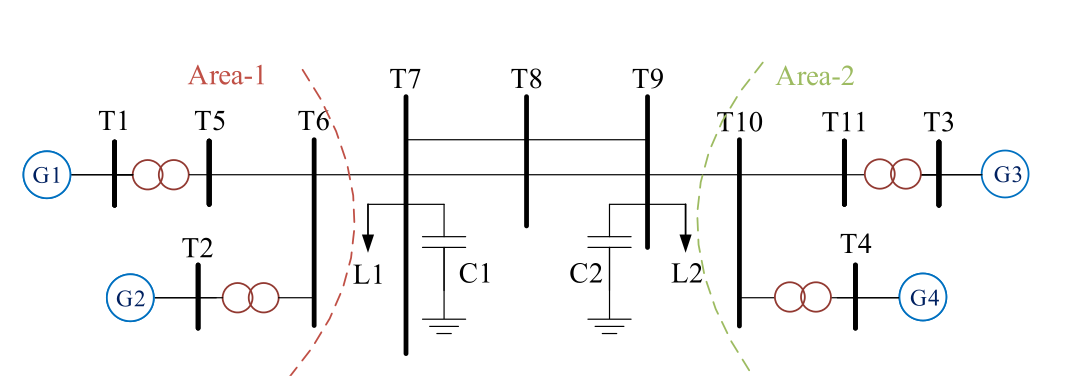
\includegraphics[width=0.92\textwidth]{images/system_figures/kundur_two_area_from_estimation2021.png}
    \caption{Μονογραμμικό διάγραμμα του \textenglish{\textit{Kundur Two-Area System}}~\cite{estimation2021}.}
    \label{fig:examined-kundur-system}
\end{figure}

Το πρότυπο σύστημα \textenglish{\textit{IEEE 39-Bus}} (\textenglish{\textit{New England Power System}}) αποτελεί ευρέως αποδεκτό σύστημα αναφοράς για μελέτες δυναμικής ευστάθειας και ταλαντώσεων ευρείας περιοχής. Αποτελείται από 39 ζυγούς, 10 γεννήτριες, εκ των οποίων η μία αναπαριστά ισοδύναμο διασύνδεσης μεγάλης έκτασης, 19 φορτία και 46 γραμμές μεταφοράς/μετασχηματιστές. Το σύστημα εμφανίζει τοπικούς και διασυνδετικούς ρυθμούς ταλάντωσης, καθιστώντας το κατάλληλο για την αξιολόγηση και σύγκριση της ακρίβειας των αλγορίθμων συσταδοποίησης υπό διαφορετικά σενάρια διείσδυσης ΑΠΕ και τύπων φορτίου~\cite{digsilent39,estimation2021,alzahrani2020dynamic}. Το μονογραμμικό του διάγραμμα και η διαίρεσή του σε τρεις περιοχές παρουσιάζονται στο Σχήμα~\ref{fig:examined-ieee39-system}.

Η κατάτμηση αυτή ομαδοποιεί τις γεννήτριες σύμφωνα με την ηλεκτρική τους θέση και τη συνεκτική δυναμική συμπεριφορά που αναμένεται να εμφανίζουν. Ειδικότερα, στην Περιοχή~1 εντάσσονται οι γεννήτριες $G_1$, $G_8$, $G_9$ και $G_{10}$, στην Περιοχή~2 οι $G_2$ και $G_3$, ενώ στην Περιοχή~3 οι $G_4$--$G_7$. Με τον διαχωρισμό αυτό, οι εκτιμώμενοι ρυθμοί μπορούν να εξετάζονται τόσο ανά περιοχή ελέγχου όσο και συνολικά για ολόκληρο το σύστημα.

Η διάκριση των περιοχών είναι ιδιαίτερα χρήσιμη για τη φυσική ερμηνεία των αποτελεσμάτων. Ταλαντώσεις μεταξύ γεννητριών της ίδιας περιοχής συνδέονται κυρίως με τοπικούς ρυθμούς, ενώ η συνεκτική κίνηση μιας ομάδας γεννητριών έναντι μιας άλλης χαρακτηρίζει διασυνδετικούς ρυθμούς. Συνεπώς, η χωρική πληροφορία του Σχήματος~\ref{fig:examined-ieee39-system} αξιοποιείται στη συνέχεια για την αξιολόγηση της ικανότητας των μεθόδων εκτίμησης και συσταδοποίησης να ανακτούν τις διαφορετικές μορφές ταλαντωτικής συμπεριφοράς.

\begin{figure}[htbp]
    \centering
    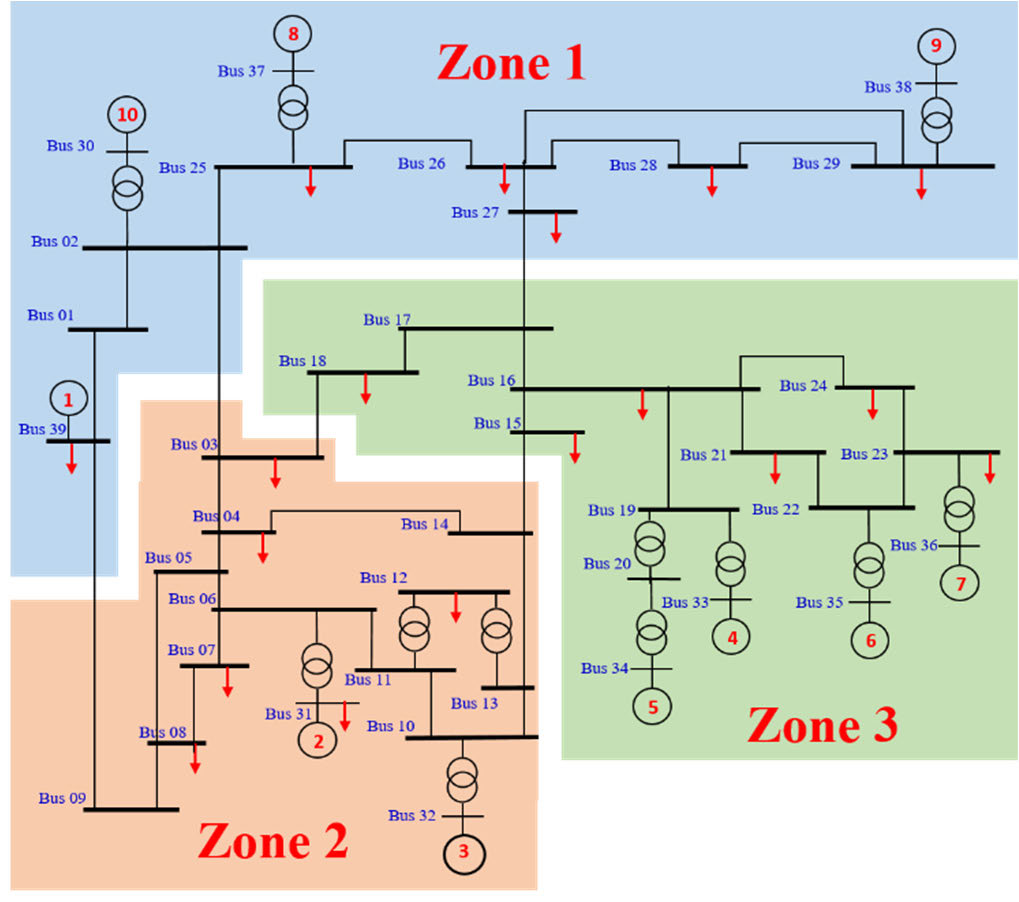
\includegraphics[width=0.82\textwidth]{images/system_figures/ieee39_three_zones_alzahrani2020.jpg}
    \caption{Μονογραμμικό διάγραμμα και διαίρεση του \textenglish{\textit{IEEE 39-Bus System}} σε τρεις περιοχές~\cite{alzahrani2020dynamic}.}
    \label{fig:examined-ieee39-system}
\end{figure}
\FloatBarrier


\kundursystemanalysistrue
\section{Ανάλυση του Συστήματος \textenglish{Kundur Two-Area}}
\subsection{Διαδικασία Παραγωγής Δεδομένων}
\ifkundursystemanalysis

Το πρώτο βήμα περιελάμβανε την εισαγωγή του συστήματος στο περιβάλλον του \textenglish{\textit{PowerFactory}} για τη δημιουργία των απαραίτητων χρονοσειρών. Συγκεκριμένα, εκτελέστηκε προσομοίωση \textenglish{RMS}, αφού πρώτα επιλύθηκε πρόβλημα ροής φορτίου για τον καθορισμό των αρχικών συνθηκών \textenglish{(Initial Conditions)}. Η συνολική διάρκεια της προσομοίωσης ορίστηκε στα $50$ s, με χρονικό βήμα ολοκλήρωσης (\textenglish{\textit{step size}}) $0.01$ s, επιτρέποντας την πλήρη καταγραφή της απόκρισης μετά την διαταραχή (\textenglish{\textit{ringdown}}) καθώς το σύστημα τείνει προς ένα νέο σημείο ισορροπίας. Για την παρακολούθηση των φαινομένων, εξήχθησαν οι μεταβλητές τάσης ($V$), ρεύματος ($I$), ενεργού ($P$) και άεργου ($Q$) ισχύος για καθεμία από τις γεννήτριες του συστήματος.

Ως συμβάν διαταραχής (\textenglish{\textit{event}}) για τη διέγερση των ηλεκτρομηχανικών ταλαντώσεων, ορίστηκε η προσωρινή αποσύνδεση της διασυνδετικής γραμμής \textenglish{07a\textendash{07b}}, η οποία συνδέει τις δύο περιοχές του συστήματος. Η γραμμή αποσυνδέθηκε τη χρονική στιγμή $t=0$~s και παρέμεινε εκτός λειτουργίας για $0.1$~s, πριν από την αυτόματη επανασύνδεσή της στο $t=0.1$~s. Η συγκεκριμένη διαταραχή ακολουθεί τη μεθοδολογία της βιβλιογραφίας για την παραγωγή αποκρίσεων \textenglish{\textit{ringdown}}, σύμφωνα με την οποία η προσωρινή αποσύνδεση μίας από τις δύο διασυνδετικές γραμμές του συστήματος και η επανασύνδεσή της μετά από $0.1$~s διεγείρει τους ρυθμούς ταλάντωσης του συστήματος~\cite{estimation2021}.

\subsubsection{Προεπεξεργασία Σημάτων.}
Πριν την εφαρμογή του αλγορίθμου MP, τα πρωτογενή δεδομένα του \textenglish{\textit{PowerFactory}} υποβλήθηκαν σε απαραίτητη ψηφιακή επεξεργασία (μέσω της γλώσσας Python), προκειμένου να εξασφαλιστεί η αξιοπιστία της ταυτοποίησης. Τα στάδια της προεπεξεργασίας περιελάμβαναν:

\begin{enumerate}
    \item \textbf{Αποκοπή Χρονοσειρών:} Μετά την εφαρμογή και την άρση της διαταραχής, η άμεση μεταβατική απόκριση μπορεί να επηρεάζεται από μη γραμμικότητες, υποβαθμίζοντας την ακρίβεια της ταυτοποίησης των ρυθμών ταλάντωσης~\cite{sfetkos2024measurement}. Για τον περιορισμό της επίδρασης της αρχικής μεταβατικής φάσης, απορρίφθηκαν τα δεδομένα έως $t=0.2$~s και η ανάλυση εφαρμόστηκε στο τμήμα της απόκρισης \textenglish{\textit{ringdown}} που διατηρήθηκε.
    \item \textbf{Αφαίρεση Γραμμικής Τάσης (\textenglish{\textit{Detrending}}):} Αφαιρέθηκε η βέλτιστη γραμμική τάση που περιλαμβάνει τη \textenglish{DC} συνιστώσα και τυχόν κλίση του σήματος.
    \item \textbf{Φιλτράρισμα:} Εφαρμόστηκε βαθυπερατό φίλτρο (\textenglish{\textit{Low-Pass}}) με συχνότητα αποκοπής $f_{c} = 10$ Hz για την απομάκρυνση υψίσυχνου θορύβου και συνιστωσών εκτός του πεδίου ενδιαφέροντος.
\end{enumerate}

\subsubsection{Στάδιο Ελέγχου και Φιλτραρίσματος των Δεδομένων.}
\label{subsec:data_screening}

Μετά την εξαγωγή των εκτιμώμενων ρυθμών από τις επιμέρους μεθόδους αναγνώρισης, εφαρμόστηκε στάδιο φιλτραρίσματος (\textenglish{\textit{data screening}}) των δεδομένων, με στόχο τη διασφάλιση της καταλληλότητάς τους για τη διαδικασία συσταδοποίησης. Το στάδιο αυτό δεν μετέβαλε τη διαδικασία υπολογισμού των ρυθμών, αλλά λειτούργησε ως βήμα προεπεξεργασίας πριν από την εφαρμογή των τεχνικών συσταδοποίησης. Η ανάγκη για φιλτράρισμα προέκυψε από το γεγονός ότι οι επιμέρους εκτιμήσεις που παράγονται από την ανάλυση MP ενδέχεται να περιλαμβάνουν τιμές που δεν σχετίζονται με πραγματικούς ηλεκτρομηχανικούς ρυθμούς ταλάντωσης, αλλά οφείλονται σε θόρυβο, αριθμητικές αβεβαιότητες ή μη φυσικούς ρυθμούς.

Σύμφωνα με τη σχετική βιβλιογραφία, οι \textenglish{\textit{inter-area}} ρυθμοί ταλάντωσης του \textenglish{\textit{Kundur Two-Area System}} εμφανίζονται στην περιοχή από $0.1$~Hz έως $0.7$~Hz, ενώ οι \textenglish{\textit{intra-area}} ρυθμοί ταλάντωσης εντοπίζονται στην περιοχή από $0.7$~Hz έως $2.0$~Hz~\cite{estimation2021}. Συνεπώς, διατηρήθηκαν μόνο οι εκτιμήσεις με συχνότητα εντός του διαστήματος $[0.1,\,2.0]$~Hz και με αρνητικό ρυθμό απόσβεσης που να ικανοποιεί το όριο $\sigma \leq -10^{-3}$. Έτσι προέκυψε ένα καθαρό σύνολο δεδομένων, κατάλληλο για την εφαρμογή των τεχνικών συσταδοποίησης που αξιοποιήθηκαν στη συνέχεια της ανάλυσης.

\else
Παρόμοια με την περίπτωση του \textenglish{\textit{Kundur Two-Area System}}, εκτελέστηκε προσομοίωση \textenglish{RMS} διάρκειας $50$ s με χρονικό βήμα $0.01$ s και εξήχθησαν οι μεταβλητές $V$, $I$, $P$ και $Q$ για κάθε γεννήτρια. Ως διαταραχή εφαρμόστηκε αύξηση της ενεργού ισχύος $P$ του φορτίου $3$ (\textenglish{\textit{Load 03}}) κατά $2\%$ τη χρονική στιγμή $t=0$ s~\cite{digsilent39,sfetkos2024measurement}.

Στα παραγόμενα σήματα εφαρμόστηκαν τα ίδια στάδια προεπεξεργασίας και φιλτραρίσματος με την περίπτωση του συστήματος Kundur. Οι ρυθμοί αναφοράς του \textenglish{\textit{IEEE 39-Bus System}} βρίσκονται επίσης εντός της περιοχής $[0.1,\,2.0]$~Hz~\cite{sarkar2024drga} και, επομένως, χρησιμοποιήθηκαν τα ίδια κριτήρια διατήρησης των εκτιμήσεων.
\fi

\subsection{Εφαρμογή της Μεθόδου Matrix Pencil}
\ifkundursystemanalysis
Η ανάλυση των αποκρίσεων διαταραχών μέσω τεχνικών ταυτοποίησης συστήματος αποτελεί μια μέθοδο για την παρακολούθηση της δυναμικής ευστάθειας \cite{modal2018}. Η διαδικασία της ταυτοποίησης βασίστηκε στην ανάλυση των προεπεξεργασμένων σημάτων $V$, $I$, $P$ και $Q$ μέσω του αλγορίθμου MP. Σύμφωνα με τις απαιτήσεις της διερεύνησης, η μέθοδος εφαρμόστηκε με δύο διαφορετικές προσεγγίσεις για τον καθορισμό της τάξης $n$ του συστήματος.

\begin{enumerate}
    \item \textbf{Καθορισμένη Τάξη:} Χρησιμοποιήθηκαν σταθερές τιμές τάξης $n \in \{2, 4, 6\}$.
    \item \textbf{Αυτόματος Καθορισμός Τάξης:} Για τον αυτόματο καθορισμό της τάξης του μοντέλου εφαρμόστηκε ο αλγόριθμος της~\cite{estimation2021}. Εξετάστηκαν τρία διαφορετικά επίπεδα ανοχής, $\tau \in \{1, 0.1, 0.01\}$. Ο αλγόριθμος επιλέγει αυτόματα την τάξη του μοντέλου μέσω μιας διαδικασίας διαδοχικής βελτίωσης της ανακατασκευής του σήματος. Στο πλαίσιο αυτό, η τάξη αυξανόταν μέχρι η μεταβολή του συντελεστή $R^2$ μεταξύ δύο διαδοχικών ανακατασκευών να γίνει μικρότερη απο $\tau$.
\end{enumerate}
\else
Παρόμοια με την περίπτωση του συστήματος Kundur, η μέθοδος MP εφαρμόστηκε στα προεπεξεργασμένα σήματα $V$, $I$, $P$ και $Q$, τόσο με καθορισμένη όσο και με αυτόματα επιλεγόμενη τάξη. Η μόνη διαφοροποίηση ήταν ότι, εκτός από τις σταθερές τιμές $n\in\{2,4,6\}$, εξετάστηκε επιπλέον η τιμή $n=8$, λόγω του μεγαλύτερου πλήθους ηλεκτρομηχανικών ρυθμών του \textenglish{\textit{IEEE 39-Bus System}}~\cite{sarkar2024drga}. Για τον αυτόματο καθορισμό της τάξης χρησιμοποιήθηκαν τα ίδια επίπεδα ανοχής $\tau\in\{1,0.1,0.01\}$.
\fi

\subsection{Μαθηματική Ανακατασκευή και Πιστότητα}
\ifkundursystemanalysis
Για κάθε σενάριο ταυτοποίησης εξήχθησαν οι παράμετροι των αναγνωρισμένων ρυθμών ταλάντωσης: το πλάτος ($A_{i}$), ο ρυθμός απόσβεσης ($\sigma_{i}$), η συχνότητα ($f_{i}$ σε Hz) και η φάση ($\varphi_{i}$). Η μαθηματική ανακατασκευή του σήματος $\hat{y}(t)$ πραγματοποιήθηκε μέσω της σχέσης:

\begin{equation}
\hat{y}(t)=\sum_{i=1}^{n}A_{i}e^{\sigma_{i}t}\cos(2\pi f_{i}t+\varphi_{i})
\label{eq:reconstruction}
\end{equation}

Η πιστότητα της ανακατασκευής αξιολογήθηκε μέσω του συντελεστή προσδιορισμού $R^{2}$ και της τετραγωνικής ρίζας του μέσου τετραγωνικού σφάλματος (RMSE), οι οποίοι υπολογίζονται αντίστοιχα από τις σχέσεις:

\begin{equation}
R^2=1-\frac{\displaystyle\sum_{k=1}^{N}\left(y_k-\hat{y}_k\right)^2}
{\displaystyle\sum_{k=1}^{N}\left(y_k-\bar{y}\right)^2}
\label{eq:reconstruction_r2}
\end{equation}

\begin{equation}
\mathrm{RMSE}=\sqrt{\frac{1}{N}\sum_{k=1}^{N}\left(y_k-\hat{y}_k\right)^2}
\label{eq:reconstruction_rmse}
\end{equation}

όπου $y_k$ και $\hat{y}_k$ είναι αντίστοιχα η πραγματική και η ανακατασκευασμένη τιμή του σήματος στο $k$-οστό δείγμα, $\bar{y}$ είναι η μέση τιμή του πραγματικού σήματος και $N$ το συνολικό πλήθος των δειγμάτων. Τιμές του $R^2$ κοντά στη μονάδα και μικρές τιμές του RMSE υποδηλώνουν υψηλή πιστότητα ανακατασκευής. Η διαδικασία αυτή εξασφαλίζει ότι οι ταυτοποιημένοι ρυθμοί ταλάντωσης αντιπροσωπεύουν με ακρίβεια τη φυσική απόκριση των εξεταζόμενων συστημάτων και δεν αποτελούν μαθηματικά σφάλματα της προσέγγισης.
\else
Η ανακατασκευή των σημάτων και η αξιολόγηση της πιστότητάς της πραγματοποιήθηκαν παρόμοια με την περίπτωση του συστήματος Kundur, μέσω των~(\ref{eq:reconstruction})-(\ref{eq:reconstruction_rmse}).
\fi



\subsection{Αποτελέσματα και Γραφικές Παραστάσεις}

\subsubsection{Απεικόνιση Ρυθμού Απόσβεσης και Συχνότητας}
\ifkundursystemanalysis
\label{sec:modal_and_reconstruction_plots}
\fi
Ως αποτέλεσμα της εφαρμογής του αλγορίθμου MP, ελήφθησαν τα διαγράμματα της παρούσας παραγράφου, στα οποία παρουσιάζεται η κατανομή των ιδιοτιμών στο μιγαδικό επίπεδο για τα μετρούμενα μεγέθη των γεννητριών των συστημάτων. Συγκεκριμένα, στον οριζόντιο άξονα παρουσιάζεται ο ρυθμός απόσβεσης, ο οποίος αποτελεί το πραγματικό μέρος των ιδιοτιμών, ενώ στον κατακόρυφο άξονα η συχνότητα ταλάντωσης σε Hz.


\ifkundursystemanalysis
\begin{figure}[H]
    \centering
    \includegraphics[width=0.94\textwidth,height=0.82\textheight,keepaspectratio]{\preliminaryfigurepath plots/modal_maps/pdf/All_Generators_Grid.pdf}
    \caption{Κατανομή ιδιοτιμών (\textit{Πραγματικό Μέρος έναντι Συχνότητας}) για τις γεννήτριες $G_1$-$G_4$ του \textenglish{\textit{Kundur Two-Area System}}.}
    \label{fig:poles_distribution_all_kundur}
\end{figure}
\else
\begin{figure}[!htbp]
    \centering
    \includegraphics[width=0.94\textwidth,height=0.82\textheight,keepaspectratio]{\ieeeThirtyNinePathanalysis/Load03_Pplus2_50s_0.2_to_end_reset/plots/modal_maps/pdf/All_Generators_Grid.pdf}
    \caption{Κατανομή ιδιοτιμών (\textit{Πραγματικό Μέρος έναντι Συχνότητας}) για τις γεννήτριες $G_1$-$G_{10}$ του \textenglish{\textit{IEEE 39-Bus System}}.}
    \label{fig:poles_distribution_all_ieee39}
\end{figure}
\fi


\ifkundursystemanalysis
Στο Σχήμα~\ref{fig:poles_distribution_all_kundur} αποτυπώνεται η κατανομή των ταυτοποιημένων ιδιοτιμών για τις τέσσερις γεννήτριες του \textenglish{\textit{Kundur Two-Area System}} ($G_1$-$G_4$).
\else
Στο Σχήμα~\ref{fig:poles_distribution_all_ieee39} παρουσιάζεται η κατανομή των ιδιοτιμών για τις δέκα γεννήτριες του \textenglish{\textit{IEEE 39-Bus System}}.
\fi
Το σύνολο των ηλεκτρομηχανικών ιδιοτιμών εντοπίζεται στο αριστερό ημιεπίπεδο ($\sigma$ < 0), υποδεικνύοντας τη θετική απόσβεση των ταλαντώσεων.
Ακόμα, καταγράφονται στον οριζόντιο άξονα και ιδιοτιμές με μηδενική συχνότητα, οι οποίες δεν αντιστοιχούν σε κύριους ρυθμούς ταλάντωσης, αλλά σε ρυθμούς που σχετίζονται με τα συστήματα ελέγχου, καθώς και σε ψευδείς ρυθμούς \textenglish{(spurious modes)}.

\subsubsection{Αξιολόγηση Πιστότητας Ανακατασκευής}
Για την επαλήθευση της εγκυρότητας των ταυτοποιημένων ρυθμών που εξήχθησαν στην προηγούμενη ενότητα, πραγματοποιήθηκε μαθηματική ανακατασκευή των σημάτων στο πεδίο του χρόνου. Εξετάστηκαν οι επιμέρους προσεγγίσεις σταθερής τάξης $n$ και ανοχής $\tau$ και, για κάθε σήμα, επιλέχθηκε η μέθοδος που απέδωσε τη μεγαλύτερη τιμή του συντελεστή προσδιορισμού $R^2$. Στο
\ifkundursystemanalysis
Σχήμα~\ref{fig:best_recon_g1_kundur}
\else
Σχήμα~\ref{fig:best_recon_g9_ieee39}
\fi
παρουσιάζεται ένα αντιπροσωπευτικό παράδειγμα, στο οποίο συγκρίνονται τα αρχικά φιλτραρισμένα σήματα με τις αντίστοιχες ανακατασκευασμένες κυματομορφές που προέκυψαν από τη μέθοδο MP.

\ifkundursystemanalysis
\begin{figure}[H]
    \centering
    \captionsetup{font=small,skip=4pt}
    \includegraphics[width=0.96\textwidth,height=0.72\textheight,keepaspectratio]{\preliminaryfigurepath stats/pdf/10_best_reconstruction_g1_2x2.pdf}
    \caption{Βέλτιστη μαθηματική ανακατασκευή των σημάτων ($V, I, P, Q$) για τη γεννήτρια $G_1$ του \textenglish{\textit{Kundur Two-Area System}} με βάση τον μέγιστο συντελεστή προσδιορισμού $R^2$.}
    \label{fig:best_recon_g1_kundur}
\end{figure}
\else
\begin{figure}[H]
    \centering
    \captionsetup{font=small,skip=4pt}
    \includegraphics[width=0.96\textwidth,height=0.72\textheight,keepaspectratio]{\ieeeThirtyNinePathanalysis/Load03_Pplus2_50s_0.2_to_end_reset/stats/pdf/10_best_reconstruction_g9_2x2.pdf}
    \caption{Βέλτιστη μαθηματική ανακατασκευή των σημάτων ($V, I, P, Q$) για τη γεννήτρια $G_{9}$ του \textenglish{\textit{IEEE 39-Bus System}} με βάση τον μέγιστο συντελεστή προσδιορισμού $R^2$.}
    \label{fig:best_recon_g9_ieee39}
\end{figure}
\fi

Όπως παρατηρείται στο αντιπροσωπευτικό παράδειγμα, επιτυγχάνεται εξαιρετική σύμπτωση μεταξύ των αρχικών και των ανακατασκευασμένων κυματομορφών. Αξίζει να σημειωθεί, ωστόσο, ότι η βέλτιστη ανακατασκευή δεν προκύπτει από μία καθολική επιλογή τάξης ή ανοχής, γεγονός που επιβεβαιώνει την αναγκαιότητα εξέτασης πολλαπλών προσεγγίσεων.

Τέλος, η ταύτιση των κυματομορφών αναλύεται στο χρονικό παράθυρο της γραμμικής συμπεριφοράς, δηλαδή για t > 0.2 s. Η υψηλή πιστότητα της ανακατασκευής επιβεβαιώνει την ορθή επιλογή του παραθύρου ανάλυσης, καθώς και την αποτελεσματικότητα της προεπεξεργασίας των σημάτων.

\FloatBarrier
\subsubsection{Ταυτοποίηση Κυρίαρχων Ρυθμών Ταλάντωσης}
\ifkundursystemanalysis
\label{subsec:overall_evaluation}

Η συνολική αξιολόγηση της δυναμικής του συστήματος πραγματοποιήθηκε με βάση τα διαγράμματα της Ενότητας \ref{sec:modal_and_reconstruction_plots} και το Διάγραμμα Φυσαλίδων (\textenglish{\textit{Bubble Map}}) του Σχήματος~\ref{fig:bubble_map_kundur}. Με τον τρόπο αυτό αποτυπώθηκαν συνολικά η συχνότητα, η απόσβεση και η ενέργεια των ταυτοποιημένων ρυθμών ταλάντωσης.
Για την αποτύπωση της σχετικής σημασίας κάθε ρυθμού ταλάντωσης στα Διαγράμματα Φυσαλίδων , υπολογίστηκε η ενέργεια κάθε ρυθμού ταλάντωσης σύμφωνα με:
\begin{equation}
\omega_i = 2\pi f_i
\end{equation}
\begin{equation}
\label{eq:pole_energy}
E_i = \frac{1}{2}\omega_i^2 \alpha_i^2
\end{equation}
όπου $f_i$ είναι η συχνότητα και $\alpha_i$ το πλάτος του $i$-οστού ρυθμού. Το μέγεθος κάθε φυσαλίδας είναι ανάλογο της ποσότητας $E_i$ \cite{sfetkos2024measurement}.

Η συγκεκριμένη απεικόνιση παρέχει τη συνολικότερη εικόνα της ταυτοποίησης και επιβεβαιώνει τα ευρήματα που παρουσιάστηκαν στην Ενότητα \ref{sec:modal_and_reconstruction_plots}. Παρατηρείται συγκέντρωση εκτιμήσεων σε τρεις βασικές περιοχές συχνοτήτων: πολύ κοντά στο $0$ Hz, στην περιοχή $0.5-0.6$ Hz και γύρω από το $1.1$ Hz. Η πρώτη περιοχή συνδέεται κυρίως με αργές μη ταλαντωτικές συνιστώσες και με ψευδείς ρυθμούς της μεθόδου, ενώ οι υπόλοιπες αντιστοιχούν σε κυρίαρχους ρυθμούς ταλάντωσης του συστήματος.
% Παράλληλα, η κατανομή των ιδιοτιμών ως προς τον ρυθμό απόσβεσης $\sigma$ δείχνει ότι οι ταλαντώσεις εμφανίζουν γενικά θετική απόσβεση, καθώς τα περισσότερα σημεία εντοπίζονται στο αριστερό ημιεπίπεδο.

Για το σύστημα \textenglish{\textit{Kundur Two-Area}}, η ποσοτική αποτύπωση των κυρίαρχων ρυθμών ταλάντωσης παρουσιάζεται στον Πίνακα~\ref{tab:summary_modes}. Οι τιμές του πίνακα επιλέχθηκαν με βάση τη μέγιστη ενέργεια στις περιοχές συχνοτήτων $0.4-0.6$~Hz και $1.0-1.1$~Hz, σύμφωνα με την~(\ref{eq:pole_energy}). Στο Σχήμα~\ref{fig:bubble_map_kundur}, οι μεγαλύτερες φυσαλίδες στην περιοχή των $0.54$~Hz εμφανίζονται κυρίως στα σήματα ενεργού ισχύος των γεννητριών $G_3$ και $G_4$, αναδεικνύοντας την υψηλή ενεργειακή συμμετοχή του κυρίαρχου διασυνδετικού ρυθμού.


\raggedbottom
\begin{figure}[H]
    \centering
    \includegraphics[width=0.98\textwidth,keepaspectratio,trim=15pt 65pt 10pt 35pt,clip]{\preliminaryfigurepath stats/pdf/5_bubble_map.pdf}
    \caption{Διαγράμματα Φυσαλίδων-Συγκεντρωτική απεικόνιση συχνότητας, απόσβεσης και ενέργειας των ταυτοποιημένων ρυθμών ταλάντωσης.}
    \label{fig:bubble_map_kundur}
\end{figure}

Σημαντική ενέργεια παρουσιάζουν επίσης οι εκτιμήσεις στην περιοχή $1.0-1.1$~Hz, ιδιαίτερα στα σήματα ενεργού ισχύος, οι οποίες αντιστοιχούν στους τοπικούς ρυθμούς του συστήματος. Αντίθετα, οι συνιστώσες πολύ κοντά στα $0$~Hz εμφανίζουν γενικά μικρότερες φυσαλίδες και, συνεπώς, χαμηλότερη ενέργεια, γεγονός που υποστηρίζει τον διαχωρισμό τους από τους κυρίαρχους ηλεκτρομηχανικούς ρυθμούς. Οι τοπικοί ρυθμοί εμφανίζονται επιπλέον με μεγαλύτερες απόλυτες τιμές απόσβεσης σε σχέση με τον διασυνδετικό ρυθμό.

\else
Η συνολική αξιολόγηση πραγματοποιήθηκε παρόμοια με την περίπτωση του συστήματος Kundur, με βάση την κατανομή των εκτιμώμενων ρυθμών και το Διάγραμμα Φυσαλίδων του Σχήματος~\ref{fig:bubble_map_ieee39}. Η ενέργεια των ταυτοποιημένων ρυθμών υπολογίστηκε σύμφωνα με την~(\ref{eq:pole_energy}).

\begin{figure}[!htbp]
    \centering
    \includegraphics[width=0.94\textwidth,height=0.64\textheight,keepaspectratio,trim=20pt 260pt 15pt 100pt,clip]{\ieeeThirtyNinePathanalysis/Load03_Pplus2_50s_0.2_to_end_reset/stats/pdf/5_bubble_map_single_panel.pdf}
    \caption{Διαγράμματα Φυσαλίδων-Συγκεντρωτική απεικόνιση συχνότητας, απόσβεσης και ενέργειας των ταυτοποιημένων ρυθμών ταλάντωσης.}
    \label{fig:bubble_map_ieee39}
\end{figure}


Αξίζει να σημειωθεί ότι στο \textenglish{\textit{IEEE 39-Bus System}} η αντίστοιχη ποσοτική ερμηνεία δεν είναι εξίσου άμεση, λόγω της μεγαλύτερης πολυπλοκότητας του συστήματος. Για τον λόγο αυτό, η αξιολόγηση του \textenglish{\textit{IEEE 39-Bus System}} βασίζεται κυρίως στις συνολικές γραφικές απεικονίσεις και στη συγκριτική ερμηνεία των αποτελεσμάτων.
\fi

\ifkundursystemanalysis
\begin{table}[h]
\centering
\caption{Σύνοψη Κυρίαρχων Ρυθμών Ταλάντωσης με Κριτήριο τη Μέγιστη Ενέργεια}
\label{tab:summary_modes}
\resizebox{\textwidth}{!}{%
\begin{tabular}{cccc | ccc}
\toprule
\multicolumn{4}{c}{\textbf{Inter-area ρυθμός ταλάντωσης ($0.4-0.6$ Hz)}} & \multicolumn{3}{c}{\textbf{Intra-area ρυθμοί ταλάντωσης ($1.0-1.1$ Hz)}} \\
\cmidrule(lr){1-4}\cmidrule(lr){5-7}
\textbf{Γεν.} & \textbf{σήμα} & \textbf{$f$ [Hz]} & \textbf{$\sigma$ [rad/s]} & \textbf{σήμα} & \textbf{$f$ [Hz]} & \textbf{$\sigma$ [rad/s]} \\
\midrule
    G1 & P & 0.543 & -0.125 & P & 1.043 & -0.838 \\
    & Q & 0.543 & -0.126 & Q & 1.038 & -0.766 \\
    & V & 0.542 & -0.131 & V & $-$ & $-$ \\
    & I & 0.543 & -0.125 & I & 1.040 & -0.799 \\
    \midrule
    G2 & P & 0.539 & -0.144 & P & 1.059 & -0.773 \\
    & Q & 0.543 & -0.127 & Q & 1.079 & -0.664 \\
    & V & 0.543 & -0.129 & V & $-$ & $-$ \\
    & I & 0.543 & -0.126 & I & 1.052 & -0.776 \\
    \midrule
    G3 & P & 0.544 & -0.136 & P & 1.087 & -0.697 \\
    & Q & 0.543 & -0.124 & Q & 1.025 & -0.848 \\
    & V & 0.543 & -0.130 & V & 1.017 & -1.066 \\
    & I & 0.544 & -0.137 & I & 1.088 & -0.727 \\
    \midrule
    G4 & P & 0.543 & -0.127 & P & 1.091 & -0.849 \\
    & Q & 0.543 & -0.131 & Q & $-$ & $-$ \\
    & V & 0.543 & -0.130 & V & 1.027 & -0.796 \\
    & I & 0.543 & -0.127 & I & 1.094 & -0.817 \\
\bottomrule
\end{tabular}
}
\end{table}
\fi

\subsubsection{Αξιολόγηση των Εκτιμήσεων μέσω του Δείκτη \textit{MAD}}
\ifkundursystemanalysis
\label{subsec:mad_evaluation}

Μετά το στάδιο ελέγχου και φιλτραρίσματος των δεδομένων, πραγματοποιήθηκε ποσοτική
αξιολόγηση των εκτιμώμενων ρυθμών ταλάντωσης που προέκυψαν από τη μέθοδο \textenglish{\textit{MP}} ως προς
τους θεωρητικούς ρυθμούς ταλάντωσης των εξεταζόμενων συστημάτων. Για τον σκοπό αυτό χρησιμοποιήθηκε
ο δείκτης \textenglish{\textit{MAD}}~\cite{modal2018}.

\begin{equation}
\mathrm{MAD}_i = \mathrm{median}\left(\left| \hat{\lambda}_{i,j} - \lambda_i \right|\right)
\label{eq:mad_definition}
\end{equation}
όπου \(\hat{\lambda}_{i,j}\) είναι η \(j\)-οστή εκτίμηση της ιδιοτιμής του \(i\)-οστού
ρυθμού ταλάντωσης και \(\lambda_i\) η αντίστοιχη θεωρητική ιδιοτιμή αναφοράς.

Ως ρυθμοί αναφοράς λήφθηκαν οι τρεις κυρίαρχοι ρυθμοί ταλάντωσης του
συστήματος Kundur~\cite{estimation2021}, οι οποίοι παρουσιάζονται στον
Πίνακα~\ref{tab:kundur_reference_modes}. Ο πρώτος ρυθμός ταλάντωσης αντιστοιχούσε στον \textenglish{\textit{inter-area}}
ρυθμό ταλάντωσης του συστήματος, ενώ οι δύο επόμενοι στους \textenglish{\textit{intra-area}} ρυθμούς ταλάντωσης των δύο περιοχών.


\begin{table}[!htbp]
\centering
\caption{Ρυθμοί αναφοράς του συστήματος Kundur Two-Area System.}
\label{tab:kundur_reference_modes}
\begin{tabular}{ccc}
\toprule
\textbf{ρυθμός ταλάντωσης} & \textbf{$f$ [Hz]} & \textbf{$\sigma$ [rad/s]} \\
\midrule
\textenglish{\textit{Inter-area}}   & 0.540 & -0.127 \\
\textenglish{\textit{Intra-area}} 1 & 1.083 & -0.603 \\
\textenglish{\textit{Intra-area}} 2 & 1.119 & -0.631 \\
\bottomrule
\end{tabular}
\end{table}
\else
Η αξιολόγηση πραγματοποιήθηκε παρόμοια με την περίπτωση του συστήματος Kundur, μέσω του δείκτη \textenglish{\textit{MAD}} της~(\ref{eq:mad_definition}). Ως ρυθμοί αναφοράς λήφθηκαν οι εννέα κυρίαρχοι ρυθμοί που παρουσιάζονται στον Πίνακα~\ref{tab:ieee39_reference_modes}~\cite{sarkar2024drga}.

\begin{table}[!htbp]
\centering
\caption{Ρυθμοί αναφοράς του συστήματος IEEE 39-Bus.}
\label{tab:ieee39_reference_modes}
\resizebox{\textwidth}{!}{%
\begin{tabular}{cccccc}
\toprule
\textbf{ρυθμός ταλάντωσης} & \textbf{$f$ [Hz]} & \textbf{$\sigma$ [rad/s]}  & \textbf{γεννήτριες} & \textbf{περιοχές} & \textbf{τύπος} \\
\midrule
ρυθμός ταλάντωσης 1 & 0.6062 & -0.0800  & 1$-$9 vs. 10 & 1-3 &  Inter-area\\
ρυθμός ταλάντωσης 2 & 0.9497 & -0.1065  & 1, 8, 9 vs. 4, 5, 6, 7 & 1, 2 & Inter-area \\
ρυθμός ταλάντωσης 3 & 1.0312 & -0.2558  & 2, 3 vs. 4, 5 & 2, 3 & Inter-area\\
ρυθμός ταλάντωσης 4 & 1.1211 & -0.3373  & 2, 3 vs. 6, 7 &  2, 3 & Inter-area \\
ρυθμός ταλάντωσης 5 & 1.3155 & -0.4033  & 2 vs. 3 &  2 & Intra-area\\
ρυθμός ταλάντωσης 6 & 1.2851 & -0.3458  & 1 vs. 8, 9 & 1 & Intra-area\\
ρυθμός ταλάντωσης 7 & 1.4953 & -0.7033  & 4 vs. 5 & 3 & Intra-area\\
ρυθμός ταλάντωσης 8 & 1.5202 & -0.6010  & 5, 7 vs. 4, 6 & 3 & Intra-area\\
ρυθμός ταλάντωσης 9 & 1.5468 & -0.6376  & 1 vs. 8 & 1 & Intra-area\\
\bottomrule
\end{tabular}
}
\end{table}
\fi

\ifkundursystemanalysis
Για τον υπολογισμό του MAD χρησιμοποιήθηκαν οι εκτιμήσεις που παρέμειναν μετά το
στάδιο ελέγχου δεδομένων της Παραγράφου~\ref{subsec:data_screening}. Για κάθε μέθοδο συσταδοποίησης, κάθε τελική συστάδα αντιστοιχίζεται στο πλησιέστερο ρυθμό αναφοράς μέσω του
αντιπροσώπου της (κέντρο ή medoid) στο επίπεδο $(\sigma,\omega)$. Ο MAD κάθε ρυθμού ταλάντωσης είναι η διάμεσος των αποστάσεων
των εκτιμήσεων που ανήκουν στις συστάδες οι οποίες αντιστοιχίστηκαν σε αυτό. Με τον τρόπο
αυτό, ο δείκτης MAD παρείχε ένα συνοπτικό και ανθεκτικό μέτρο της απόκλισης των τελικών
εκτιμήσεων από τις θεωρητικές θέσεις των κυρίαρχων ρυθμών ταλάντωσης του συστήματος και τα βασικά αποτελέσματα των υπολογισμών συνοψίζονται στον Πίνακα~\ref{tab:mad_summary_kundur} τα οποία σχολιάζονται στην Ενότητα~\ref{sec:kundur-clustering-results}.




\begin{table}[!t]
\centering
\caption{MAD ανά μέθοδο συσταδοποίησης για το Kundur Two-Area System.}
\label{tab:mad_summary_kundur}
\begin{tabular}{ccccc}
\toprule
\textbf{ρυθμός ταλάντωσης} & \multicolumn{2}{c}{\textbf{k-Means}} & \multicolumn{2}{c}{\textbf{k-Medoids}} \\
\cmidrule(lr){2-3}\cmidrule(l){4-5}
 & \textbf{πλήθος} & \textbf{MAD} & \textbf{πλήθος} & \textbf{MAD} \\
\midrule
\textenglish{\textit{Inter-area}}   & 98 & 0.0190 & 98 & 0.0190 \\
\textenglish{\textit{Intra-area}} 1 & 45 & 0.2584 & 45 & 0.2584 \\
\textenglish{\textit{Intra-area}} 2 & 0  & $-$     & 0  & $-$     \\
\bottomrule
\end{tabular}
\end{table}
\else
Για το \textenglish{\textit{IEEE 39-Bus System}}, τα αποτελέσματα του δείκτη MAD παρουσιάζονται στον
Πίνακα~\ref{tab:mad_summary_ieee39} ανά ρυθμό αναφοράς. Για ρυθμούς ταλάντωσης χωρίς καμία
αντιστοιχισμένη εκτίμηση καταγράφεται πλήθος ίσο με μηδέν. Παρατηρείται ότι η καλύτερη
συμφωνία εμφανίζεται κυρίως για τους ρυθμούς ταλάντωσης~3 και~4, οι οποίοι παρουσιάζουν τις μικρότερες τιμές MAD. Αντίθετα, ο ρυθμός ταλάντωσης~1 συγκεντρώνει το μεγαλύτερο πλήθος εκτιμήσεων ($265$), όπως ήταν αναμενόμενο καθώς είναι παρατηρίσιμο από όλες τις περιοχές ελέγχου του συστήματος, αλλά και σαφώς μεγαλύτερη τιμή δείκτη \textenglish{\textit{MAD}} ($0.3437$). Σημειώνεται ότι, για το \textenglish{\textit{IEEE 39-Bus System}}, οι εκτιμήσεις κάθε περιοχής ελέγχου αντιστοιχίζονται μόνο στους ρυθμούς αναφοράς για τους οποίους η βιβλιογραφία υποδεικνύει συμμετοχή των αντίστοιχων γεννητριών~\cite{sarkar2024drga}. Με τον τρόπο αυτό, οι αντιστοιχίσεις των εκτιμήσεων στους ρυθμούς αναφοράς παραμένουν συμβατές με τη φυσική ερμηνεία των ρυθμών ταλάντωσης του συστήματος.
Συνολικά, τα αποτελέσματα για το \textenglish{\textit{IEEE 39-Bus System}} εμφανίζουν μεγαλύτερη διασπορά σε σύγκριση με εκείνα του \textenglish{\textit{Kundur Two-Area System}}, γεγονός που είναι αναμενόμενο λόγω της σημαντικά μεγαλύτερης πολυπλοκότητας του συστήματος.

\begin{table}[!t]
\centering
\caption{MAD ανά μέθοδο συσταδοποίησης για το IEEE 39-Bus.}
\label{tab:mad_summary_ieee39}
\begin{tabular}{cccccc}
\toprule
\textbf{ρυθμός ταλάντωσης} & \textbf{$f$ [Hz]} & \multicolumn{2}{c}{\textbf{k-Means}} & \multicolumn{2}{c}{\textbf{k-Medoids}} \\
\cmidrule(lr){3-4}\cmidrule(l){5-6}
 & & \textbf{πλήθος} & \textbf{MAD} & \textbf{πλήθος} & \textbf{MAD} \\
\midrule
ρυθμός ταλάντωσης 1 & 0.6062 & 265 & 0.3437 & 265 & 0.3437 \\
ρυθμός ταλάντωσης 2 & 0.9497 & 34  & 1.0485 & 0   & $-$     \\
ρυθμός ταλάντωσης 3 & 1.0312 & 19  & 0.2780 & 19  & 0.2780 \\
ρυθμός ταλάντωσης 4 & 1.1211 & 37  & 0.2883 & 41  & 0.2945 \\
ρυθμός ταλάντωσης 5 & 1.3155 & 0   & $-$     & 0   & $-$     \\
ρυθμός ταλάντωσης 6 & 1.2851 & 3   & 0.9201 & 37  & 1.0708 \\
ρυθμός ταλάντωσης 7 & 1.4953 & 4   & 0.6989 & 0   & $-$     \\
ρυθμός ταλάντωσης 8 & 1.5202 & 0   & $-$     & 0   & $-$     \\
ρυθμός ταλάντωσης 9 & 1.5468 & 0   & $-$     & 0   & $-$     \\
\bottomrule
\end{tabular}
\end{table}
\fi

Στη συνέχεια, η ανάλυση συμπληρώθηκε με εφαρμογή τεχνικών συσταδοποίησης στις
εκτιμήσεις ρυθμών ταλάντωσης, με στόχο τη διερεύνηση της εσωτερικής τους οργάνωσης στο επίπεδο
συχνότητας$-$απόσβεσης και την ανάδειξη των κυρίαρχων περιοχών συγκέντρωσης.


\subsubsection{Αποτελέσματα Συσταδοποίησης}
\ifkundursystemanalysis
\label{sec:kundur-clustering-results}
Στόχος της συσταδοποίησης ήταν η ομαδοποίηση των ταυτοποιημένων ρυθμών ταλάντωσης, με σκοπό τον εντοπισμό των κυρίαρχων ρυθμών ταλάντωσης του συστήματος και τη διερεύνηση του κατά πόσο οι διαφορετικές μέθοδοι συσταδοποίησης συγκλίνουν σε κοινές περιοχές συχνοτήτων και αποσβέσεων. Όπως περιγράφηκε προηγουμένως στην παράγραφο \ref{subsec:data_screening}, εφαρμόστηκε φιλτράρισμα των εκτιμήσεων, διατηρώντας μόνο εκείνες με συχνότητες εντός του διαστήματος $[0.1,\,2.0]$~Hz, προκειμένου να διασφαλιστεί ότι οι συστάδες που προκύπτουν αντιστοιχούν σε φυσικούς ρυθμούς ταλάντωσης του συστήματος.

Για τη διερεύνηση της δομής των δεδομένων εφαρμόστηκαν οι αλγόριθμοι συσταδοποίησης \textenglish{\textit{k-Means}} και \textenglish{\textit{k-Medoids}}~\cite{macqueen1967some},~\cite{kaufman2009finding} για τιμές \(k = 1,2,\ldots,10\). Η επιλογή του βέλτιστου αριθμού συστάδων βασίστηκε σε δύο συμπληρωματικά κριτήρια: τη μέθοδο \textenglish{\textit{Elbow}}, για τον εντοπισμό του σημείου καμπής της καμπύλης κόστους, και τη μέθοδο \textenglish{\textit{Silhouette}}~\cite{ROUSSEEUW198753}, για την αξιολόγηση της συνοχής και του διαχωρισμού των συστάδων. Για τον αυτόματο εντοπισμό του σημείου καμπής στο διάγραμμα \textenglish{\textit{Elbow}} χρησιμοποιήθηκε η τεχνική \textenglish{\textit{Maximum Chord Distance}}~\cite{Satopaa2011Kneedle}.

Ειδικότερα, τα δύο κριτήρια εφαρμόστηκαν ως εξής. Αρχικά εφαρμόστηκε η μέθοδος \textenglish{\textit{Elbow}}, η οποία για τον \textenglish{\textit{k-Means}} βασίστηκε στο μέτρο \textenglish{WCSS} της~(\ref{eq:kmeans-wcss}), ενώ για τον \textenglish{\textit{k-Medoids}} στο συνολικό κόστος (\textenglish{\textit{Total Cost}}) της~(\ref{eq:kmedoids-objective}). Για τον αυτόματο εντοπισμό του σημείου καμπής της αντίστοιχης καμπύλης χρησιμοποιήθηκε η τεχνική \textenglish{\textit{Maximum Chord Distance}}, η οποία υπολογίζει την απόσταση κάθε σημείου από την ευθεία που ενώνει το πρώτο και το τελευταίο σημείο της καμπύλης. Το σημείο με τη μέγιστη απόσταση επιλέγεται ως υποψήφιο βέλτιστο \(k\), καθώς πέρα από αυτό η περαιτέρω αύξηση του αριθμού συστάδων οδηγεί σε περιορισμένη μόνο βελτίωση της ποιότητας συσταδοποίησης.

Παράλληλα, χρησιμοποιήθηκε η μέθοδος \textenglish{\textit{Silhouette}}, η οποία αξιολογεί την ποιότητα της συσταδοποίησης εξετάζοντας, για κάθε σημείο, τη συνοχή εντός της συστάδας του και τον διαχωρισμό του από τις γειτονικές συστάδες. Η μέση τιμή του \textenglish{\textit{Silhouette Score}}, όπως ορίζεται στην~(\ref{eq:mean-silhouette}), χρησιμοποιήθηκε συμπληρωματικά για την επιλογή του βέλτιστου \(k\) και την αποτίμηση της σταθερότητας της ομαδοποίησης.

Η συνδυαστική χρήση των δύο κριτηρίων κρίθηκε σκόπιμη, καθώς η μέθοδος \textenglish{\textit{Elbow}} αποτυπώνει κυρίως τη μεταβολή της εσωτερικής συνοχής των συστάδων, ενώ η μέθοδος \textenglish{\textit{Silhouette}} παρέχει πρόσθετη πληροφορία για τον βαθμό διαχωρισμού μεταξύ τους. Συνεπώς, η τελική επιλογή του βέλτιστου \(k\) προέκυψε από τη συνεκτίμηση των αντίστοιχων διαγραμμάτων και δεικτών.

\paragraph{Αποτελέσματα k-Means}

Για τον αλγόριθμο \textenglish{\textit{k-Means}}, ο δείκτης WCSS ως συνάρτηση του αριθμού συστάδων παρουσιάζεται στο Σχήμα~\ref{fig:k_means_elbow_kundur}. Η εφαρμογή της τεχνικής \textenglish{\textit{Maximum Chord Distance}} οδήγησε στην επιλογή της τιμής $k=2$ ως βέλτιστης, ενώ η ανάλυση με τη μέθοδο \textenglish{\textit{Silhouette}} έδειξε ότι η μέση τιμή του \textenglish{\textit{Silhouette Score}} μεγιστοποιείται για $k=3$. Ωστόσο, από την εξέταση των αντίστοιχων διαγραμμάτων (Σχήματα~\ref{fig:k_means_2_clusters_kundur} και~\ref{fig:k_means_silhouette_kundur}) προκύπτει ότι η τρίτη συστάδα δεν αντιστοιχεί σε διακριτή ομάδα εκτιμήσεων, αλλά σε περιορισμένο πλήθος απομονωμένων ακραίων σημείων. Για τον λόγο αυτό, η επιλογή του $k=2$ θεωρείται τελικά η πιο αντιπροσωπευτική. Το αποτέλεσμα αυτό είναι συμβατό με τα ευρήματα της Παραγράφου~\ref{subsec:overall_evaluation}, σύμφωνα με τα οποία στο σύστημα Kundur εμφανίζονται ένας \textenglish{\textit{inter-area}} ρυθμός ταλάντωσης και δύο \textenglish{\textit{intra-area}} ρυθμοί ταλάντωσης. Ωστόσο, οι δύο \textenglish{\textit{intra-area}} ρυθμοί ταλάντωσης είναι πολύ κοντά μεταξύ τους στο επίπεδο συχνότητας και απόσβεσης, με αποτέλεσμα να μην διαχωρίζονται σε δύο σαφώς διακριτές συστάδες και να αποτυπώνονται από τη συσταδοποίηση ως μία ενιαία περιοχή \textenglish{\textit{intra-area}} συμπεριφοράς.
\begin{figure}[htbp]
    \centering
    \includegraphics[width=0.94\textwidth,height=0.82\textheight,keepaspectratio]{\preliminaryfigurepath clustering/kmeans/pdf/elbow_method.pdf}
    \caption{Διάγραμμα Elbow του αλγορίθμου \textenglish{\textit{k-Means}} για το \textenglish{\textit{Kundur Two-Area System}}.}
    \label{fig:k_means_elbow_kundur}
\end{figure}

\begin{figure}[htbp]
    \centering
    \includegraphics[width=0.94\textwidth,height=0.82\textheight,keepaspectratio]{\preliminaryfigurepath clustering/kmeans/pdf/kmeans_modal_map_k2.pdf}
    \caption{Χάρτης εκτιμώμενων ρυθμών του αλγορίθμου \textenglish{\textit{k-Means}} για $k=2$ στο \textenglish{\textit{Kundur Two-Area System}}.}
    \label{fig:k_means_2_clusters_kundur}
\end{figure}

\begin{figure}[htbp]
    \centering
    \includegraphics[width=0.94\textwidth,height=0.82\textheight,keepaspectratio]{\preliminaryfigurepath clustering/silhouette/pdf/silhouette_profile_kmeans.pdf}
    \caption{Silhouette profile του αλγορίθμου \textenglish{\textit{k-Means}} για $k=3$ στο \textenglish{\textit{Kundur Two-Area System}}.}
    \label{fig:k_means_silhouette_kundur}
\end{figure}


\paragraph{Αποτελέσματα k-Medoids}

Για τον αλγόριθμο \textenglish{\textit{k-Medoids}}, το συνολικό κόστος συσταδοποίησης (\textenglish{\textit{Total Cost}}) ως συνάρτηση του αριθμού συστάδων παρουσιάζεται στο Σχήμα~\ref{fig:k_medoids_elbow_kundur}. Το μέγεθος αυτό εκφράζει το άθροισμα των αποστάσεων όλων των εκτιμήσεων από το αντίστοιχο \textenglish{\textit{medoid}} της συστάδας τους. Όπως αναμένεται, το συνολικό κόστος μειώνεται όσο αυξάνεται ο αριθμός συστάδων, καθώς η κατανομή των εκτιμώμενων ρυθμών περιγράφεται με μεγαλύτερη λεπτομέρεια. Ωστόσο, η εφαρμογή της τεχνικής \textenglish{\textit{Maximum Chord Distance}} οδήγησε στην επιλογή της τιμής $k=2$ ως βέλτιστης, ενώ η ανάλυση με τη μέθοδο \textenglish{\textit{Silhouette}} έδειξε ότι η μέση τιμή του \textenglish{\textit{Silhouette Score}} μεγιστοποιείται για $k=3$.

Η ερμηνεία των αποτελεσμάτων του \textenglish{\textit{k-Medoids}} ακολουθεί την ίδια λογική με εκείνη του \textenglish{\textit{k-Means}}. Αν και το \textenglish{\textit{Silhouette Profile}} του Σχήματος~\ref{fig:k_medoids_silhouette_kundur} εμφανίζει οριακά μεγαλύτερη μέση τιμή για $k=3$ (\(0.941\), έναντι \(0.932\) για $k=2$), η πρόσθετη τρίτη συστάδα αντιστοιχεί και εδώ σε πολύ μικρό πλήθος απομονωμένων σημείων και δεν αποτυπώνει έναν επιπλέον κυρίαρχο φυσικό ρυθμό ταλάντωσης. Επομένως, με γνώμονα τη φυσική ερμηνεία του συστήματος Kundur και τη συνέπεια με τα ευρήματα της Παραγράφου~\ref{subsec:overall_evaluation}, επιλέγεται τελικά η λύση με $k=2$, η οποία διαχωρίζει σαφώς την \textenglish{\textit{inter-area}} περιοχή από την ευρύτερη \textenglish{\textit{intra-area}} περιοχή.

\begin{figure}[htbp]
    \centering
    \includegraphics[width=0.94\textwidth,height=0.82\textheight,keepaspectratio]{\preliminaryfigurepath clustering/kmedoids/pdf/kmedoids_elbow_method.pdf}
    \caption{Διάγραμμα συνολικού κόστους του αλγορίθμου \textenglish{\textit{k-Medoids}} για το \textenglish{\textit{Kundur Two-Area System}}.}
    \label{fig:k_medoids_elbow_kundur}
\end{figure}

\begin{figure}[htbp]
    \centering
    \includegraphics[width=0.94\textwidth,height=0.82\textheight,keepaspectratio]{\preliminaryfigurepath clustering/silhouette/pdf/silhouette_profile_kmedoids.pdf}
    \caption{Silhouette profile του αλγορίθμου \textenglish{\textit{k-Medoids}} για $k=3$ στο \textenglish{\textit{Kundur Two-Area System}}.}
    \label{fig:k_medoids_silhouette_kundur}
\end{figure}

\paragraph{Συγκριτική Αξιολόγηση των Αποτελεσμάτων}
Η εφαρμογή των δύο διαφορετικών αλγορίθμων συσταδοποίησης οδήγησε σε συγκλίνοντα συμπεράσματα, ενισχύοντας την αξιοπιστία της ανάλυσης. Ειδικότερα, τόσο ο \textenglish{\textit{k-Means}} όσο και ο \textenglish{\textit{k-Medoids}}, μέσω της τεχνικής \textenglish{\textit{Maximum Chord Distance}}, υπέδειξαν ως βέλτιστο αριθμό συστάδων το $k=2$, ενώ η μέθοδος \textenglish{\textit{Silhouette}} υπέδειξε και για τις δύο μεθόδους το $k=3$. Και στις δύο περιπτώσεις, όμως, η πρόσθετη τρίτη συστάδα αντιστοιχεί σε πολύ μικρό πλήθος ακραίων σημείων και δεν αναιρεί τον βασικό φυσικό διαχωρισμό μεταξύ της \textenglish{\textit{inter-area}} περιοχής και της ευρύτερης \textenglish{\textit{intra-area}} περιοχής, όπως αναφέρθηκε προηγουμένως.

Για την τελική επικύρωση της ταυτοποίησης, στον Πίνακα~\ref{tab:clustering_comparison_kundur} παρατίθεται η σύγκριση μεταξύ των συντεταγμένων των κέντρων που προέκυψαν από τη συσταδοποίηση και των θεωρητικών ρυθμών αναφοράς του συστήματος, όπως αυτοί δίνονται στον Πίνακα~\ref{tab:kundur_reference_modes}.

Για κάθε ρυθμό αναφοράς παρουσιάζεται, στον Πίνακα~\ref{tab:mad_summary_kundur}, χωριστά για τις μεθόδους \textenglish{\textit{k-Means}} και \textenglish{\textit{k-Medoids}} , το πλήθος των εκτιμήσεων των αντιστοιχισμένων συστάδων και ο αντίστοιχος δείκτης MAD.

Στο \textenglish{\textit{Kundur Two-Area System}}, οι δύο μέθοδοι οδηγούν στην ίδια αντιστοίχιση. Ο \textenglish{\textit{inter-area}} ρυθμός ταλάντωσης συγκεντρώνει $98$ εκτιμήσεις και παρουσιάζει MAD ίσο με $0.0190$, ενώ ο \textenglish{\textit{intra-area}} ρυθμός ταλάντωσης~1 συγκεντρώνει $45$ εκτιμήσεις με MAD $0.2584$. Δεν αντιστοιχίζεται κάποια τελική συστάδα στον \textenglish{\textit{intra-area}} ρυθμό ταλάντωσης~2. Αυτό οφείλεται στο γεγονός ότι οι δύο \textenglish{\textit{intra-area}} ρυθμοί παρουσιάζουν πολύ κοντινές τιμές συχνότητας και απόσβεσης, με αποτέλεσμα να μην είναι δυνατός ο σαφής διαχωρισμός τους κατά την κοινή συσταδοποίηση όλων των εκτιμήσεων. Ωστόσο, ο \textenglish{\textit{intra-area}} ρυθμός~1 σχετίζεται με την Περιοχή~1, ενώ ο \textenglish{\textit{intra-area}} ρυθμός~2 με την Περιοχή~2~\cite{estimation2021}, και επομένως οι αντίστοιχες πληροφορίες περιέχονται κυρίως στις μετρήσεις της εκάστοτε περιοχής. Για τον λόγο αυτό, στη συνέχεια επιλέγεται η ομαδοποίηση των εκτιμήσεων ανά περιοχή ελέγχου, ώστε να διευκολυνθεί η διάκριση των τοπικών ρυθμών.

\begin{table}[htbp]
\centering
\caption{Σύγκριση κέντρων συσταδοποίησης με θεωρητικούς ρυθμούς αναφοράς}
\label{tab:clustering_comparison_kundur}
\begin{tabular}{ccccc}
\toprule
\textbf{Μέθοδος} & \multicolumn{2}{c}{\textbf{\textenglish{\textit{Inter-area}}}} & \multicolumn{2}{c}{\textbf{\textenglish{\textit{Intra-area}}}} \\
\cmidrule(lr){2-3}\cmidrule(lr){4-5}
& \textbf{$f$} & \textbf{$\sigma$} & \textbf{$f$} & \textbf{$\sigma$} \\
& \textbf{[Hz]} & \textbf{[rad/s]} & \textbf{[Hz]} & \textbf{[rad/s]} \\
\midrule
Θεωρ. αναφορά & 0.540 & -0.127 & 1.083 / 1.119 & -0.603 / -0.631 \\
\textit{k}-Means   & 0.540 & -0.133 & 1.049 & -0.770 \\
\textit{k}-Medoids & 0.543 & -0.126 & 1.057 & -0.761 \\
\bottomrule
\end{tabular}
\end{table}





\else
Παρόμοια με την περίπτωση του συστήματος Kundur, εφαρμόστηκαν οι αλγόριθμοι \textenglish{\textit{k-Means}} και \textenglish{\textit{k-Medoids}} και ο βέλτιστος αριθμός συστάδων αξιολογήθηκε με τις μεθόδους \textenglish{\textit{Elbow}} και \textenglish{\textit{Silhouette}}. Στο σύστημα \textenglish{\textit{IEEE 39-Bus}} η συσταδοποίηση έγινε ανά περιοχή ελέγχου.
\paragraph{Αποτελέσματα k-Means}
Τα αποτελέσματα του αλγορίθμου \textenglish{\textit{k-Means}} παρουσιάζονται χωριστά για κάθε περιοχή ελέγχου. Αρχικά, ο δείκτης WCSS ως συνάρτηση του αριθμού συστάδων παρουσιάζεται στα Σχήματα~\ref{fig:k_means_elbow_ieee39_area1}$-$\ref{fig:k_means_elbow_ieee39_area3} και η εφαρμογή της τεχνικής \textenglish{\textit{Maximum Chord Distance}} οδήγησε στην επιλογή των τιμών $k=4$ και για τις τρεις περιοχές ελέγχου. Στην συνέχεια, η ανάλυση με τη μέθοδο \textenglish{\textit{Silhouette}} παρουσιάζεται στα Σχήματα~\ref{fig:k_means_silhouette_ieee39_area1}$-$\ref{fig:k_means_silhouette_ieee39_area3} και δείχνει ότι η μέση τιμή του \textenglish{\textit{Silhouette Score}} μεγιστοποιείται για διαφορετικές τιμές του $k$ σε κάθε περιοχή ελέγχου, συγκεκριμένα για $k=9$ στην περιοχή ελέγχου 1, $k=5$ στην περιοχή ελέγχου 2 και $k=7$ στην περιοχή ελέγχου 3. Αξίζει να σημειωθεί ότι τα \textenglish{\textit{Average Silhouette Scores}} για τις τρεις περιοχές του \textenglish{\textit{IEEE 39-Bus}} είναι μικρότερα από τα αντίστοιχα του \textenglish{\textit{Kundur Two-Area}}, ενώ ταυτόχρονα εμφανίζονται και ορισμένες αρνητικές τιμές \textenglish{\textit{Silhouette Score}} για εκτιμώμενους ρυθμούς της συστάδας~2 της περιοχής ελέγχου~2, που υποδηλώνουν πιθανή αδυναμία διαχωρισμού του αλγορίθμου (Σχήμα~\ref{fig:k_means_silhouette_ieee39_area2}).

\begin{figure}[htbp]
    \centering
    \includegraphics[width=0.94\textwidth,height=0.82\textheight,keepaspectratio]{\ieeeThirtyNinePathanalysis/Load03_Pplus2_50s_0.2_to_end_reset/clustering/by_control_area/area_1/kmeans/pdf/elbow_selected_kmeans.pdf}
    \caption{Διάγραμμα Elbow του αλγορίθμου \textenglish{\textit{k-Means}} για την περιοχή ελέγχου 1 του \textenglish{\textit{IEEE 39-Bus System}}.}
    \label{fig:k_means_elbow_ieee39_area1}
\end{figure}
\begin{figure}[htbp]
    \centering
    \includegraphics[width=0.94\textwidth,height=0.82\textheight,keepaspectratio]{\ieeeThirtyNinePathanalysis/Load03_Pplus2_50s_0.2_to_end_reset/clustering/by_control_area/area_2/kmeans/pdf/elbow_selected_kmeans.pdf}
    \caption{Διάγραμμα Elbow του αλγορίθμου \textenglish{\textit{k-Means}} για την περιοχή ελέγχου 2 του \textenglish{\textit{IEEE 39-Bus System}}.}
    \label{fig:k_means_elbow_ieee39_area2}
\end{figure}
\begin{figure}[htbp]
    \centering
    \includegraphics[width=0.94\textwidth,height=0.82\textheight,keepaspectratio]{\ieeeThirtyNinePathanalysis/Load03_Pplus2_50s_0.2_to_end_reset/clustering/by_control_area/area_3/kmeans/pdf/elbow_selected_kmeans.pdf}
    \caption{Διάγραμμα Elbow του αλγορίθμου \textenglish{\textit{k-Means}} για την περιοχή ελέγχου 3 του \textenglish{\textit{IEEE 39-Bus System}}.}
    \label{fig:k_means_elbow_ieee39_area3}
\end{figure}
\begin{figure}[htbp]
    \centering
    \includegraphics[width=0.94\textwidth,height=0.82\textheight,keepaspectratio]{\ieeeThirtyNinePathanalysis/Load03_Pplus2_50s_0.2_to_end_reset/clustering/by_control_area/area_1/silhouette/pdf/silhouette_profile_kmeans.pdf}
    \caption{Silhouette profile του αλγορίθμου \textenglish{\textit{k-Means}} για $k=9$ στην περιοχή ελέγχου 1 του \textenglish{\textit{IEEE 39-Bus System}}.}
    \label{fig:k_means_silhouette_ieee39_area1}
\end{figure}
\begin{figure}[htbp]
    \centering
    \includegraphics[width=0.94\textwidth,height=0.82\textheight,keepaspectratio]{\ieeeThirtyNinePathanalysis/Load03_Pplus2_50s_0.2_to_end_reset/clustering/by_control_area/area_2/silhouette/pdf/silhouette_profile_kmeans.pdf}
    \caption{Silhouette profile του αλγορίθμου \textenglish{\textit{k-Means}} για $k=5$ στην περιοχή ελέγχου 2 του \textenglish{\textit{IEEE 39-Bus System}}.}
    \label{fig:k_means_silhouette_ieee39_area2}
\end{figure}
\begin{figure}[htbp]
    \centering
    \includegraphics[width=0.94\textwidth,height=0.82\textheight,keepaspectratio]{\ieeeThirtyNinePathanalysis/Load03_Pplus2_50s_0.2_to_end_reset/clustering/by_control_area/area_3/silhouette/pdf/silhouette_profile_kmeans.pdf}
    \caption{Silhouette profile του αλγορίθμου \textenglish{\textit{k-Means}} για $k=7$ στην περιοχή ελέγχου 3 του \textenglish{\textit{IEEE 39-Bus System}}.}
    \label{fig:k_means_silhouette_ieee39_area3}
\end{figure}


\paragraph{Αποτελέσματα k-Medoids}
Όμοια με προηγουμένως, το συνολικό κόστος συσταδοποίησης του αλγορίθμου \textenglish{\textit{k-Medoids}} ως συνάρτηση του αριθμού συστάδων παρουσιάζεται στα Σχήματα~\ref{fig:k_medoids_elbow_ieee39_area1}$-$\ref{fig:k_medoids_elbow_ieee39_area3} και η εφαρμογή της τεχνικής \textenglish{\textit{Maximum Chord Distance}} οδήγησε στην επιλογή της τιμής $k = 4$ και για τις τρεις περιοχές ελέγχου, σε πλήρη συμφωνία με τα αποτελέσματα του \textenglish{\textit{k-Means}}. Η ανάλυση με τη μέθοδο \textenglish{\textit{Silhouette}} παρουσιάζεται στα Σχήματα~\ref{fig:k_medoids_silhouette_ieee39_area1}$-$\ref{fig:k_medoids_silhouette_ieee39_area3} και δείχνει ότι η μέση τιμή του \textenglish{\textit{Silhouette Score}} μεγιστοποιείται για $k=8$ στην περιοχή ελέγχου 1, $k=4$ στην περιοχή ελέγχου 2 και $k=6$ στην περιοχή ελέγχου 3.
\begin{figure}[htbp]
    \centering
    \includegraphics[width=0.94\textwidth,height=0.82\textheight,keepaspectratio]{\ieeeThirtyNinePathanalysis/Load03_Pplus2_50s_0.2_to_end_reset/clustering/by_control_area/area_1/kmedoids/pdf/elbow_selected_kmedoids.pdf}
    \caption{Διάγραμμα Elbow του αλγορίθμου \textenglish{\textit{k-Medoids}} για την περιοχή ελέγχου 1 του \textenglish{\textit{IEEE 39-Bus System}}.}
    \label{fig:k_medoids_elbow_ieee39_area1}
\end{figure}
\begin{figure}[htbp]
    \centering
    \includegraphics[width=0.94\textwidth,height=0.82\textheight,keepaspectratio]{\ieeeThirtyNinePathanalysis/Load03_Pplus2_50s_0.2_to_end_reset/clustering/by_control_area/area_2/kmedoids/pdf/elbow_selected_kmedoids.pdf}
    \caption{Διάγραμμα Elbow του αλγορίθμου \textenglish{\textit{k-Medoids}} για την περιοχή ελέγχου 2 του \textenglish{\textit{IEEE 39-Bus System}}.}
    \label{fig:k_medoids_elbow_ieee39_area2}
\end{figure}
\begin{figure}[htbp]
    \centering
    \includegraphics[width=0.94\textwidth,height=0.82\textheight,keepaspectratio]{\ieeeThirtyNinePathanalysis/Load03_Pplus2_50s_0.2_to_end_reset/clustering/by_control_area/area_3/kmedoids/pdf/elbow_selected_kmedoids.pdf}
    \caption{Διάγραμμα Elbow του αλγορίθμου \textenglish{\textit{k-Medoids}} για την περιοχή ελέγχου 3 του \textenglish{\textit{IEEE 39-Bus System}}.}
    \label{fig:k_medoids_elbow_ieee39_area3}
\end{figure}
\begin{figure}[htbp]
    \centering
    \includegraphics[width=0.94\textwidth,height=0.82\textheight,keepaspectratio]{\ieeeThirtyNinePathanalysis/Load03_Pplus2_50s_0.2_to_end_reset/clustering/by_control_area/area_1/silhouette/pdf/silhouette_profile_kmedoids.pdf}
    \caption{Silhouette profile του αλγορίθμου \textenglish{\textit{k-Medoids}} για $k=8$ στην περιοχή ελέγχου 1 του \textenglish{\textit{IEEE 39-Bus System}}.}
    \label{fig:k_medoids_silhouette_ieee39_area1}
\end{figure}
\begin{figure}[htbp]
    \centering
    \includegraphics[width=0.94\textwidth,height=0.82\textheight,keepaspectratio]{\ieeeThirtyNinePathanalysis/Load03_Pplus2_50s_0.2_to_end_reset/clustering/by_control_area/area_2/silhouette/pdf/silhouette_profile_kmedoids.pdf}
    \caption{Silhouette profile του αλγορίθμου \textenglish{\textit{k-Medoids}} για $k=4$ στην περιοχή ελέγχου 2 του \textenglish{\textit{IEEE 39-Bus System}}.}
    \label{fig:k_medoids_silhouette_ieee39_area2}
\end{figure}
\begin{figure}[htbp]
    \centering
    \includegraphics[width=0.94\textwidth,height=0.82\textheight,keepaspectratio]{\ieeeThirtyNinePathanalysis/Load03_Pplus2_50s_0.2_to_end_reset/clustering/by_control_area/area_3/silhouette/pdf/silhouette_profile_kmedoids.pdf}
    \caption{Silhouette profile του αλγορίθμου \textenglish{\textit{k-Medoids}} για $k=6$ στην περιοχή ελέγχου 3 του \textenglish{\textit{IEEE 39-Bus System}}.}
    \label{fig:k_medoids_silhouette_ieee39_area3}
\end{figure}

\paragraph{Συγκριτική Αξιολόγηση των Αποτελεσμάτων}
Η εφαρμογή των δύο διαφορετικών αλγορίθμων συσταδοποίησης στο σύστημα \textenglish{\textit{IEEE 39-Bus}} οδήγησε σε συγκλίνοντα αποτελέσματα όσον αφορά τον βέλτιστο αριθμό συστάδων χρησιμοποιώντας την \textenglish{\textit{Elbow}} μέθοδο και τον δείκτη WCSS. Στην ανάλυση όμως με τη μέθοδο \textenglish{\textit{Silhouette}} προέκυψαν διαφορετικές βέλτιστες τιμές για τον αριθμό των συστάδων για τους δύο αλγόριθμους συσταδοποίησης. Ακόμα, μεγάλη απόκλιση μεταξύ τους παρουσιάζουν και οι δύο τρόποι επιλογής του βέλτιστου αριθμού συστάδων.
\fi


\kundursystemanalysisfalse
\section{Ανάλυση του Συστήματος \textenglish{EEE 39-Bus}}
\subsection{Διαδικασία Παραγωγής Δεδομένων}
\ifkundursystemanalysis

Το πρώτο βήμα περιελάμβανε την εισαγωγή του συστήματος στο περιβάλλον του \textenglish{\textit{PowerFactory}} για τη δημιουργία των απαραίτητων χρονοσειρών. Συγκεκριμένα, εκτελέστηκε προσομοίωση \textenglish{RMS}, αφού πρώτα επιλύθηκε πρόβλημα ροής φορτίου για τον καθορισμό των αρχικών συνθηκών \textenglish{(Initial Conditions)}. Η συνολική διάρκεια της προσομοίωσης ορίστηκε στα $50$ s, με χρονικό βήμα ολοκλήρωσης (\textenglish{\textit{step size}}) $0.01$ s, επιτρέποντας την πλήρη καταγραφή της απόκρισης μετά την διαταραχή (\textenglish{\textit{ringdown}}) καθώς το σύστημα τείνει προς ένα νέο σημείο ισορροπίας. Για την παρακολούθηση των φαινομένων, εξήχθησαν οι μεταβλητές τάσης ($V$), ρεύματος ($I$), ενεργού ($P$) και άεργου ($Q$) ισχύος για καθεμία από τις γεννήτριες του συστήματος.

Ως συμβάν διαταραχής (\textenglish{\textit{event}}) για τη διέγερση των ηλεκτρομηχανικών ταλαντώσεων, ορίστηκε η προσωρινή αποσύνδεση της διασυνδετικής γραμμής \textenglish{07a\textendash{07b}}, η οποία συνδέει τις δύο περιοχές του συστήματος. Η γραμμή αποσυνδέθηκε τη χρονική στιγμή $t=0$~s και παρέμεινε εκτός λειτουργίας για $0.1$~s, πριν από την αυτόματη επανασύνδεσή της στο $t=0.1$~s. Η συγκεκριμένη διαταραχή ακολουθεί τη μεθοδολογία της βιβλιογραφίας για την παραγωγή αποκρίσεων \textenglish{\textit{ringdown}}, σύμφωνα με την οποία η προσωρινή αποσύνδεση μίας από τις δύο διασυνδετικές γραμμές του συστήματος και η επανασύνδεσή της μετά από $0.1$~s διεγείρει τους ρυθμούς ταλάντωσης του συστήματος~\cite{estimation2021}.

\subsubsection{Προεπεξεργασία Σημάτων.}
Πριν την εφαρμογή του αλγορίθμου MP, τα πρωτογενή δεδομένα του \textenglish{\textit{PowerFactory}} υποβλήθηκαν σε απαραίτητη ψηφιακή επεξεργασία (μέσω της γλώσσας Python), προκειμένου να εξασφαλιστεί η αξιοπιστία της ταυτοποίησης. Τα στάδια της προεπεξεργασίας περιελάμβαναν:

\begin{enumerate}
    \item \textbf{Αποκοπή Χρονοσειρών:} Μετά την εφαρμογή και την άρση της διαταραχής, η άμεση μεταβατική απόκριση μπορεί να επηρεάζεται από μη γραμμικότητες, υποβαθμίζοντας την ακρίβεια της ταυτοποίησης των ρυθμών ταλάντωσης~\cite{sfetkos2024measurement}. Για τον περιορισμό της επίδρασης της αρχικής μεταβατικής φάσης, απορρίφθηκαν τα δεδομένα έως $t=0.2$~s και η ανάλυση εφαρμόστηκε στο τμήμα της απόκρισης \textenglish{\textit{ringdown}} που διατηρήθηκε.
    \item \textbf{Αφαίρεση Γραμμικής Τάσης (\textenglish{\textit{Detrending}}):} Αφαιρέθηκε η βέλτιστη γραμμική τάση που περιλαμβάνει τη \textenglish{DC} συνιστώσα και τυχόν κλίση του σήματος.
    \item \textbf{Φιλτράρισμα:} Εφαρμόστηκε βαθυπερατό φίλτρο (\textenglish{\textit{Low-Pass}}) με συχνότητα αποκοπής $f_{c} = 10$ Hz για την απομάκρυνση υψίσυχνου θορύβου και συνιστωσών εκτός του πεδίου ενδιαφέροντος.
\end{enumerate}

\subsubsection{Στάδιο Ελέγχου και Φιλτραρίσματος των Δεδομένων.}
\label{subsec:data_screening}

Μετά την εξαγωγή των εκτιμώμενων ρυθμών από τις επιμέρους μεθόδους αναγνώρισης, εφαρμόστηκε στάδιο φιλτραρίσματος (\textenglish{\textit{data screening}}) των δεδομένων, με στόχο τη διασφάλιση της καταλληλότητάς τους για τη διαδικασία συσταδοποίησης. Το στάδιο αυτό δεν μετέβαλε τη διαδικασία υπολογισμού των ρυθμών, αλλά λειτούργησε ως βήμα προεπεξεργασίας πριν από την εφαρμογή των τεχνικών συσταδοποίησης. Η ανάγκη για φιλτράρισμα προέκυψε από το γεγονός ότι οι επιμέρους εκτιμήσεις που παράγονται από την ανάλυση MP ενδέχεται να περιλαμβάνουν τιμές που δεν σχετίζονται με πραγματικούς ηλεκτρομηχανικούς ρυθμούς ταλάντωσης, αλλά οφείλονται σε θόρυβο, αριθμητικές αβεβαιότητες ή μη φυσικούς ρυθμούς.

Σύμφωνα με τη σχετική βιβλιογραφία, οι \textenglish{\textit{inter-area}} ρυθμοί ταλάντωσης του \textenglish{\textit{Kundur Two-Area System}} εμφανίζονται στην περιοχή από $0.1$~Hz έως $0.7$~Hz, ενώ οι \textenglish{\textit{intra-area}} ρυθμοί ταλάντωσης εντοπίζονται στην περιοχή από $0.7$~Hz έως $2.0$~Hz~\cite{estimation2021}. Συνεπώς, διατηρήθηκαν μόνο οι εκτιμήσεις με συχνότητα εντός του διαστήματος $[0.1,\,2.0]$~Hz και με αρνητικό ρυθμό απόσβεσης που να ικανοποιεί το όριο $\sigma \leq -10^{-3}$. Έτσι προέκυψε ένα καθαρό σύνολο δεδομένων, κατάλληλο για την εφαρμογή των τεχνικών συσταδοποίησης που αξιοποιήθηκαν στη συνέχεια της ανάλυσης.

\else
Παρόμοια με την περίπτωση του \textenglish{\textit{Kundur Two-Area System}}, εκτελέστηκε προσομοίωση \textenglish{RMS} διάρκειας $50$ s με χρονικό βήμα $0.01$ s και εξήχθησαν οι μεταβλητές $V$, $I$, $P$ και $Q$ για κάθε γεννήτρια. Ως διαταραχή εφαρμόστηκε αύξηση της ενεργού ισχύος $P$ του φορτίου $3$ (\textenglish{\textit{Load 03}}) κατά $2\%$ τη χρονική στιγμή $t=0$ s~\cite{digsilent39,sfetkos2024measurement}.

Στα παραγόμενα σήματα εφαρμόστηκαν τα ίδια στάδια προεπεξεργασίας και φιλτραρίσματος με την περίπτωση του συστήματος Kundur. Οι ρυθμοί αναφοράς του \textenglish{\textit{IEEE 39-Bus System}} βρίσκονται επίσης εντός της περιοχής $[0.1,\,2.0]$~Hz~\cite{sarkar2024drga} και, επομένως, χρησιμοποιήθηκαν τα ίδια κριτήρια διατήρησης των εκτιμήσεων.
\fi

\subsection{Εφαρμογή της Μεθόδου Matrix Pencil}
\ifkundursystemanalysis
Η ανάλυση των αποκρίσεων διαταραχών μέσω τεχνικών ταυτοποίησης συστήματος αποτελεί μια μέθοδο για την παρακολούθηση της δυναμικής ευστάθειας \cite{modal2018}. Η διαδικασία της ταυτοποίησης βασίστηκε στην ανάλυση των προεπεξεργασμένων σημάτων $V$, $I$, $P$ και $Q$ μέσω του αλγορίθμου MP. Σύμφωνα με τις απαιτήσεις της διερεύνησης, η μέθοδος εφαρμόστηκε με δύο διαφορετικές προσεγγίσεις για τον καθορισμό της τάξης $n$ του συστήματος.

\begin{enumerate}
    \item \textbf{Καθορισμένη Τάξη:} Χρησιμοποιήθηκαν σταθερές τιμές τάξης $n \in \{2, 4, 6\}$.
    \item \textbf{Αυτόματος Καθορισμός Τάξης:} Για τον αυτόματο καθορισμό της τάξης του μοντέλου εφαρμόστηκε ο αλγόριθμος της~\cite{estimation2021}. Εξετάστηκαν τρία διαφορετικά επίπεδα ανοχής, $\tau \in \{1, 0.1, 0.01\}$. Ο αλγόριθμος επιλέγει αυτόματα την τάξη του μοντέλου μέσω μιας διαδικασίας διαδοχικής βελτίωσης της ανακατασκευής του σήματος. Στο πλαίσιο αυτό, η τάξη αυξανόταν μέχρι η μεταβολή του συντελεστή $R^2$ μεταξύ δύο διαδοχικών ανακατασκευών να γίνει μικρότερη απο $\tau$.
\end{enumerate}
\else
Παρόμοια με την περίπτωση του συστήματος Kundur, η μέθοδος MP εφαρμόστηκε στα προεπεξεργασμένα σήματα $V$, $I$, $P$ και $Q$, τόσο με καθορισμένη όσο και με αυτόματα επιλεγόμενη τάξη. Η μόνη διαφοροποίηση ήταν ότι, εκτός από τις σταθερές τιμές $n\in\{2,4,6\}$, εξετάστηκε επιπλέον η τιμή $n=8$, λόγω του μεγαλύτερου πλήθους ηλεκτρομηχανικών ρυθμών του \textenglish{\textit{IEEE 39-Bus System}}~\cite{sarkar2024drga}. Για τον αυτόματο καθορισμό της τάξης χρησιμοποιήθηκαν τα ίδια επίπεδα ανοχής $\tau\in\{1,0.1,0.01\}$.
\fi

\subsection{Μαθηματική Ανακατασκευή και Πιστότητα}
\ifkundursystemanalysis
Για κάθε σενάριο ταυτοποίησης εξήχθησαν οι παράμετροι των αναγνωρισμένων ρυθμών ταλάντωσης: το πλάτος ($A_{i}$), ο ρυθμός απόσβεσης ($\sigma_{i}$), η συχνότητα ($f_{i}$ σε Hz) και η φάση ($\varphi_{i}$). Η μαθηματική ανακατασκευή του σήματος $\hat{y}(t)$ πραγματοποιήθηκε μέσω της σχέσης:

\begin{equation}
\hat{y}(t)=\sum_{i=1}^{n}A_{i}e^{\sigma_{i}t}\cos(2\pi f_{i}t+\varphi_{i})
\label{eq:reconstruction}
\end{equation}

Η πιστότητα της ανακατασκευής αξιολογήθηκε μέσω του συντελεστή προσδιορισμού $R^{2}$ και της τετραγωνικής ρίζας του μέσου τετραγωνικού σφάλματος (RMSE), οι οποίοι υπολογίζονται αντίστοιχα από τις σχέσεις:

\begin{equation}
R^2=1-\frac{\displaystyle\sum_{k=1}^{N}\left(y_k-\hat{y}_k\right)^2}
{\displaystyle\sum_{k=1}^{N}\left(y_k-\bar{y}\right)^2}
\label{eq:reconstruction_r2}
\end{equation}

\begin{equation}
\mathrm{RMSE}=\sqrt{\frac{1}{N}\sum_{k=1}^{N}\left(y_k-\hat{y}_k\right)^2}
\label{eq:reconstruction_rmse}
\end{equation}

όπου $y_k$ και $\hat{y}_k$ είναι αντίστοιχα η πραγματική και η ανακατασκευασμένη τιμή του σήματος στο $k$-οστό δείγμα, $\bar{y}$ είναι η μέση τιμή του πραγματικού σήματος και $N$ το συνολικό πλήθος των δειγμάτων. Τιμές του $R^2$ κοντά στη μονάδα και μικρές τιμές του RMSE υποδηλώνουν υψηλή πιστότητα ανακατασκευής. Η διαδικασία αυτή εξασφαλίζει ότι οι ταυτοποιημένοι ρυθμοί ταλάντωσης αντιπροσωπεύουν με ακρίβεια τη φυσική απόκριση των εξεταζόμενων συστημάτων και δεν αποτελούν μαθηματικά σφάλματα της προσέγγισης.
\else
Η ανακατασκευή των σημάτων και η αξιολόγηση της πιστότητάς της πραγματοποιήθηκαν παρόμοια με την περίπτωση του συστήματος Kundur, μέσω των~(\ref{eq:reconstruction})-(\ref{eq:reconstruction_rmse}).
\fi



\subsection{Αποτελέσματα και Γραφικές Παραστάσεις}

\subsubsection{Απεικόνιση Ρυθμού Απόσβεσης και Συχνότητας}
\ifkundursystemanalysis
\label{sec:modal_and_reconstruction_plots}
\fi
Ως αποτέλεσμα της εφαρμογής του αλγορίθμου MP, ελήφθησαν τα διαγράμματα της παρούσας παραγράφου, στα οποία παρουσιάζεται η κατανομή των ιδιοτιμών στο μιγαδικό επίπεδο για τα μετρούμενα μεγέθη των γεννητριών των συστημάτων. Συγκεκριμένα, στον οριζόντιο άξονα παρουσιάζεται ο ρυθμός απόσβεσης, ο οποίος αποτελεί το πραγματικό μέρος των ιδιοτιμών, ενώ στον κατακόρυφο άξονα η συχνότητα ταλάντωσης σε Hz.


\ifkundursystemanalysis
\begin{figure}[H]
    \centering
    \includegraphics[width=0.94\textwidth,height=0.82\textheight,keepaspectratio]{\preliminaryfigurepath plots/modal_maps/pdf/All_Generators_Grid.pdf}
    \caption{Κατανομή ιδιοτιμών (\textit{Πραγματικό Μέρος έναντι Συχνότητας}) για τις γεννήτριες $G_1$-$G_4$ του \textenglish{\textit{Kundur Two-Area System}}.}
    \label{fig:poles_distribution_all_kundur}
\end{figure}
\else
\begin{figure}[!htbp]
    \centering
    \includegraphics[width=0.94\textwidth,height=0.82\textheight,keepaspectratio]{\ieeeThirtyNinePathanalysis/Load03_Pplus2_50s_0.2_to_end_reset/plots/modal_maps/pdf/All_Generators_Grid.pdf}
    \caption{Κατανομή ιδιοτιμών (\textit{Πραγματικό Μέρος έναντι Συχνότητας}) για τις γεννήτριες $G_1$-$G_{10}$ του \textenglish{\textit{IEEE 39-Bus System}}.}
    \label{fig:poles_distribution_all_ieee39}
\end{figure}
\fi


\ifkundursystemanalysis
Στο Σχήμα~\ref{fig:poles_distribution_all_kundur} αποτυπώνεται η κατανομή των ταυτοποιημένων ιδιοτιμών για τις τέσσερις γεννήτριες του \textenglish{\textit{Kundur Two-Area System}} ($G_1$-$G_4$).
\else
Στο Σχήμα~\ref{fig:poles_distribution_all_ieee39} παρουσιάζεται η κατανομή των ιδιοτιμών για τις δέκα γεννήτριες του \textenglish{\textit{IEEE 39-Bus System}}.
\fi
Το σύνολο των ηλεκτρομηχανικών ιδιοτιμών εντοπίζεται στο αριστερό ημιεπίπεδο ($\sigma$ < 0), υποδεικνύοντας τη θετική απόσβεση των ταλαντώσεων.
Ακόμα, καταγράφονται στον οριζόντιο άξονα και ιδιοτιμές με μηδενική συχνότητα, οι οποίες δεν αντιστοιχούν σε κύριους ρυθμούς ταλάντωσης, αλλά σε ρυθμούς που σχετίζονται με τα συστήματα ελέγχου, καθώς και σε ψευδείς ρυθμούς \textenglish{(spurious modes)}.

\subsubsection{Αξιολόγηση Πιστότητας Ανακατασκευής}
Για την επαλήθευση της εγκυρότητας των ταυτοποιημένων ρυθμών που εξήχθησαν στην προηγούμενη ενότητα, πραγματοποιήθηκε μαθηματική ανακατασκευή των σημάτων στο πεδίο του χρόνου. Εξετάστηκαν οι επιμέρους προσεγγίσεις σταθερής τάξης $n$ και ανοχής $\tau$ και, για κάθε σήμα, επιλέχθηκε η μέθοδος που απέδωσε τη μεγαλύτερη τιμή του συντελεστή προσδιορισμού $R^2$. Στο
\ifkundursystemanalysis
Σχήμα~\ref{fig:best_recon_g1_kundur}
\else
Σχήμα~\ref{fig:best_recon_g9_ieee39}
\fi
παρουσιάζεται ένα αντιπροσωπευτικό παράδειγμα, στο οποίο συγκρίνονται τα αρχικά φιλτραρισμένα σήματα με τις αντίστοιχες ανακατασκευασμένες κυματομορφές που προέκυψαν από τη μέθοδο MP.

\ifkundursystemanalysis
\begin{figure}[H]
    \centering
    \captionsetup{font=small,skip=4pt}
    \includegraphics[width=0.96\textwidth,height=0.72\textheight,keepaspectratio]{\preliminaryfigurepath stats/pdf/10_best_reconstruction_g1_2x2.pdf}
    \caption{Βέλτιστη μαθηματική ανακατασκευή των σημάτων ($V, I, P, Q$) για τη γεννήτρια $G_1$ του \textenglish{\textit{Kundur Two-Area System}} με βάση τον μέγιστο συντελεστή προσδιορισμού $R^2$.}
    \label{fig:best_recon_g1_kundur}
\end{figure}
\else
\begin{figure}[H]
    \centering
    \captionsetup{font=small,skip=4pt}
    \includegraphics[width=0.96\textwidth,height=0.72\textheight,keepaspectratio]{\ieeeThirtyNinePathanalysis/Load03_Pplus2_50s_0.2_to_end_reset/stats/pdf/10_best_reconstruction_g9_2x2.pdf}
    \caption{Βέλτιστη μαθηματική ανακατασκευή των σημάτων ($V, I, P, Q$) για τη γεννήτρια $G_{9}$ του \textenglish{\textit{IEEE 39-Bus System}} με βάση τον μέγιστο συντελεστή προσδιορισμού $R^2$.}
    \label{fig:best_recon_g9_ieee39}
\end{figure}
\fi

Όπως παρατηρείται στο αντιπροσωπευτικό παράδειγμα, επιτυγχάνεται εξαιρετική σύμπτωση μεταξύ των αρχικών και των ανακατασκευασμένων κυματομορφών. Αξίζει να σημειωθεί, ωστόσο, ότι η βέλτιστη ανακατασκευή δεν προκύπτει από μία καθολική επιλογή τάξης ή ανοχής, γεγονός που επιβεβαιώνει την αναγκαιότητα εξέτασης πολλαπλών προσεγγίσεων.

Τέλος, η ταύτιση των κυματομορφών αναλύεται στο χρονικό παράθυρο της γραμμικής συμπεριφοράς, δηλαδή για t > 0.2 s. Η υψηλή πιστότητα της ανακατασκευής επιβεβαιώνει την ορθή επιλογή του παραθύρου ανάλυσης, καθώς και την αποτελεσματικότητα της προεπεξεργασίας των σημάτων.

\FloatBarrier
\subsubsection{Ταυτοποίηση Κυρίαρχων Ρυθμών Ταλάντωσης}
\ifkundursystemanalysis
\label{subsec:overall_evaluation}

Η συνολική αξιολόγηση της δυναμικής του συστήματος πραγματοποιήθηκε με βάση τα διαγράμματα της Ενότητας \ref{sec:modal_and_reconstruction_plots} και το Διάγραμμα Φυσαλίδων (\textenglish{\textit{Bubble Map}}) του Σχήματος~\ref{fig:bubble_map_kundur}. Με τον τρόπο αυτό αποτυπώθηκαν συνολικά η συχνότητα, η απόσβεση και η ενέργεια των ταυτοποιημένων ρυθμών ταλάντωσης.
Για την αποτύπωση της σχετικής σημασίας κάθε ρυθμού ταλάντωσης στα Διαγράμματα Φυσαλίδων , υπολογίστηκε η ενέργεια κάθε ρυθμού ταλάντωσης σύμφωνα με:
\begin{equation}
\omega_i = 2\pi f_i
\end{equation}
\begin{equation}
\label{eq:pole_energy}
E_i = \frac{1}{2}\omega_i^2 \alpha_i^2
\end{equation}
όπου $f_i$ είναι η συχνότητα και $\alpha_i$ το πλάτος του $i$-οστού ρυθμού. Το μέγεθος κάθε φυσαλίδας είναι ανάλογο της ποσότητας $E_i$ \cite{sfetkos2024measurement}.

Η συγκεκριμένη απεικόνιση παρέχει τη συνολικότερη εικόνα της ταυτοποίησης και επιβεβαιώνει τα ευρήματα που παρουσιάστηκαν στην Ενότητα \ref{sec:modal_and_reconstruction_plots}. Παρατηρείται συγκέντρωση εκτιμήσεων σε τρεις βασικές περιοχές συχνοτήτων: πολύ κοντά στο $0$ Hz, στην περιοχή $0.5-0.6$ Hz και γύρω από το $1.1$ Hz. Η πρώτη περιοχή συνδέεται κυρίως με αργές μη ταλαντωτικές συνιστώσες και με ψευδείς ρυθμούς της μεθόδου, ενώ οι υπόλοιπες αντιστοιχούν σε κυρίαρχους ρυθμούς ταλάντωσης του συστήματος.
% Παράλληλα, η κατανομή των ιδιοτιμών ως προς τον ρυθμό απόσβεσης $\sigma$ δείχνει ότι οι ταλαντώσεις εμφανίζουν γενικά θετική απόσβεση, καθώς τα περισσότερα σημεία εντοπίζονται στο αριστερό ημιεπίπεδο.

Για το σύστημα \textenglish{\textit{Kundur Two-Area}}, η ποσοτική αποτύπωση των κυρίαρχων ρυθμών ταλάντωσης παρουσιάζεται στον Πίνακα~\ref{tab:summary_modes}. Οι τιμές του πίνακα επιλέχθηκαν με βάση τη μέγιστη ενέργεια στις περιοχές συχνοτήτων $0.4-0.6$~Hz και $1.0-1.1$~Hz, σύμφωνα με την~(\ref{eq:pole_energy}). Στο Σχήμα~\ref{fig:bubble_map_kundur}, οι μεγαλύτερες φυσαλίδες στην περιοχή των $0.54$~Hz εμφανίζονται κυρίως στα σήματα ενεργού ισχύος των γεννητριών $G_3$ και $G_4$, αναδεικνύοντας την υψηλή ενεργειακή συμμετοχή του κυρίαρχου διασυνδετικού ρυθμού.


\raggedbottom
\begin{figure}[H]
    \centering
    \includegraphics[width=0.98\textwidth,keepaspectratio,trim=15pt 65pt 10pt 35pt,clip]{\preliminaryfigurepath stats/pdf/5_bubble_map.pdf}
    \caption{Διαγράμματα Φυσαλίδων-Συγκεντρωτική απεικόνιση συχνότητας, απόσβεσης και ενέργειας των ταυτοποιημένων ρυθμών ταλάντωσης.}
    \label{fig:bubble_map_kundur}
\end{figure}

Σημαντική ενέργεια παρουσιάζουν επίσης οι εκτιμήσεις στην περιοχή $1.0-1.1$~Hz, ιδιαίτερα στα σήματα ενεργού ισχύος, οι οποίες αντιστοιχούν στους τοπικούς ρυθμούς του συστήματος. Αντίθετα, οι συνιστώσες πολύ κοντά στα $0$~Hz εμφανίζουν γενικά μικρότερες φυσαλίδες και, συνεπώς, χαμηλότερη ενέργεια, γεγονός που υποστηρίζει τον διαχωρισμό τους από τους κυρίαρχους ηλεκτρομηχανικούς ρυθμούς. Οι τοπικοί ρυθμοί εμφανίζονται επιπλέον με μεγαλύτερες απόλυτες τιμές απόσβεσης σε σχέση με τον διασυνδετικό ρυθμό.

\else
Η συνολική αξιολόγηση πραγματοποιήθηκε παρόμοια με την περίπτωση του συστήματος Kundur, με βάση την κατανομή των εκτιμώμενων ρυθμών και το Διάγραμμα Φυσαλίδων του Σχήματος~\ref{fig:bubble_map_ieee39}. Η ενέργεια των ταυτοποιημένων ρυθμών υπολογίστηκε σύμφωνα με την~(\ref{eq:pole_energy}).

\begin{figure}[!htbp]
    \centering
    \includegraphics[width=0.94\textwidth,height=0.64\textheight,keepaspectratio,trim=20pt 260pt 15pt 100pt,clip]{\ieeeThirtyNinePathanalysis/Load03_Pplus2_50s_0.2_to_end_reset/stats/pdf/5_bubble_map_single_panel.pdf}
    \caption{Διαγράμματα Φυσαλίδων-Συγκεντρωτική απεικόνιση συχνότητας, απόσβεσης και ενέργειας των ταυτοποιημένων ρυθμών ταλάντωσης.}
    \label{fig:bubble_map_ieee39}
\end{figure}


Αξίζει να σημειωθεί ότι στο \textenglish{\textit{IEEE 39-Bus System}} η αντίστοιχη ποσοτική ερμηνεία δεν είναι εξίσου άμεση, λόγω της μεγαλύτερης πολυπλοκότητας του συστήματος. Για τον λόγο αυτό, η αξιολόγηση του \textenglish{\textit{IEEE 39-Bus System}} βασίζεται κυρίως στις συνολικές γραφικές απεικονίσεις και στη συγκριτική ερμηνεία των αποτελεσμάτων.
\fi

\ifkundursystemanalysis
\begin{table}[h]
\centering
\caption{Σύνοψη Κυρίαρχων Ρυθμών Ταλάντωσης με Κριτήριο τη Μέγιστη Ενέργεια}
\label{tab:summary_modes}
\resizebox{\textwidth}{!}{%
\begin{tabular}{cccc | ccc}
\toprule
\multicolumn{4}{c}{\textbf{Inter-area ρυθμός ταλάντωσης ($0.4-0.6$ Hz)}} & \multicolumn{3}{c}{\textbf{Intra-area ρυθμοί ταλάντωσης ($1.0-1.1$ Hz)}} \\
\cmidrule(lr){1-4}\cmidrule(lr){5-7}
\textbf{Γεν.} & \textbf{σήμα} & \textbf{$f$ [Hz]} & \textbf{$\sigma$ [rad/s]} & \textbf{σήμα} & \textbf{$f$ [Hz]} & \textbf{$\sigma$ [rad/s]} \\
\midrule
    G1 & P & 0.543 & -0.125 & P & 1.043 & -0.838 \\
    & Q & 0.543 & -0.126 & Q & 1.038 & -0.766 \\
    & V & 0.542 & -0.131 & V & $-$ & $-$ \\
    & I & 0.543 & -0.125 & I & 1.040 & -0.799 \\
    \midrule
    G2 & P & 0.539 & -0.144 & P & 1.059 & -0.773 \\
    & Q & 0.543 & -0.127 & Q & 1.079 & -0.664 \\
    & V & 0.543 & -0.129 & V & $-$ & $-$ \\
    & I & 0.543 & -0.126 & I & 1.052 & -0.776 \\
    \midrule
    G3 & P & 0.544 & -0.136 & P & 1.087 & -0.697 \\
    & Q & 0.543 & -0.124 & Q & 1.025 & -0.848 \\
    & V & 0.543 & -0.130 & V & 1.017 & -1.066 \\
    & I & 0.544 & -0.137 & I & 1.088 & -0.727 \\
    \midrule
    G4 & P & 0.543 & -0.127 & P & 1.091 & -0.849 \\
    & Q & 0.543 & -0.131 & Q & $-$ & $-$ \\
    & V & 0.543 & -0.130 & V & 1.027 & -0.796 \\
    & I & 0.543 & -0.127 & I & 1.094 & -0.817 \\
\bottomrule
\end{tabular}
}
\end{table}
\fi

\subsubsection{Αξιολόγηση των Εκτιμήσεων μέσω του Δείκτη \textit{MAD}}
\ifkundursystemanalysis
\label{subsec:mad_evaluation}

Μετά το στάδιο ελέγχου και φιλτραρίσματος των δεδομένων, πραγματοποιήθηκε ποσοτική
αξιολόγηση των εκτιμώμενων ρυθμών ταλάντωσης που προέκυψαν από τη μέθοδο \textenglish{\textit{MP}} ως προς
τους θεωρητικούς ρυθμούς ταλάντωσης των εξεταζόμενων συστημάτων. Για τον σκοπό αυτό χρησιμοποιήθηκε
ο δείκτης \textenglish{\textit{MAD}}~\cite{modal2018}.

\begin{equation}
\mathrm{MAD}_i = \mathrm{median}\left(\left| \hat{\lambda}_{i,j} - \lambda_i \right|\right)
\label{eq:mad_definition}
\end{equation}
όπου \(\hat{\lambda}_{i,j}\) είναι η \(j\)-οστή εκτίμηση της ιδιοτιμής του \(i\)-οστού
ρυθμού ταλάντωσης και \(\lambda_i\) η αντίστοιχη θεωρητική ιδιοτιμή αναφοράς.

Ως ρυθμοί αναφοράς λήφθηκαν οι τρεις κυρίαρχοι ρυθμοί ταλάντωσης του
συστήματος Kundur~\cite{estimation2021}, οι οποίοι παρουσιάζονται στον
Πίνακα~\ref{tab:kundur_reference_modes}. Ο πρώτος ρυθμός ταλάντωσης αντιστοιχούσε στον \textenglish{\textit{inter-area}}
ρυθμό ταλάντωσης του συστήματος, ενώ οι δύο επόμενοι στους \textenglish{\textit{intra-area}} ρυθμούς ταλάντωσης των δύο περιοχών.


\begin{table}[!htbp]
\centering
\caption{Ρυθμοί αναφοράς του συστήματος Kundur Two-Area System.}
\label{tab:kundur_reference_modes}
\begin{tabular}{ccc}
\toprule
\textbf{ρυθμός ταλάντωσης} & \textbf{$f$ [Hz]} & \textbf{$\sigma$ [rad/s]} \\
\midrule
\textenglish{\textit{Inter-area}}   & 0.540 & -0.127 \\
\textenglish{\textit{Intra-area}} 1 & 1.083 & -0.603 \\
\textenglish{\textit{Intra-area}} 2 & 1.119 & -0.631 \\
\bottomrule
\end{tabular}
\end{table}
\else
Η αξιολόγηση πραγματοποιήθηκε παρόμοια με την περίπτωση του συστήματος Kundur, μέσω του δείκτη \textenglish{\textit{MAD}} της~(\ref{eq:mad_definition}). Ως ρυθμοί αναφοράς λήφθηκαν οι εννέα κυρίαρχοι ρυθμοί που παρουσιάζονται στον Πίνακα~\ref{tab:ieee39_reference_modes}~\cite{sarkar2024drga}.

\begin{table}[!htbp]
\centering
\caption{Ρυθμοί αναφοράς του συστήματος IEEE 39-Bus.}
\label{tab:ieee39_reference_modes}
\resizebox{\textwidth}{!}{%
\begin{tabular}{cccccc}
\toprule
\textbf{ρυθμός ταλάντωσης} & \textbf{$f$ [Hz]} & \textbf{$\sigma$ [rad/s]}  & \textbf{γεννήτριες} & \textbf{περιοχές} & \textbf{τύπος} \\
\midrule
ρυθμός ταλάντωσης 1 & 0.6062 & -0.0800  & 1$-$9 vs. 10 & 1-3 &  Inter-area\\
ρυθμός ταλάντωσης 2 & 0.9497 & -0.1065  & 1, 8, 9 vs. 4, 5, 6, 7 & 1, 2 & Inter-area \\
ρυθμός ταλάντωσης 3 & 1.0312 & -0.2558  & 2, 3 vs. 4, 5 & 2, 3 & Inter-area\\
ρυθμός ταλάντωσης 4 & 1.1211 & -0.3373  & 2, 3 vs. 6, 7 &  2, 3 & Inter-area \\
ρυθμός ταλάντωσης 5 & 1.3155 & -0.4033  & 2 vs. 3 &  2 & Intra-area\\
ρυθμός ταλάντωσης 6 & 1.2851 & -0.3458  & 1 vs. 8, 9 & 1 & Intra-area\\
ρυθμός ταλάντωσης 7 & 1.4953 & -0.7033  & 4 vs. 5 & 3 & Intra-area\\
ρυθμός ταλάντωσης 8 & 1.5202 & -0.6010  & 5, 7 vs. 4, 6 & 3 & Intra-area\\
ρυθμός ταλάντωσης 9 & 1.5468 & -0.6376  & 1 vs. 8 & 1 & Intra-area\\
\bottomrule
\end{tabular}
}
\end{table}
\fi

\ifkundursystemanalysis
Για τον υπολογισμό του MAD χρησιμοποιήθηκαν οι εκτιμήσεις που παρέμειναν μετά το
στάδιο ελέγχου δεδομένων της Παραγράφου~\ref{subsec:data_screening}. Για κάθε μέθοδο συσταδοποίησης, κάθε τελική συστάδα αντιστοιχίζεται στο πλησιέστερο ρυθμό αναφοράς μέσω του
αντιπροσώπου της (κέντρο ή medoid) στο επίπεδο $(\sigma,\omega)$. Ο MAD κάθε ρυθμού ταλάντωσης είναι η διάμεσος των αποστάσεων
των εκτιμήσεων που ανήκουν στις συστάδες οι οποίες αντιστοιχίστηκαν σε αυτό. Με τον τρόπο
αυτό, ο δείκτης MAD παρείχε ένα συνοπτικό και ανθεκτικό μέτρο της απόκλισης των τελικών
εκτιμήσεων από τις θεωρητικές θέσεις των κυρίαρχων ρυθμών ταλάντωσης του συστήματος και τα βασικά αποτελέσματα των υπολογισμών συνοψίζονται στον Πίνακα~\ref{tab:mad_summary_kundur} τα οποία σχολιάζονται στην Ενότητα~\ref{sec:kundur-clustering-results}.




\begin{table}[!t]
\centering
\caption{MAD ανά μέθοδο συσταδοποίησης για το Kundur Two-Area System.}
\label{tab:mad_summary_kundur}
\begin{tabular}{ccccc}
\toprule
\textbf{ρυθμός ταλάντωσης} & \multicolumn{2}{c}{\textbf{k-Means}} & \multicolumn{2}{c}{\textbf{k-Medoids}} \\
\cmidrule(lr){2-3}\cmidrule(l){4-5}
 & \textbf{πλήθος} & \textbf{MAD} & \textbf{πλήθος} & \textbf{MAD} \\
\midrule
\textenglish{\textit{Inter-area}}   & 98 & 0.0190 & 98 & 0.0190 \\
\textenglish{\textit{Intra-area}} 1 & 45 & 0.2584 & 45 & 0.2584 \\
\textenglish{\textit{Intra-area}} 2 & 0  & $-$     & 0  & $-$     \\
\bottomrule
\end{tabular}
\end{table}
\else
Για το \textenglish{\textit{IEEE 39-Bus System}}, τα αποτελέσματα του δείκτη MAD παρουσιάζονται στον
Πίνακα~\ref{tab:mad_summary_ieee39} ανά ρυθμό αναφοράς. Για ρυθμούς ταλάντωσης χωρίς καμία
αντιστοιχισμένη εκτίμηση καταγράφεται πλήθος ίσο με μηδέν. Παρατηρείται ότι η καλύτερη
συμφωνία εμφανίζεται κυρίως για τους ρυθμούς ταλάντωσης~3 και~4, οι οποίοι παρουσιάζουν τις μικρότερες τιμές MAD. Αντίθετα, ο ρυθμός ταλάντωσης~1 συγκεντρώνει το μεγαλύτερο πλήθος εκτιμήσεων ($265$), όπως ήταν αναμενόμενο καθώς είναι παρατηρίσιμο από όλες τις περιοχές ελέγχου του συστήματος, αλλά και σαφώς μεγαλύτερη τιμή δείκτη \textenglish{\textit{MAD}} ($0.3437$). Σημειώνεται ότι, για το \textenglish{\textit{IEEE 39-Bus System}}, οι εκτιμήσεις κάθε περιοχής ελέγχου αντιστοιχίζονται μόνο στους ρυθμούς αναφοράς για τους οποίους η βιβλιογραφία υποδεικνύει συμμετοχή των αντίστοιχων γεννητριών~\cite{sarkar2024drga}. Με τον τρόπο αυτό, οι αντιστοιχίσεις των εκτιμήσεων στους ρυθμούς αναφοράς παραμένουν συμβατές με τη φυσική ερμηνεία των ρυθμών ταλάντωσης του συστήματος.
Συνολικά, τα αποτελέσματα για το \textenglish{\textit{IEEE 39-Bus System}} εμφανίζουν μεγαλύτερη διασπορά σε σύγκριση με εκείνα του \textenglish{\textit{Kundur Two-Area System}}, γεγονός που είναι αναμενόμενο λόγω της σημαντικά μεγαλύτερης πολυπλοκότητας του συστήματος.

\begin{table}[!t]
\centering
\caption{MAD ανά μέθοδο συσταδοποίησης για το IEEE 39-Bus.}
\label{tab:mad_summary_ieee39}
\begin{tabular}{cccccc}
\toprule
\textbf{ρυθμός ταλάντωσης} & \textbf{$f$ [Hz]} & \multicolumn{2}{c}{\textbf{k-Means}} & \multicolumn{2}{c}{\textbf{k-Medoids}} \\
\cmidrule(lr){3-4}\cmidrule(l){5-6}
 & & \textbf{πλήθος} & \textbf{MAD} & \textbf{πλήθος} & \textbf{MAD} \\
\midrule
ρυθμός ταλάντωσης 1 & 0.6062 & 265 & 0.3437 & 265 & 0.3437 \\
ρυθμός ταλάντωσης 2 & 0.9497 & 34  & 1.0485 & 0   & $-$     \\
ρυθμός ταλάντωσης 3 & 1.0312 & 19  & 0.2780 & 19  & 0.2780 \\
ρυθμός ταλάντωσης 4 & 1.1211 & 37  & 0.2883 & 41  & 0.2945 \\
ρυθμός ταλάντωσης 5 & 1.3155 & 0   & $-$     & 0   & $-$     \\
ρυθμός ταλάντωσης 6 & 1.2851 & 3   & 0.9201 & 37  & 1.0708 \\
ρυθμός ταλάντωσης 7 & 1.4953 & 4   & 0.6989 & 0   & $-$     \\
ρυθμός ταλάντωσης 8 & 1.5202 & 0   & $-$     & 0   & $-$     \\
ρυθμός ταλάντωσης 9 & 1.5468 & 0   & $-$     & 0   & $-$     \\
\bottomrule
\end{tabular}
\end{table}
\fi

Στη συνέχεια, η ανάλυση συμπληρώθηκε με εφαρμογή τεχνικών συσταδοποίησης στις
εκτιμήσεις ρυθμών ταλάντωσης, με στόχο τη διερεύνηση της εσωτερικής τους οργάνωσης στο επίπεδο
συχνότητας$-$απόσβεσης και την ανάδειξη των κυρίαρχων περιοχών συγκέντρωσης.


\subsubsection{Αποτελέσματα Συσταδοποίησης}
\ifkundursystemanalysis
\label{sec:kundur-clustering-results}
Στόχος της συσταδοποίησης ήταν η ομαδοποίηση των ταυτοποιημένων ρυθμών ταλάντωσης, με σκοπό τον εντοπισμό των κυρίαρχων ρυθμών ταλάντωσης του συστήματος και τη διερεύνηση του κατά πόσο οι διαφορετικές μέθοδοι συσταδοποίησης συγκλίνουν σε κοινές περιοχές συχνοτήτων και αποσβέσεων. Όπως περιγράφηκε προηγουμένως στην παράγραφο \ref{subsec:data_screening}, εφαρμόστηκε φιλτράρισμα των εκτιμήσεων, διατηρώντας μόνο εκείνες με συχνότητες εντός του διαστήματος $[0.1,\,2.0]$~Hz, προκειμένου να διασφαλιστεί ότι οι συστάδες που προκύπτουν αντιστοιχούν σε φυσικούς ρυθμούς ταλάντωσης του συστήματος.

Για τη διερεύνηση της δομής των δεδομένων εφαρμόστηκαν οι αλγόριθμοι συσταδοποίησης \textenglish{\textit{k-Means}} και \textenglish{\textit{k-Medoids}}~\cite{macqueen1967some},~\cite{kaufman2009finding} για τιμές \(k = 1,2,\ldots,10\). Η επιλογή του βέλτιστου αριθμού συστάδων βασίστηκε σε δύο συμπληρωματικά κριτήρια: τη μέθοδο \textenglish{\textit{Elbow}}, για τον εντοπισμό του σημείου καμπής της καμπύλης κόστους, και τη μέθοδο \textenglish{\textit{Silhouette}}~\cite{ROUSSEEUW198753}, για την αξιολόγηση της συνοχής και του διαχωρισμού των συστάδων. Για τον αυτόματο εντοπισμό του σημείου καμπής στο διάγραμμα \textenglish{\textit{Elbow}} χρησιμοποιήθηκε η τεχνική \textenglish{\textit{Maximum Chord Distance}}~\cite{Satopaa2011Kneedle}.

Ειδικότερα, τα δύο κριτήρια εφαρμόστηκαν ως εξής. Αρχικά εφαρμόστηκε η μέθοδος \textenglish{\textit{Elbow}}, η οποία για τον \textenglish{\textit{k-Means}} βασίστηκε στο μέτρο \textenglish{WCSS} της~(\ref{eq:kmeans-wcss}), ενώ για τον \textenglish{\textit{k-Medoids}} στο συνολικό κόστος (\textenglish{\textit{Total Cost}}) της~(\ref{eq:kmedoids-objective}). Για τον αυτόματο εντοπισμό του σημείου καμπής της αντίστοιχης καμπύλης χρησιμοποιήθηκε η τεχνική \textenglish{\textit{Maximum Chord Distance}}, η οποία υπολογίζει την απόσταση κάθε σημείου από την ευθεία που ενώνει το πρώτο και το τελευταίο σημείο της καμπύλης. Το σημείο με τη μέγιστη απόσταση επιλέγεται ως υποψήφιο βέλτιστο \(k\), καθώς πέρα από αυτό η περαιτέρω αύξηση του αριθμού συστάδων οδηγεί σε περιορισμένη μόνο βελτίωση της ποιότητας συσταδοποίησης.

Παράλληλα, χρησιμοποιήθηκε η μέθοδος \textenglish{\textit{Silhouette}}, η οποία αξιολογεί την ποιότητα της συσταδοποίησης εξετάζοντας, για κάθε σημείο, τη συνοχή εντός της συστάδας του και τον διαχωρισμό του από τις γειτονικές συστάδες. Η μέση τιμή του \textenglish{\textit{Silhouette Score}}, όπως ορίζεται στην~(\ref{eq:mean-silhouette}), χρησιμοποιήθηκε συμπληρωματικά για την επιλογή του βέλτιστου \(k\) και την αποτίμηση της σταθερότητας της ομαδοποίησης.

Η συνδυαστική χρήση των δύο κριτηρίων κρίθηκε σκόπιμη, καθώς η μέθοδος \textenglish{\textit{Elbow}} αποτυπώνει κυρίως τη μεταβολή της εσωτερικής συνοχής των συστάδων, ενώ η μέθοδος \textenglish{\textit{Silhouette}} παρέχει πρόσθετη πληροφορία για τον βαθμό διαχωρισμού μεταξύ τους. Συνεπώς, η τελική επιλογή του βέλτιστου \(k\) προέκυψε από τη συνεκτίμηση των αντίστοιχων διαγραμμάτων και δεικτών.

\paragraph{Αποτελέσματα k-Means}

Για τον αλγόριθμο \textenglish{\textit{k-Means}}, ο δείκτης WCSS ως συνάρτηση του αριθμού συστάδων παρουσιάζεται στο Σχήμα~\ref{fig:k_means_elbow_kundur}. Η εφαρμογή της τεχνικής \textenglish{\textit{Maximum Chord Distance}} οδήγησε στην επιλογή της τιμής $k=2$ ως βέλτιστης, ενώ η ανάλυση με τη μέθοδο \textenglish{\textit{Silhouette}} έδειξε ότι η μέση τιμή του \textenglish{\textit{Silhouette Score}} μεγιστοποιείται για $k=3$. Ωστόσο, από την εξέταση των αντίστοιχων διαγραμμάτων (Σχήματα~\ref{fig:k_means_2_clusters_kundur} και~\ref{fig:k_means_silhouette_kundur}) προκύπτει ότι η τρίτη συστάδα δεν αντιστοιχεί σε διακριτή ομάδα εκτιμήσεων, αλλά σε περιορισμένο πλήθος απομονωμένων ακραίων σημείων. Για τον λόγο αυτό, η επιλογή του $k=2$ θεωρείται τελικά η πιο αντιπροσωπευτική. Το αποτέλεσμα αυτό είναι συμβατό με τα ευρήματα της Παραγράφου~\ref{subsec:overall_evaluation}, σύμφωνα με τα οποία στο σύστημα Kundur εμφανίζονται ένας \textenglish{\textit{inter-area}} ρυθμός ταλάντωσης και δύο \textenglish{\textit{intra-area}} ρυθμοί ταλάντωσης. Ωστόσο, οι δύο \textenglish{\textit{intra-area}} ρυθμοί ταλάντωσης είναι πολύ κοντά μεταξύ τους στο επίπεδο συχνότητας και απόσβεσης, με αποτέλεσμα να μην διαχωρίζονται σε δύο σαφώς διακριτές συστάδες και να αποτυπώνονται από τη συσταδοποίηση ως μία ενιαία περιοχή \textenglish{\textit{intra-area}} συμπεριφοράς.
\begin{figure}[htbp]
    \centering
    \includegraphics[width=0.94\textwidth,height=0.82\textheight,keepaspectratio]{\preliminaryfigurepath clustering/kmeans/pdf/elbow_method.pdf}
    \caption{Διάγραμμα Elbow του αλγορίθμου \textenglish{\textit{k-Means}} για το \textenglish{\textit{Kundur Two-Area System}}.}
    \label{fig:k_means_elbow_kundur}
\end{figure}

\begin{figure}[htbp]
    \centering
    \includegraphics[width=0.94\textwidth,height=0.82\textheight,keepaspectratio]{\preliminaryfigurepath clustering/kmeans/pdf/kmeans_modal_map_k2.pdf}
    \caption{Χάρτης εκτιμώμενων ρυθμών του αλγορίθμου \textenglish{\textit{k-Means}} για $k=2$ στο \textenglish{\textit{Kundur Two-Area System}}.}
    \label{fig:k_means_2_clusters_kundur}
\end{figure}

\begin{figure}[htbp]
    \centering
    \includegraphics[width=0.94\textwidth,height=0.82\textheight,keepaspectratio]{\preliminaryfigurepath clustering/silhouette/pdf/silhouette_profile_kmeans.pdf}
    \caption{Silhouette profile του αλγορίθμου \textenglish{\textit{k-Means}} για $k=3$ στο \textenglish{\textit{Kundur Two-Area System}}.}
    \label{fig:k_means_silhouette_kundur}
\end{figure}


\paragraph{Αποτελέσματα k-Medoids}

Για τον αλγόριθμο \textenglish{\textit{k-Medoids}}, το συνολικό κόστος συσταδοποίησης (\textenglish{\textit{Total Cost}}) ως συνάρτηση του αριθμού συστάδων παρουσιάζεται στο Σχήμα~\ref{fig:k_medoids_elbow_kundur}. Το μέγεθος αυτό εκφράζει το άθροισμα των αποστάσεων όλων των εκτιμήσεων από το αντίστοιχο \textenglish{\textit{medoid}} της συστάδας τους. Όπως αναμένεται, το συνολικό κόστος μειώνεται όσο αυξάνεται ο αριθμός συστάδων, καθώς η κατανομή των εκτιμώμενων ρυθμών περιγράφεται με μεγαλύτερη λεπτομέρεια. Ωστόσο, η εφαρμογή της τεχνικής \textenglish{\textit{Maximum Chord Distance}} οδήγησε στην επιλογή της τιμής $k=2$ ως βέλτιστης, ενώ η ανάλυση με τη μέθοδο \textenglish{\textit{Silhouette}} έδειξε ότι η μέση τιμή του \textenglish{\textit{Silhouette Score}} μεγιστοποιείται για $k=3$.

Η ερμηνεία των αποτελεσμάτων του \textenglish{\textit{k-Medoids}} ακολουθεί την ίδια λογική με εκείνη του \textenglish{\textit{k-Means}}. Αν και το \textenglish{\textit{Silhouette Profile}} του Σχήματος~\ref{fig:k_medoids_silhouette_kundur} εμφανίζει οριακά μεγαλύτερη μέση τιμή για $k=3$ (\(0.941\), έναντι \(0.932\) για $k=2$), η πρόσθετη τρίτη συστάδα αντιστοιχεί και εδώ σε πολύ μικρό πλήθος απομονωμένων σημείων και δεν αποτυπώνει έναν επιπλέον κυρίαρχο φυσικό ρυθμό ταλάντωσης. Επομένως, με γνώμονα τη φυσική ερμηνεία του συστήματος Kundur και τη συνέπεια με τα ευρήματα της Παραγράφου~\ref{subsec:overall_evaluation}, επιλέγεται τελικά η λύση με $k=2$, η οποία διαχωρίζει σαφώς την \textenglish{\textit{inter-area}} περιοχή από την ευρύτερη \textenglish{\textit{intra-area}} περιοχή.

\begin{figure}[htbp]
    \centering
    \includegraphics[width=0.94\textwidth,height=0.82\textheight,keepaspectratio]{\preliminaryfigurepath clustering/kmedoids/pdf/kmedoids_elbow_method.pdf}
    \caption{Διάγραμμα συνολικού κόστους του αλγορίθμου \textenglish{\textit{k-Medoids}} για το \textenglish{\textit{Kundur Two-Area System}}.}
    \label{fig:k_medoids_elbow_kundur}
\end{figure}

\begin{figure}[htbp]
    \centering
    \includegraphics[width=0.94\textwidth,height=0.82\textheight,keepaspectratio]{\preliminaryfigurepath clustering/silhouette/pdf/silhouette_profile_kmedoids.pdf}
    \caption{Silhouette profile του αλγορίθμου \textenglish{\textit{k-Medoids}} για $k=3$ στο \textenglish{\textit{Kundur Two-Area System}}.}
    \label{fig:k_medoids_silhouette_kundur}
\end{figure}

\paragraph{Συγκριτική Αξιολόγηση των Αποτελεσμάτων}
Η εφαρμογή των δύο διαφορετικών αλγορίθμων συσταδοποίησης οδήγησε σε συγκλίνοντα συμπεράσματα, ενισχύοντας την αξιοπιστία της ανάλυσης. Ειδικότερα, τόσο ο \textenglish{\textit{k-Means}} όσο και ο \textenglish{\textit{k-Medoids}}, μέσω της τεχνικής \textenglish{\textit{Maximum Chord Distance}}, υπέδειξαν ως βέλτιστο αριθμό συστάδων το $k=2$, ενώ η μέθοδος \textenglish{\textit{Silhouette}} υπέδειξε και για τις δύο μεθόδους το $k=3$. Και στις δύο περιπτώσεις, όμως, η πρόσθετη τρίτη συστάδα αντιστοιχεί σε πολύ μικρό πλήθος ακραίων σημείων και δεν αναιρεί τον βασικό φυσικό διαχωρισμό μεταξύ της \textenglish{\textit{inter-area}} περιοχής και της ευρύτερης \textenglish{\textit{intra-area}} περιοχής, όπως αναφέρθηκε προηγουμένως.

Για την τελική επικύρωση της ταυτοποίησης, στον Πίνακα~\ref{tab:clustering_comparison_kundur} παρατίθεται η σύγκριση μεταξύ των συντεταγμένων των κέντρων που προέκυψαν από τη συσταδοποίηση και των θεωρητικών ρυθμών αναφοράς του συστήματος, όπως αυτοί δίνονται στον Πίνακα~\ref{tab:kundur_reference_modes}.

Για κάθε ρυθμό αναφοράς παρουσιάζεται, στον Πίνακα~\ref{tab:mad_summary_kundur}, χωριστά για τις μεθόδους \textenglish{\textit{k-Means}} και \textenglish{\textit{k-Medoids}} , το πλήθος των εκτιμήσεων των αντιστοιχισμένων συστάδων και ο αντίστοιχος δείκτης MAD.

Στο \textenglish{\textit{Kundur Two-Area System}}, οι δύο μέθοδοι οδηγούν στην ίδια αντιστοίχιση. Ο \textenglish{\textit{inter-area}} ρυθμός ταλάντωσης συγκεντρώνει $98$ εκτιμήσεις και παρουσιάζει MAD ίσο με $0.0190$, ενώ ο \textenglish{\textit{intra-area}} ρυθμός ταλάντωσης~1 συγκεντρώνει $45$ εκτιμήσεις με MAD $0.2584$. Δεν αντιστοιχίζεται κάποια τελική συστάδα στον \textenglish{\textit{intra-area}} ρυθμό ταλάντωσης~2. Αυτό οφείλεται στο γεγονός ότι οι δύο \textenglish{\textit{intra-area}} ρυθμοί παρουσιάζουν πολύ κοντινές τιμές συχνότητας και απόσβεσης, με αποτέλεσμα να μην είναι δυνατός ο σαφής διαχωρισμός τους κατά την κοινή συσταδοποίηση όλων των εκτιμήσεων. Ωστόσο, ο \textenglish{\textit{intra-area}} ρυθμός~1 σχετίζεται με την Περιοχή~1, ενώ ο \textenglish{\textit{intra-area}} ρυθμός~2 με την Περιοχή~2~\cite{estimation2021}, και επομένως οι αντίστοιχες πληροφορίες περιέχονται κυρίως στις μετρήσεις της εκάστοτε περιοχής. Για τον λόγο αυτό, στη συνέχεια επιλέγεται η ομαδοποίηση των εκτιμήσεων ανά περιοχή ελέγχου, ώστε να διευκολυνθεί η διάκριση των τοπικών ρυθμών.

\begin{table}[htbp]
\centering
\caption{Σύγκριση κέντρων συσταδοποίησης με θεωρητικούς ρυθμούς αναφοράς}
\label{tab:clustering_comparison_kundur}
\begin{tabular}{ccccc}
\toprule
\textbf{Μέθοδος} & \multicolumn{2}{c}{\textbf{\textenglish{\textit{Inter-area}}}} & \multicolumn{2}{c}{\textbf{\textenglish{\textit{Intra-area}}}} \\
\cmidrule(lr){2-3}\cmidrule(lr){4-5}
& \textbf{$f$} & \textbf{$\sigma$} & \textbf{$f$} & \textbf{$\sigma$} \\
& \textbf{[Hz]} & \textbf{[rad/s]} & \textbf{[Hz]} & \textbf{[rad/s]} \\
\midrule
Θεωρ. αναφορά & 0.540 & -0.127 & 1.083 / 1.119 & -0.603 / -0.631 \\
\textit{k}-Means   & 0.540 & -0.133 & 1.049 & -0.770 \\
\textit{k}-Medoids & 0.543 & -0.126 & 1.057 & -0.761 \\
\bottomrule
\end{tabular}
\end{table}





\else
Παρόμοια με την περίπτωση του συστήματος Kundur, εφαρμόστηκαν οι αλγόριθμοι \textenglish{\textit{k-Means}} και \textenglish{\textit{k-Medoids}} και ο βέλτιστος αριθμός συστάδων αξιολογήθηκε με τις μεθόδους \textenglish{\textit{Elbow}} και \textenglish{\textit{Silhouette}}. Στο σύστημα \textenglish{\textit{IEEE 39-Bus}} η συσταδοποίηση έγινε ανά περιοχή ελέγχου.
\paragraph{Αποτελέσματα k-Means}
Τα αποτελέσματα του αλγορίθμου \textenglish{\textit{k-Means}} παρουσιάζονται χωριστά για κάθε περιοχή ελέγχου. Αρχικά, ο δείκτης WCSS ως συνάρτηση του αριθμού συστάδων παρουσιάζεται στα Σχήματα~\ref{fig:k_means_elbow_ieee39_area1}$-$\ref{fig:k_means_elbow_ieee39_area3} και η εφαρμογή της τεχνικής \textenglish{\textit{Maximum Chord Distance}} οδήγησε στην επιλογή των τιμών $k=4$ και για τις τρεις περιοχές ελέγχου. Στην συνέχεια, η ανάλυση με τη μέθοδο \textenglish{\textit{Silhouette}} παρουσιάζεται στα Σχήματα~\ref{fig:k_means_silhouette_ieee39_area1}$-$\ref{fig:k_means_silhouette_ieee39_area3} και δείχνει ότι η μέση τιμή του \textenglish{\textit{Silhouette Score}} μεγιστοποιείται για διαφορετικές τιμές του $k$ σε κάθε περιοχή ελέγχου, συγκεκριμένα για $k=9$ στην περιοχή ελέγχου 1, $k=5$ στην περιοχή ελέγχου 2 και $k=7$ στην περιοχή ελέγχου 3. Αξίζει να σημειωθεί ότι τα \textenglish{\textit{Average Silhouette Scores}} για τις τρεις περιοχές του \textenglish{\textit{IEEE 39-Bus}} είναι μικρότερα από τα αντίστοιχα του \textenglish{\textit{Kundur Two-Area}}, ενώ ταυτόχρονα εμφανίζονται και ορισμένες αρνητικές τιμές \textenglish{\textit{Silhouette Score}} για εκτιμώμενους ρυθμούς της συστάδας~2 της περιοχής ελέγχου~2, που υποδηλώνουν πιθανή αδυναμία διαχωρισμού του αλγορίθμου (Σχήμα~\ref{fig:k_means_silhouette_ieee39_area2}).

\begin{figure}[htbp]
    \centering
    \includegraphics[width=0.94\textwidth,height=0.82\textheight,keepaspectratio]{\ieeeThirtyNinePathanalysis/Load03_Pplus2_50s_0.2_to_end_reset/clustering/by_control_area/area_1/kmeans/pdf/elbow_selected_kmeans.pdf}
    \caption{Διάγραμμα Elbow του αλγορίθμου \textenglish{\textit{k-Means}} για την περιοχή ελέγχου 1 του \textenglish{\textit{IEEE 39-Bus System}}.}
    \label{fig:k_means_elbow_ieee39_area1}
\end{figure}
\begin{figure}[htbp]
    \centering
    \includegraphics[width=0.94\textwidth,height=0.82\textheight,keepaspectratio]{\ieeeThirtyNinePathanalysis/Load03_Pplus2_50s_0.2_to_end_reset/clustering/by_control_area/area_2/kmeans/pdf/elbow_selected_kmeans.pdf}
    \caption{Διάγραμμα Elbow του αλγορίθμου \textenglish{\textit{k-Means}} για την περιοχή ελέγχου 2 του \textenglish{\textit{IEEE 39-Bus System}}.}
    \label{fig:k_means_elbow_ieee39_area2}
\end{figure}
\begin{figure}[htbp]
    \centering
    \includegraphics[width=0.94\textwidth,height=0.82\textheight,keepaspectratio]{\ieeeThirtyNinePathanalysis/Load03_Pplus2_50s_0.2_to_end_reset/clustering/by_control_area/area_3/kmeans/pdf/elbow_selected_kmeans.pdf}
    \caption{Διάγραμμα Elbow του αλγορίθμου \textenglish{\textit{k-Means}} για την περιοχή ελέγχου 3 του \textenglish{\textit{IEEE 39-Bus System}}.}
    \label{fig:k_means_elbow_ieee39_area3}
\end{figure}
\begin{figure}[htbp]
    \centering
    \includegraphics[width=0.94\textwidth,height=0.82\textheight,keepaspectratio]{\ieeeThirtyNinePathanalysis/Load03_Pplus2_50s_0.2_to_end_reset/clustering/by_control_area/area_1/silhouette/pdf/silhouette_profile_kmeans.pdf}
    \caption{Silhouette profile του αλγορίθμου \textenglish{\textit{k-Means}} για $k=9$ στην περιοχή ελέγχου 1 του \textenglish{\textit{IEEE 39-Bus System}}.}
    \label{fig:k_means_silhouette_ieee39_area1}
\end{figure}
\begin{figure}[htbp]
    \centering
    \includegraphics[width=0.94\textwidth,height=0.82\textheight,keepaspectratio]{\ieeeThirtyNinePathanalysis/Load03_Pplus2_50s_0.2_to_end_reset/clustering/by_control_area/area_2/silhouette/pdf/silhouette_profile_kmeans.pdf}
    \caption{Silhouette profile του αλγορίθμου \textenglish{\textit{k-Means}} για $k=5$ στην περιοχή ελέγχου 2 του \textenglish{\textit{IEEE 39-Bus System}}.}
    \label{fig:k_means_silhouette_ieee39_area2}
\end{figure}
\begin{figure}[htbp]
    \centering
    \includegraphics[width=0.94\textwidth,height=0.82\textheight,keepaspectratio]{\ieeeThirtyNinePathanalysis/Load03_Pplus2_50s_0.2_to_end_reset/clustering/by_control_area/area_3/silhouette/pdf/silhouette_profile_kmeans.pdf}
    \caption{Silhouette profile του αλγορίθμου \textenglish{\textit{k-Means}} για $k=7$ στην περιοχή ελέγχου 3 του \textenglish{\textit{IEEE 39-Bus System}}.}
    \label{fig:k_means_silhouette_ieee39_area3}
\end{figure}


\paragraph{Αποτελέσματα k-Medoids}
Όμοια με προηγουμένως, το συνολικό κόστος συσταδοποίησης του αλγορίθμου \textenglish{\textit{k-Medoids}} ως συνάρτηση του αριθμού συστάδων παρουσιάζεται στα Σχήματα~\ref{fig:k_medoids_elbow_ieee39_area1}$-$\ref{fig:k_medoids_elbow_ieee39_area3} και η εφαρμογή της τεχνικής \textenglish{\textit{Maximum Chord Distance}} οδήγησε στην επιλογή της τιμής $k = 4$ και για τις τρεις περιοχές ελέγχου, σε πλήρη συμφωνία με τα αποτελέσματα του \textenglish{\textit{k-Means}}. Η ανάλυση με τη μέθοδο \textenglish{\textit{Silhouette}} παρουσιάζεται στα Σχήματα~\ref{fig:k_medoids_silhouette_ieee39_area1}$-$\ref{fig:k_medoids_silhouette_ieee39_area3} και δείχνει ότι η μέση τιμή του \textenglish{\textit{Silhouette Score}} μεγιστοποιείται για $k=8$ στην περιοχή ελέγχου 1, $k=4$ στην περιοχή ελέγχου 2 και $k=6$ στην περιοχή ελέγχου 3.
\begin{figure}[htbp]
    \centering
    \includegraphics[width=0.94\textwidth,height=0.82\textheight,keepaspectratio]{\ieeeThirtyNinePathanalysis/Load03_Pplus2_50s_0.2_to_end_reset/clustering/by_control_area/area_1/kmedoids/pdf/elbow_selected_kmedoids.pdf}
    \caption{Διάγραμμα Elbow του αλγορίθμου \textenglish{\textit{k-Medoids}} για την περιοχή ελέγχου 1 του \textenglish{\textit{IEEE 39-Bus System}}.}
    \label{fig:k_medoids_elbow_ieee39_area1}
\end{figure}
\begin{figure}[htbp]
    \centering
    \includegraphics[width=0.94\textwidth,height=0.82\textheight,keepaspectratio]{\ieeeThirtyNinePathanalysis/Load03_Pplus2_50s_0.2_to_end_reset/clustering/by_control_area/area_2/kmedoids/pdf/elbow_selected_kmedoids.pdf}
    \caption{Διάγραμμα Elbow του αλγορίθμου \textenglish{\textit{k-Medoids}} για την περιοχή ελέγχου 2 του \textenglish{\textit{IEEE 39-Bus System}}.}
    \label{fig:k_medoids_elbow_ieee39_area2}
\end{figure}
\begin{figure}[htbp]
    \centering
    \includegraphics[width=0.94\textwidth,height=0.82\textheight,keepaspectratio]{\ieeeThirtyNinePathanalysis/Load03_Pplus2_50s_0.2_to_end_reset/clustering/by_control_area/area_3/kmedoids/pdf/elbow_selected_kmedoids.pdf}
    \caption{Διάγραμμα Elbow του αλγορίθμου \textenglish{\textit{k-Medoids}} για την περιοχή ελέγχου 3 του \textenglish{\textit{IEEE 39-Bus System}}.}
    \label{fig:k_medoids_elbow_ieee39_area3}
\end{figure}
\begin{figure}[htbp]
    \centering
    \includegraphics[width=0.94\textwidth,height=0.82\textheight,keepaspectratio]{\ieeeThirtyNinePathanalysis/Load03_Pplus2_50s_0.2_to_end_reset/clustering/by_control_area/area_1/silhouette/pdf/silhouette_profile_kmedoids.pdf}
    \caption{Silhouette profile του αλγορίθμου \textenglish{\textit{k-Medoids}} για $k=8$ στην περιοχή ελέγχου 1 του \textenglish{\textit{IEEE 39-Bus System}}.}
    \label{fig:k_medoids_silhouette_ieee39_area1}
\end{figure}
\begin{figure}[htbp]
    \centering
    \includegraphics[width=0.94\textwidth,height=0.82\textheight,keepaspectratio]{\ieeeThirtyNinePathanalysis/Load03_Pplus2_50s_0.2_to_end_reset/clustering/by_control_area/area_2/silhouette/pdf/silhouette_profile_kmedoids.pdf}
    \caption{Silhouette profile του αλγορίθμου \textenglish{\textit{k-Medoids}} για $k=4$ στην περιοχή ελέγχου 2 του \textenglish{\textit{IEEE 39-Bus System}}.}
    \label{fig:k_medoids_silhouette_ieee39_area2}
\end{figure}
\begin{figure}[htbp]
    \centering
    \includegraphics[width=0.94\textwidth,height=0.82\textheight,keepaspectratio]{\ieeeThirtyNinePathanalysis/Load03_Pplus2_50s_0.2_to_end_reset/clustering/by_control_area/area_3/silhouette/pdf/silhouette_profile_kmedoids.pdf}
    \caption{Silhouette profile του αλγορίθμου \textenglish{\textit{k-Medoids}} για $k=6$ στην περιοχή ελέγχου 3 του \textenglish{\textit{IEEE 39-Bus System}}.}
    \label{fig:k_medoids_silhouette_ieee39_area3}
\end{figure}

\paragraph{Συγκριτική Αξιολόγηση των Αποτελεσμάτων}
Η εφαρμογή των δύο διαφορετικών αλγορίθμων συσταδοποίησης στο σύστημα \textenglish{\textit{IEEE 39-Bus}} οδήγησε σε συγκλίνοντα αποτελέσματα όσον αφορά τον βέλτιστο αριθμό συστάδων χρησιμοποιώντας την \textenglish{\textit{Elbow}} μέθοδο και τον δείκτη WCSS. Στην ανάλυση όμως με τη μέθοδο \textenglish{\textit{Silhouette}} προέκυψαν διαφορετικές βέλτιστες τιμές για τον αριθμό των συστάδων για τους δύο αλγόριθμους συσταδοποίησης. Ακόμα, μεγάλη απόκλιση μεταξύ τους παρουσιάζουν και οι δύο τρόποι επιλογής του βέλτιστου αριθμού συστάδων.
\fi


\section{Συμπεράσματα}
Η παρούσα διερεύνηση έδειξε ότι η μέθοδος \textenglish{\textit{MP}} μπορεί να χρησιμοποιηθεί αποτελεσματικά για την ταυτοποίηση ρυθμών ταλάντωσης από αποκρίσεις \textenglish{\textit{ringdown}}. Η ποιότητα της μαθηματικής ανακατασκευής των σημάτων και η συνέπεια των εκτιμήσεων ως προς τους βιβλιογραφικούς ρυθμούς αναφοράς επιβεβαιώνουν ότι η συνολική μεθοδολογία είναι κατάλληλη για την ανάλυση της δυναμικής συμπεριφοράς των εξεταζόμενων συστημάτων.

Για το \textenglish{\textit{Kundur Two-Area System}}, τα αποτελέσματα ήταν πιο ξεκαθαρά και πιο εύκολα στην ερμηνεία. Ο κυρίαρχος \textenglish{\textit{inter-area}} ρυθμός ταλάντωσης εντοπίστηκε με συνέπεια κοντά στα $0.54$~Hz, ενώ οι \textenglish{\textit{intra-area}} ταλαντώσεις εμφανίστηκαν στην περιοχή περίπου $1.0$-$1.1$~Hz~\cite{estimation2021}. Παράλληλα, η ανακατασκευή των σημάτων παρουσίασε πολύ υψηλή πιστότητα, γεγονός που ενισχύει την αξιοπιστία των εκτιμώμενων ρυθμών ταλάντωσης, και οι μέθοδοι \textenglish{\textit{k-Means}} και \textenglish{\textit{k-Medoids}} οδήγησαν σε συγκλίνοντα συμπεράσματα.

Για το \textenglish{\textit{IEEE 39-Bus System}}, η ανάλυση ήταν πιο σύνθετη, όπως ήταν αναμενόμενο λόγω της μεγαλύτερης κλίμακας του συστήματος. Παρότι οι εκτιμήσεις εμφανίζουν μεγαλύτερη διασπορά, η ανάλυση παραμένει συμβατή με τους ρυθμούς αναφοράς της βιβλιογραφίας~\cite{sarkar2024drga} και επιτρέπει την ανάδειξη των βασικών περιοχών ταλαντωτικής συμπεριφοράς ανά περιοχή ελέγχου.

Τέλος, το στάδιο \textenglish{\textit{data screening}} και η συμπληρωματική εφαρμογή τεχνικών συσταδοποίησης αποδείχθηκαν χρήσιμα για την οργάνωση και την ερμηνεία των αποτελεσμάτων. Συνολικά, η ροή εργασίας από το \textenglish{\textit{PowerFactory}} στην \textenglish{\textit{Python}} παρέχει μια συνεπή βάση για περαιτέρω αυτοματοποιημένη ανάλυση της μεταβατικής ευστάθειας σε συστήματα ηλεκτρικής ενέργειας.

\FloatBarrier


\endgroup

\chapter{ΕΚΤΙΜΗΣΗ ΡΥΘΜΩΝ ΤΑΛΑΝΤΩΣΗΣ ΑΠΟ ΔΕΔΟΜΕΝΑ ΚΑΝΟΝΙΚΗΣ ΛΕΙΤΟΥΡΓΙΑΣ ΣΕ ΣΥΜΒΑΤΙΚΑ ΣΥΣΤΗΜΑΤΑ ΗΛΕΚΤΡΙΚΗΣ ΕΝΕΡΓΕΙΑΣ}
\label{chap:ambient-analysis}

% Το standalone ambient report διατηρείται ως πηγή. Εδώ η ιεραρχία του
% μετατοπίζεται κατά μία βαθμίδα ώστε να αποτελεί μέρος του Κεφαλαίου 4.
\begingroup
\raggedbottom
\newcommand{\ambientfigurepath}{IEEE39/analysis/}
\let\ambientsection\section
\let\ambientsubsection\subsection
\renewcommand{\chapter}[1]{\ambientsection{#1}}
\renewcommand{\section}[1]{\ambientsubsection{#1}}
\renewcommand{\subsection}[1]{\subsubsection{#1}}
\chapter{Εισαγωγή}

Η εκτίμηση ρυθμών ταλάντωσης από δεδομένα κανονικής λειτουργίας \textenglish{(normal operating condition data ή ambient data)} αποτελεί χρήσιμο εργαλείο για τη μελέτη της δυναμικής συμπεριφοράς Συστημάτων Ηλεκτρικής Ενέργειας χωρίς την ανάγκη ύπαρξη μεγάλων διαταραχών. Σε αντίθεση με την ανάλυση μεγάλων διαταραχών, όπου η πληροφορία εξάγεται από ορατές αποκρίσεις μετά από συμβάν, σε αυτό το πλαίσιο οι ρυθμοί ταλάντωσης πρέπει να εκτιμηθούν από ασθενέστερες ταλαντωτικές συνιστώσες.

Η μελέτη επικεντρώνεται στην παραγωγή εκτιμήσεων ρυθμών από προεπεξεργασμένες χρονοσειρές τάσης και ρεύματος ($V$, $I$) για το \textenglish{\textit{IEEE 39-Bus System}}~\cite{digsilent39}. Παράλληλα, αξιοποιείται ξεχωριστή εξαγωγή ρυθμών αναφοράς από το \textenglish{\textit{PowerFactory}}, ώστε να προκύπτουν ρυθμοί αναφοράς ειδικά για το ίδιο \textenglish{\textit{ambient}} σύνολο δεδομένων. Με τον τρόπο αυτό, η αξιολόγηση συνδέεται με το περιεχόμενο του ίδιου του σεναρίου προσομοίωσης.

\chapter{Περιγραφή Συστήματος IEEE 39-Bus, Διαδικασία Παραγωγής Ambient Δεδομένων και Μεθοδολογία N4SID}

\section{Ambient Ανάλυση στο Πρότυπο Σύστημα ΙΕΕΕ 39-Bus}

Για την παραγωγή των \textenglish{\textit{ambient}} δεδομένων εκτελέστηκε δυναμική προσομοίωση του \textenglish{\textit{IEEE 39-Bus System}}~\cite{digsilent39} στο περιβάλλον \textenglish{\textit{PowerFactory}}. Συγκεκριμένα, εφαρμόστηκε στοχαστική διέγερση σε όλα τα φορτία του συστήματος και για κάθε φορτίο παράχθηκαν δύο ανεξάρτητες χρονοσειρές θορύβου, μία για την ενεργό ισχύ $P$ και μία για την άεργο ισχύ $Q$, οι οποίες προστέθηκαν γύρω από το σημείο λειτουργίας κάθε φορτίου. Το πλάτος των διακυμάνσεων ορίστηκε ίσο με $0.1\%$ της αντίστοιχης βασικής τιμής του φορτίου, ενώ ο λευκός θόρυβος φιλτραρίστηκε με συχνότητα αποκοπής $5$~Hz. Η διάρκεια της προσομοίωσης ορίστηκε στα $600$~s, με χρονικό βήμα ολοκλήρωσης $0.01$~s. Από την προσομοίωση εξήχθησαν οι μεταβλητές τάσης ($V$) και ρεύματος ($I$) για καθεμία από τις γεννήτριες του συστήματος.

Η συνολική διαδικασία παραγωγής των δεδομένων παρουσιάζεται στο Σχήμα~\ref{fig:amb:simulation-flowchart}.

Η ροή εργασίας ξεκινά με την εισαγωγή του μοντέλου και τον υπολογισμό του αρχικού σημείου λειτουργίας, ώστε οι στοχαστικές μεταβολές να εφαρμοστούν γύρω από μία συνεπή κατάσταση ισορροπίας. Στη συνέχεια, για κάθε φορτίο δημιουργούνται δύο ανεξάρτητες ακολουθίες λευκού Gaussian θορύβου, οι οποίες αντιστοιχούν στις μεταβολές της ενεργού και της άεργου ισχύος. Μετά το βαθυπερατό φιλτράρισμα, οι ακολουθίες κλιμακώνονται ως προς τις βασικές τιμές $P_0$ και $Q_0$ του αντίστοιχου φορτίου και εισάγονται στο μοντέλο ως χρονικά μεταβαλλόμενες διακυμάνσεις $\Delta P(t)$ και $\Delta Q(t)$.

Η χρήση ανεξάρτητων διεγέρσεων σε όλα τα φορτία δημιουργεί μία χαμηλού πλάτους αλλά ευρυζωνική διέγερση, η οποία προσεγγίζει τις συνεχείς μικρές διακυμάνσεις ζήτησης ενός συστήματος σε κανονική λειτουργία. Μετά την ολοκλήρωση της προσομοίωσης RMS, οι χρονοσειρές τάσης και ρεύματος των γεννητριών εξάγονται σε κοινό χρονικό βήμα και οργανώνονται στο τελικό σύνολο \textenglish{\textit{ambient}} δεδομένων. Η κοινή διάρκεια, συχνότητα δειγματοληψίας και ένταση διέγερσης εξασφαλίζουν συγκρίσιμες εκτιμήσεις N4SID για όλες τις γεννήτριες.

\begin{figure}[p]
    \centering
    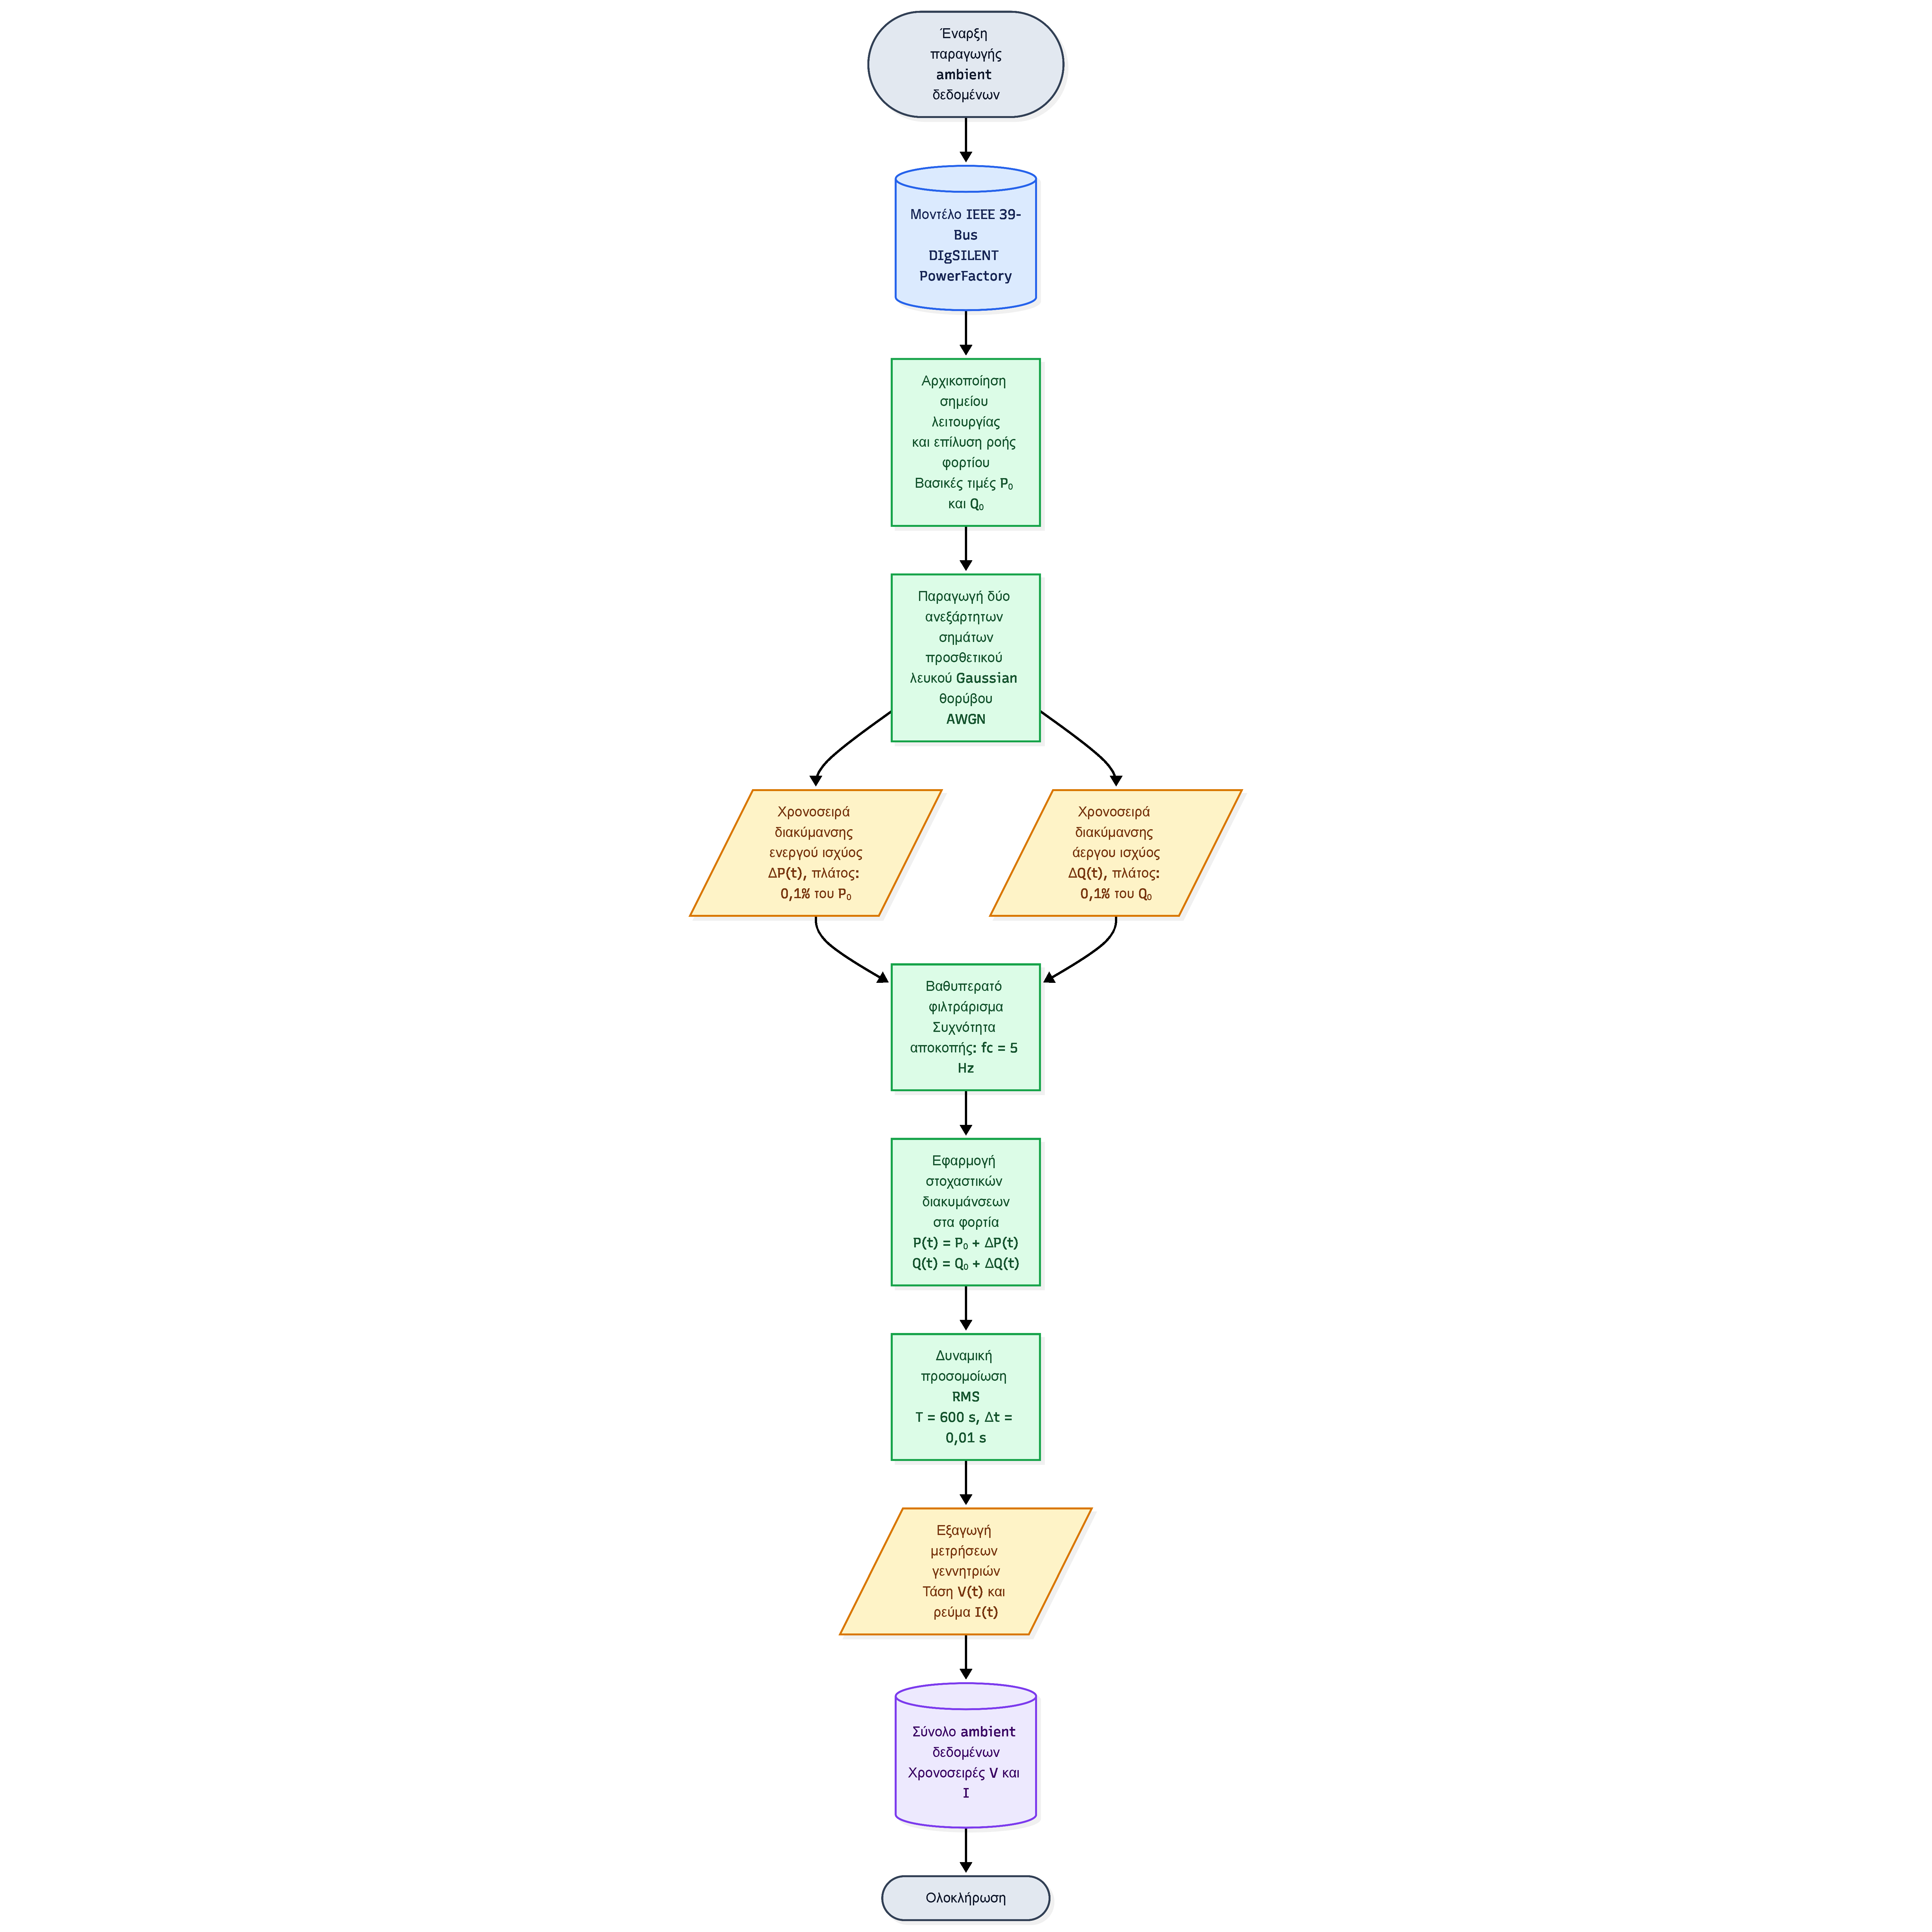
\includegraphics[width=0.72\textwidth,height=0.75\textheight,keepaspectratio,trim=900pt 0pt 900pt 0pt,clip]{images/ambient flowchart.pdf}
    \caption{Διάγραμμα ροής της διαδικασίας παραγωγής δεδομένων περιβαλλοντικών διακυμάνσεων (\textenglish{\textit{ambient}}) για το \textenglish{\textit{IEEE 39-Bus System}}.}
    \label{fig:amb:simulation-flowchart}
\end{figure}
\FloatBarrier

\section{Προεπεξεργασία Χρονοσειρών και Αλγόριθμος N4SID}
\label{amb:preprocessing}

 Στόχος της διαδικασίας ταυτοποίησης είναι η εκτίμηση των ηλεκτρομηχανικών ρυθμών του συστήματος από τις μετρήσεις ambient αποκρίσεων. Για τον σκοπό αυτό εφαρμόζεται ο αλγόριθμος ταυτοποίησης χώρου καταστάσεων \textenglish{\textit{N4SID}}~\cite{n4sid1994}, ο οποίος εκτιμά ένα διακριτό μοντέλο χώρου καταστάσεων και τις αντίστοιχες συχνότητες και αποσβέσεις των ρυθμών.

  Πριν από την εφαρμογή του αλγορίθμου, τα πρωτογενή δεδομένα υποβλήθηκαν σε \textenglish{\textit{detrending}}, υποδειγματοληψία στα $5$~Hz και βαθυπερατό φιλτράρισμα με συχνότητα αποκοπής $2$~Hz. Ο \textenglish{\textit{N4SID}} εφαρμόζεται επαναληπτικά σε δύο ομάδες τάξεων μοντέλου:
  \[
  n \in \{2,4,6,\dots,30\},
  \qquad
  n \in \{10,15,20,\dots,45\}.
  \]
  Μετά την ταυτοποίηση διατηρούνται μόνο οι εκτιμήσεις με συχνότητα στο διάστημα $[0.1,\,2.0]$~Hz και αρνητικό πραγματικό μέρος της ιδιοτιμής, δηλαδή ευσταθείς εκτιμήσεις, σύμφωνα με το εύρος των ηλεκτρομηχανικών ρυθμών του συστήματος~\cite{sarkar2024drga}.

\section{Προσδιορισμός Ρυθμών Αναφοράς από το PowerFactory}
\label{amb:reference_modes}

Εκτός από τις χρονοσειρές τάσης και ρεύματος, από το \textenglish{\textit{PowerFactory}} εξάγονται οι ιδιοτιμές αναφοράς για το ίδιο \textenglish{\textit{ambient}} σενάριο. Η διαδικασία περιλαμβάνει ανάλυση ιδιοτιμών, από την οποία διατηρούνται οι ιδιοτιμές που σχετίζονται με ηλεκτρομηχανικές ταλαντώσεις. Ο διαχωρισμός βασίζεται στον συντελεστή συμμετοχής ($p_{ki}$) των ιδιοτιμών στις καταστάσεις των σύγχρονων γεννητριών, που αφορούν τη γωνία δρομέα ($\delta$) και την ταχύτητα περιστροφής ($\omega$).

Για κάθε ρυθμό καταγράφονται η συχνότητα, η απόσβεση, οι γεννήτριες που συμμετέχουν και οι αντίστοιχες περιοχές ελέγχου. Διατηρούνται μόνο οι ρυθμοί με αρνητικό πραγματικό μέρος και θετικό φανταστικό μέρος. Το τελικό σύνολο αποτελεί την αναφορά για την αξιολόγηση των εκτιμήσεων N4SID και των αποτελεσμάτων της συσταδοποίησης.

\begin{table}[htbp]
    \centering
    \caption{Ηλεκτρομηχανικοί ρυθμοί αναφοράς που διατηρήθηκαν από το \textenglish{\textit{PowerFactory}}.}
    \label{tab:amb:pf_reference_modes}
    \begin{tabular}{cccccc}
        \toprule
        \textbf{ρυθμός ταλάντωσης} & \textbf{$f$ [Hz]} & \textbf{$\sigma$} & \textbf{γεννήτριες} & \textbf{περιοχές} & \textbf{τύπος} \\
        \midrule
        ρυθμός ταλάντωσης 1 & 1.110 & -0.193 & 8, 10& 1 & Intra-area \\
        ρυθμός ταλάντωσης 2 & 0.611 & -0.385 & 1, 5, 6, 9 & 1, 3 & Inter-area \\
        ρυθμός ταλάντωσης 3 & 1.049 & -0.399 & 1$-$7, 10 & 1$-$3 & Inter-area \\
        ρυθμός ταλάντωσης 4 & 0.968 & -0.464 & 5, 9 & 1, 3 & Inter-area \\
        ρυθμός ταλάντωσης 5 & 1.196 & -0.465 & 2, 3 & 2 & Intra-area \\
        ρυθμός ταλάντωσης 6 & 1.187 & -0.586 & 4$-$7 & 3 & Intra-area \\
        ρυθμός ταλάντωσης 7 & 1.423 & -0.696 & 6, 7 & 3 & Intra-area \\
        ρυθμός ταλάντωσης 8 & 1.410 & -0.710 & 8, 10 & 1 & Intra-area \\
        ρυθμός ταλάντωσης 9 & 1.451 & -0.817 & 4, 5 & 3 & Intra-area \\
        \bottomrule
    \end{tabular}
\end{table}

\section{Αλγόριθμοι Συσταδοποίησης και Βελτιστοποίηση Υπερπαραμέτρων}

Το σύνολο διατηρούμενων εκτιμήσεων ομαδοποιείται ανά περιοχή ελέγχου με τις μεθόδους \textenglish{\textit{k-Means}}~\cite{macqueen1967some}, \textenglish{\textit{k-Medoids}}~\cite{kaufman2009finding}, \textenglish{\textit{DBSCAN}}~\cite{dbscan1996}, \textenglish{\textit{OPTICS}}~\cite{optics1999}, \textenglish{\textit{HDBSCAN}}~\cite{hdbscan2015}, \textenglish{GMM}~\cite{gmm2002} και AHC~\cite{agglomerative1963}. Οι παράμετροι κάθε μεθόδου και η μεθοδολογία επιλογής τους παρουσιάζονται σε επόμενη ενότητα μαζί με τα αποτελέσματα, ώστε η σύγκριση να βασίζεται σε κοινό σύνολο δεδομένων εισόδου και σαφώς ορισμένες ρυθμίσεις.

\subsection{Διαδικασία Ρύθμισης Υπερπαραμέτρων}
\label{amb:clustering-tuning}
Η ρύθμιση των υπερπαραμέτρων των αλγορίθμων συσταδοποίησης πραγματοποιήθηκε ανεξάρτητα για κάθε συνδυασμό σάρωσης τάξεων μοντέλου και περιοχής ελέγχου,
χρησιμοποιώντας το αντίστοιχο σύνολο διατηρούμενων εκτιμήσεων που προέκυψε από τον N4SID. Για τις μεθόδους που απαιτούν εκ των προτέρων
καθορισμό αριθμού συστάδων (\textenglish{\textit{k-Means}}, \textenglish{\textit{k-Medoids}} και \textenglish{\textit{GMM}}) ή κατωφλίου γειτνίασης (\textenglish{\textit{DBSCAN}}, \textenglish{\textit{HDBSCAN}} και AHC), εξετάστηκε ένα προκαθορισμένο σύνολο υποψήφιων τιμών. Η τελική επιλογή των υπερπαραμέτρων έγινε με βάση τη μεγιστοποίηση του δείκτη \textenglish{\textit{silhouette score}} για όλους τους αλγορίθμους συσταδοποίησης, με μοναδική εξαίρεση τον GMM για τον οποίο επιλέχθηκε η παραμετροποίηση που ελαχιστοποιεί το κριτήριο BIC.

Η συσταδοποίηση εφαρμόστηκε στις συντεταγμένες των πόλων
\[
\mathbf{X}=[\sigma,\omega],
\qquad
\omega=2\pi f,
\]
όπου η απόσβεση $\sigma$ και η γωνιακή συχνότητα $\omega$ εκφράζονται
σε rad/s. Οι ίδιες συντεταγμένες χρησιμοποιήθηκαν για την εφαρμογή των
αλγορίθμων, τον υπολογισμό των αποστάσεων και την αξιολόγηση των
υποψήφιων υπερπαραμέτρων. Οι χάρτες ρυθμών παρουσιάζονται στο ισοδύναμο επίπεδο
$(\sigma,f)$, ώστε η συχνότητα να εκφράζεται σε Hz για λόγους αναγνωσιμότητας.

Για τις μεθόδους πυκνότητας (\textenglish{\textit{DBSCAN}}, \textenglish{\textit{OPTICS}} και
\textenglish{\textit{HDBSCAN}}), το $N_{\mathrm{pts}}$ και, ειδικά για τους \textenglish{\textit{DBSCAN}} και \textenglish{\textit{HDBSCAN}}, η παράμετρος $\epsilon$
υπολογίστηκαν σύμφωνα με τη διαδικασία της
\cite{sfetkos2024measurement}:
\begin{equation}
\epsilon =
\frac{p_e}{2}
\sqrt{(\sigma_{\max}-\sigma_{\min})^2+
    (\omega_{\max}-\omega_{\min})^2}.
\label{eq:amb:epsilon-scaling}
\end{equation}
\begin{equation}
N_{\mathrm{pts}}=
\max\left(2,\left\lceil p_m N_s|n|\right\rceil\right).
\label{eq:amb:npts-scaling}
\end{equation}
όπου $N_s$ είναι το πλήθος των συνδυασμών γεννήτριας$-$σήματος στην
εξεταζόμενη περιοχή ελέγχου και $|n|$ το πλήθος των τάξεων μοντέλου του
αντίστοιχου sweep. Οι συντελεστές $p_e$ και $p_m$ δεν αποτελούν άμεσες
υπερπαραμέτρους των αλγορίθμων, αλλά χρησιμοποιούνται για τον προσαρμοστικό
υπολογισμό των αντίστοιχων ρυθμίσεων με βάση το εύρος και το πλήθος των
διαθέσιμων εκτιμήσεων. Ειδικότερα, μέσω της~\eqref{eq:amb:epsilon-scaling},
ο $p_e$ καθορίζει την τιμή της $\epsilon$, η οποία χρησιμοποιείται ως
\texttt{eps} στον \textenglish{\textit{DBSCAN}}, ως
\texttt{cluster\_selection\_epsilon} στον \textenglish{\textit{HDBSCAN}}
και ως \texttt{distance\_threshold} στην AHC. Αντίστοιχα, μέσω
της~\eqref{eq:amb:npts-scaling}, ο $p_m$ καθορίζει το $N_{\mathrm{pts}}$,
το οποίο χρησιμοποιείται ως \texttt{min\_samples} στους
\textenglish{\textit{DBSCAN}} και \textenglish{\textit{OPTICS}} και ως
\texttt{min\_cluster\_size} στον \textenglish{\textit{HDBSCAN}}.

Τα πλέγματα υπερπαραμέτρων που χρησιμοποιήθηκαν
παρουσιάζονται συγκεντρωτικά στον Πίνακα~\ref{tab:amb:hyperparameter-grids},
όπου $N$ είναι το πλήθος των διαθέσιμων διατηρούμενων εκτιμήσεων. Τα ίδια
πλέγματα εφαρμόστηκαν και στις δύο σαρώσεις τάξεων μοντέλου.

\begin{table}[htbp]
    \centering
    \caption{Πλέγματα υπερπαραμέτρων των μεθόδων συσταδοποίησης.}
    \label{tab:amb:hyperparameter-grids}
    \footnotesize
    \setlength{\tabcolsep}{5pt}
    \renewcommand{\arraystretch}{1.35}
    \begin{tabular}{
        >{\raggedright\arraybackslash}p{0.18\textwidth}
        >{\raggedright\arraybackslash}p{0.37\textwidth}
        >{\raggedright\arraybackslash}p{0.34\textwidth}}
        \toprule
        \textbf{Μέθοδος} & \textbf{Πλέγμα αναζήτησης} & \textbf{Σταθερές ρυθμίσεις} \\
        \midrule
        \textenglish{\textit{k-Means}}, \textenglish{\textit{k-Medoids}}
        & $K\in\{2,3,\ldots,\min(10,N-1)\}$
        & --- \\
        \textenglish{\textit{DBSCAN}}
        & $p_e\in\{0.060,0.065,\ldots,0.150\}$\newline
          $p_m\in\{0.10,0.15,\ldots,0.35\}$
        & --- \\
        \textenglish{\textit{OPTICS}}
        & $p_m\in\{0.30,0.35,0.40\}$\newline
          $\xi\in\{0.02,0.03,0.04,0.05,0.06\}$
        & \texttt{min\_samples}$=N_{\mathrm{pts}}$ \\
        \textenglish{\textit{HDBSCAN}}
        & $p_e\in\{0.010,0.015,\ldots,0.150\}$\newline
          $p_m\in\{0.10,0.15,\ldots,0.40\}$
        & \texttt{min\_cluster\_size}$=N_{\mathrm{pts}}$;\newline
          \texttt{cluster\_selection\_epsilon}$=\epsilon$;\newline
          \texttt{cluster\_selection\_method}$\in\{\texttt{eom},\texttt{leaf}\}$ \\
        \textenglish{\textit{GMM}}
        & $K\in\{1,2,\ldots,\min(10,N)\}$
        & \texttt{covariance\_type}$=\texttt{full}$;\newline
          \texttt{reg\_covar}$=10^{-4}$;\newline
          \texttt{n\_init}$=10$;\newline
          αρχικοποίηση \textit{k-means++} \\
        \textenglish{\textit{Agglomerative}}
        & $p_e\in\{0.01,0.02,\ldots,0.80\}$
        & \texttt{linkage}$\in\{\textenglish{\textit{average}},\textenglish{\textit{complete}}\}$ \\
        \bottomrule
    \end{tabular}
\end{table}

Μία υποψήφια ρύθμιση θεωρήθηκε έγκυρη για την αξιολόγηση με silhouette
μόνο όταν παρήγαγε τουλάχιστον δύο συστάδες που δεν αντιστοιχούν σε θόρυβο.

\subsection{Φιλτράρισμα Συστάδων βάσει Silhouette Score}
\label{amb:silhouette-filtering}
Οι μέθοδοι k-Means, k-Medoids, GMM και AHC αποδίδουν κάθε εκτίμηση σε μία συστάδα και δεν διαθέτουν κάποιον μηχανισμό για την αναγνώριση εκτιμήσεων ως θόρυβο. Για αυτές τις μεθόδους λοιπόν εφαρμόστηκε, μετά την επιλογή των υπερπαραμέτρων, φιλτράρισμα των συστάδων με βάση τον δείκτη Silhouette Score. Συγκεκριμένα, για κάθε συστάδα υπολογίστηκε το μέσο Silhouette Score των εκτιμήσεων που περιείχε και συστάδες με μέσο Silhouette Score μικρότερο του $0.25$ απορρίφθηκαν ως θόρυβος.

\section{Μετρικές Αξιολόγησης}

Για την αξιολόγηση των αποτελεσμάτων, κάθε εκτιμώμενος ρυθμός αντιστοιχίζεται αρχικά στον πλησιέστερο σχετικό ηλεκτρομηχανικό ρυθμό αναφοράς του \textenglish{\textit{PowerFactory}} στο επίπεδο $(\sigma,\omega)$. Η αντιστοίχιση αυτή χρησιμοποιείται ως βάση σύγκρισης με τις συστάδες που προκύπτουν από τις μεθόδους συσταδοποίησης.

Οι μετρικές \textenglish{\textit{V-measure}} και ARI αξιολογούν τον βαθμό συμφωνίας μεταξύ
των συστάδων που προκύπτουν από κάθε μέθοδο και της παραπάνω αντιστοίχισης
στους ρυθμούς αναφοράς. Επομένως, εκφράζουν κατά πόσο η μέθοδος διαχωρίζει
τις εκτιμήσεις που αντιστοιχούν σε διαφορετικούς ηλεκτρομηχανικούς ρυθμούς.

Συμπληρωματικά, ο MAD υπολογίζεται για κάθε μέθοδο και για κάθε ρυθμό
αναφοράς. Εκφράζει τη διάμεση απόκλιση των εκτιμήσεων που αποδίδονται στον
συγκεκριμένο ρυθμό από την αντίστοιχη ιδιοτιμή αναφοράς, ως προς το
πραγματικό και το φανταστικό μέρος της ιδιοτιμής, δηλαδή στο επίπεδο
$(\sigma,\omega)$. Μικρότερες τιμές MAD υποδηλώνουν ακριβέστερη εκτίμηση του
αντίστοιχου ρυθμού.

\chapter{Αποτελέσματα Ταυτοποίησης και Συγκριτική Αξιολόγηση Αλγορίθμων Συσταδοποίησης}

\section{Διατηρούμενες Εκτιμήσεις (\textenglish{Screened Estimates})}

Με βάση τα κριτήρια screening της Ενότητας~\ref{amb:preprocessing}, το πρώτο sweep τάξεων, $n \in \{2,4,\dots,30\}$, αποδίδει 1397 εκτιμήσεις, ενώ το δεύτερο sweep τάξεων, $n \in \{10,15,\dots,45\}$, αποδίδει 1391 εκτιμήσεις. Η κατανομή τους ανά περιοχή ελέγχου και ο χρόνος εκτέλεσης του N4SID παρουσιάζονται στον Πίνακα~\ref{tab:amb:screened_estimates}.

\begin{table}[htbp]
    \centering
    \caption{Πλήθος διατηρούμενων εκτιμήσεων και χρόνος εκτέλεσης N4SID ανά σάρωση τάξεων μοντέλου και περιοχή ελέγχου.}
    \label{tab:amb:screened_estimates}
    \resizebox{\textwidth}{!}{%
    \begin{tabular}{cccccc}
        \toprule
        \textbf{σάρωση τάξεων μοντέλου} & \textbf{Περιοχή 1} & \textbf{Περιοχή 2} & \textbf{Περιοχή 3} & \textbf{Σύνολο} & \makecell{\textbf{Χρόνος N4SID}\\\textbf{[s]}} \\
        \midrule
        $n \in \{2,4,\dots,30\}$ & 565 & 280 & 552 & 1397 & 3.1 \\
        $n \in \{10,15,\dots,45\}$ & 548 & 272 & 571 & 1391 & 2.9 \\
        \bottomrule
    \end{tabular}
    }
\end{table}

Το Σχήμα~\ref{fig:amb:screened_modal_grid} απεικονίζει τις διατηρούμενες εκτιμήσεις στο επίπεδο $(\sigma,f)$, ανά σάρωση τάξεων μοντέλου και περιοχή ελέγχου. Τα κοινά όρια των αξόνων επιτρέπουν την άμεση οπτική σύγκριση των συγκεντρώσεων, ενώ οι δείκτες αναφοράς αντιστοιχούν στους ρυθμούς του \textenglish{\textit{PowerFactory}} του Πίνακα~\ref{tab:amb:pf_reference_modes}.

Τα συγκρίσιμα συνολικά πλήθη των δύο σαρώσεων δείχνουν ότι η μεταβολή του εύρους των τάξεων μοντέλου δεν αλλάζει ουσιαστικά τον αριθμό των εκτιμήσεων που ικανοποιούν τα κριτήρια διαλογής. Οι μικρές διαφοροποιήσεις ανά περιοχή οφείλονται στο διαφορετικό πλήθος πόλων που ανακτάται για κάθε συνδυασμό τάξης μοντέλου, γεννήτριας και μετρούμενου μεγέθους. Επομένως, οι δύο σαρώσεις παρέχουν σύνολα παρόμοιου μεγέθους και μπορούν να συγκριθούν χωρίς σημαντική ανισορροπία δείγματος.

Η κοινή απεικόνιση των έξι συνδυασμών επιτρέπει επιπλέον να εξεταστεί αν οι συγκεντρώσεις παραμένουν σταθερές όταν αλλάζει η σάρωση τάξεων. Η σύγκριση γίνεται πρωτίστως ως προς τη συχνότητα, όπου αναμένονται συγκεντρώσεις κοντά στους ρυθμούς αναφοράς, και δευτερευόντως ως προς την απόσβεση, όπου η διασπορά των εκτιμήσεων είναι εντονότερη.

\clearpage
\begin{figure}[H]
    \centering
    \includegraphics[width=\textwidth,height=0.86\textheight,keepaspectratio]{\ambientfigurepath Ambient_Mag0.1_T600s_dt10ms_seed1997/plots/pdf/screened_modal_maps_3x2_grid.pdf}
    \caption{Διατηρούμενες εκτιμήσεις N4SID στο επίπεδο $(\sigma,f)$ ανά σάρωση τάξεων μοντέλου και περιοχή ελέγχου. Οι χρωματισμοί διακρίνουν τα σήματα τάσης και ρεύματος, ενώ οι λευκοί ρόμβοι δηλώνουν τους ρυθμούς αναφοράς του \textenglish{\textit{PowerFactory}} του Πίνακα~\ref{tab:amb:pf_reference_modes}.}
    \label{fig:amb:screened_modal_grid}
\end{figure}

Είναι εμφανές ότι οι δύο σαρώσεις τάξεων μοντέλου εμφανίζουν παρόμοια κατανομή των εκτιμήσεων και στις τρεις περιοχές ελέγχου, καθώς και ότι οι εκτιμήσεις του N4SID συγκεντρώνονται κοντά στις συχνότητες των ρυθμών αναφοράς του \textenglish{\textit{PowerFactory}}, επομένως η μέθοδος αποδίδει ικανοποιητικά τη θέση των ηλεκτρομηχανικών ρυθμών ως προς τη συχνότητα $f$. Αντίθετα, παρατηρείται μεγαλύτερη διασπορά κατά τον άξονα της απόσβεσης $\sigma$. Η διασπορά αυτή αναδεικνύει ότι η εκτίμηση της απόσβεσης είναι λιγότερο σταθερή από την εκτίμηση της συχνότητας και αιτιολογεί την επόμενη εφαρμογή συσταδοποίησης.


\section{Αποτελέσματα Συσταδοποίησης ανά Μέθοδο}
\label{sec:amb:clustering-by-method}

Η παρούσα ενότητα παρουσιάζει, για κάθε αλγόριθμο, τις ρυθμίσεις που
επιλέχθηκαν από τη διαδικασία ρύθμισης υπερπαραμέτρων της Ενότητας~\ref{amb:clustering-tuning}.
Οι πίνακες συνοψίζουν τις επιλεγμένες ρυθμίσεις για κάθε σάρωση τάξεων μοντέλου και
περιοχή ελέγχου. Η ερμηνεία των αποτελεσμάτων βασίζεται στο πλήθος των
συστάδων, στον χειρισμό του θορύβου και στο \textenglish{\textit{silhouette score}}, ενώ η
άμεση σύγκριση όλων των μεθόδων ακολουθεί στην επόμενη ενότητα.

Για τις μεθόδους \textenglish{\textit{DBSCAN}}, \textenglish{\textit{OPTICS}} και \textenglish{\textit{HDBSCAN}}, ως θόρυβος χαρακτηρίζονται οι εκτιμήσεις που δεν εντάσσονται από τον ίδιο τον αλγόριθμο σε κάποια συστάδα. Στους αντίστοιχους πίνακες, το ποσοστό θορύβου εκφράζει το ποσοστό αυτών των εκτιμήσεων επί του συνολικού πλήθους εκτιμήσεων εισόδου.

\subsection{k-Means}

Για τον \textenglish{\textit{k-Means}}, η επιλογή του αριθμού συστάδων βασίστηκε στη
μέγιστη τιμή silhouette και στο φιλτράρισμα της Ενότητας~\ref{amb:silhouette-filtering}. Οι επιλεγμένες λύσεις περιλαμβάνουν από δύο έως
πέντε συστάδες και όλα τα σημεία αποδίδονται σε κάποια συστάδα καθώς ο αλγόριθμος δεν κάνει διαχωρισμό των σημείων σε θόρυβο αλλά και καμία συστάδα δεν προέκυψε με μέσο silhouette score μικρότερο του 0.25. Όλες οι τιμές των Silhouette Score είναι παρόμοιες, γεγονός που υποδηλώνει παρόμοια συνοχή των συστάδων σε όλες τις περιοχές ελέγχου με τις τιμές στην Περιοχή 2 να είναι ελαφρώς υψηλότερες και στις δύο σαρώσεις τάξεων μοντέλου. Οι επιλεγμένες τιμές του \textit{k} παρουσιάζονται στον Πίνακα~\ref{tab:amb:kmeans-tuning}.

\begin{table}[htbp]
    \centering
    \caption{Επιλεγμένες ρυθμίσεις \textenglish{\textit{k-Means}}.}
    \label{tab:amb:kmeans-tuning}
    \begin{tabular}{cccc}
        \toprule
        Sweep & Περιοχή & $k$ & Silhouette Score \\
        \midrule
        Ομάδα τάξεων 1 & 1 & 5 & 0.640 \\
        Ομάδα τάξεων 1 & 2 & 4 & 0.700 \\
        Ομάδα τάξεων 1 & 3 & 4 & 0.650 \\
        Ομάδα τάξεων 2 & 1 & 2 & 0.609 \\
        Ομάδα τάξεων 2 & 2 & 5 & 0.681 \\
        Ομάδα τάξεων 2 & 3 & 2 & 0.621 \\
        \bottomrule
    \end{tabular}
\end{table}

\subsection{k-Medoids}

Ο \textenglish{\textit{k-Medoids}} ρυθμίστηκε με το ίδιο εύρος τιμών $K$ και το ίδιο
κριτήριο επιλογής με τον \textenglish{\textit{k-Means}} όπως περιγράφηκε στην Ενότητα~\ref{amb:clustering-tuning}. Παρατηρείται ότι οι περισσότερες επιλεγμένες τιμές του $k$ είναι ίδιες με αυτές του \textenglish{\textit{k-Means}}, ενώ εξαιρετική ομοιότητα παρατηρείται και στις τιμές του silhouette score. Όμοια με τον k-Means, δεν προέκυψε καμία συστάδα με Silhouette Score μικρότερο του 0.25 οπότε δεν χαρακτηρίζεται καμία εκτίμηση ως θόρυβος. Οι επιλεγμένες τιμές του \textit{k} παρουσιάζονται στον Πίνακα~\ref{tab:amb:kmedoids-tuning}.

\begin{table}[htbp]
    \centering
    \caption{Επιλεγμένες ρυθμίσεις \textenglish{\textit{k-Medoids}}.}
    \label{tab:amb:kmedoids-tuning}
    \begin{tabular}{cccc}
        \toprule
        Sweep & Περιοχή & $k$ & Silhouette Score \\
        \midrule
        Ομάδα τάξεων 1 & 1 & 5 & 0.634 \\
        Ομάδα τάξεων 1 & 2 & 4 & 0.702 \\
        Ομάδα τάξεων 1 & 3 & 4 & 0.654 \\
        Ομάδα τάξεων 2 & 1 & 2 & 0.609 \\
        Ομάδα τάξεων 2 & 2 & 4 & 0.664 \\
        Ομάδα τάξεων 2 & 3 & 4 & 0.621 \\
        \bottomrule
    \end{tabular}
\end{table}

\subsection{DBSCAN}

Ο DBSCAN επέλεξε σε όλες τις περιπτώσεις την ελάχιστη τιμή της παραμέτρου $p_e$ ($p_e = 0.060$). Ωστόσο, δεν κρίνεται σκόπιμο να μειωθεί το κατώφλι $p_e$, καθώς θα αυξανόταν περαιτέρω το ποσοστό των εκτιμήσεων που χαρακτηρίζονται ως θόρυβος. Ακόμα, η μέθοδος παρήγαγε από τρεις έως έξι συστάδες σε κάθε περίπτωση με σχετικά υψηλά silhouette scores, γεγονός που υποδηλώνει πολύ συνεκτικές συστάδες, με μειονέκτημα όμως την απόρριψη σημαντικού μέρους των εκτιμήσεων ως θόρυβο. Οι επιλεγμένες τιμές των υπερπαραμέτρων παρουσιάζονται στον Πίνακα~\ref{tab:amb:dbscan-tuning}.

\begin{table}[htbp]
    \centering
    \caption{Επιλεγμένες ρυθμίσεις DBSCAN.}
    \label{tab:amb:dbscan-tuning}
    \resizebox{\textwidth}{!}{%
    \begin{tabular}{cccccccc}
        \toprule
        Sweep & Περιοχή & $p_e$ & $p_m$ & $N_{\mathrm{pts}}$ & συστάδες & θόρυβος [\%] & Silhouette \\
        \midrule
        Ομάδα τάξεων 1 & 1 & 0.060 & 0.35 & 42 & 4 & 36.8 & 0.837 \\
        Ομάδα τάξεων 1 & 2 & 0.060 & 0.35 & 21 & 4 & 36.4 & 0.856 \\
        Ομάδα τάξεων 1 & 3 & 0.060 & 0.35 & 42 & 3 & 50.2 & 0.885 \\
        Ομάδα τάξεων 2 & 1 & 0.060 & 0.35 & 23 & 6 & 25.4 & 0.641 \\
        Ομάδα τάξεων 2 & 2 & 0.060 & 0.35 & 12 & 4 & 21.3 & 0.774 \\
        Ομάδα τάξεων 2 & 3 & 0.060 & 0.35 & 23 & 5 & 24.2 & 0.697 \\
        \bottomrule
    \end{tabular}
    }
\end{table}

\subsection{OPTICS}

Ο αλγόριθμος OPTICS επέλεξε από τέσσερις έως οκτώ συστάδες στις εξεταζόμενες περιπτώσεις, με επίσης υψηλά silhouette scores. Όμως, όπως
και στον DBSCAN, οι υψηλές τιμές silhouette συνοδεύονται από χαρακτηρισμό σημαντικού ποσοστού
σημείων ως θόρυβο. Επομένως, οι ρυθμίσεις με τη μεγαλύτερη τιμή silhouette
περιγράφουν συνεκτικές ομάδες εκτιμήσεων, χωρίς όμως να καλύπτουν το
σύνολο του διαθέσιμου δείγματος. Οι επιλεγμένες τιμές των υπερπαραμέτρων παρουσιάζονται στον Πίνακα~\ref{tab:amb:optics-tuning}.

\begin{table}[htbp]
    \centering
    \caption{Επιλεγμένες ρυθμίσεις OPTICS.}
    \label{tab:amb:optics-tuning}
    \resizebox{\textwidth}{!}{%
    \begin{tabular}{cccccccc}
        \toprule
        Sweep & Περιοχή & $p_m$ & \texttt{xi} & \texttt{min\_samples} & συστάδες & θόρυβος [\%] & Silhouette \\
        \midrule
        Ομάδα τάξεων 1 & 1 & 0.40 & 0.03 & 48 & 4 & 30.6 & 0.768 \\
        Ομάδα τάξεων 1 & 2 & 0.30 & 0.05 & 18 & 5 & 20.7 & 0.783 \\
        Ομάδα τάξεων 1 & 3 & 0.35 & 0.03 & 42 & 4 & 38.6 & 0.808 \\
        Ομάδα τάξεων 2 & 1 & 0.35 & 0.06 & 23 & 8 & 30.1 & 0.710 \\
        Ομάδα τάξεων 2 & 2 & 0.40 & 0.05 & 13 & 7 & 29.4 & 0.776 \\
        Ομάδα τάξεων 2 & 3 & 0.40 & 0.06 & 26 & 6 & 53.1 & 0.804 \\
        \bottomrule
    \end{tabular}
    }
\end{table}

\subsection{HDBSCAN}

Ο HDBSCAN διατηρεί πολύ μεγαλύτερο μέρος των εκτιμήσεων σε σχέση με τις δύο
προηγούμενες density-based μεθόδους, επιλέγοντας όμως από τέσσερις έως εννέα
συστάδες. Οι τιμές silhouette παραμένουν υψηλές σε όλες τις περιοχές. Οπτικά η μέθοδος φαίνεται να ανακτά όλες τις βασικές διακριτές συγκεντρώσεις των εκτιμήσεων στο επίπεδο $(\sigma,f)$ ενώ παράλληλα απορρίπτει ως θόρυβο τις εκτιμήσεις που δεν ανήκουν σε πυκνές περιοχές. Η μέθοδος \texttt{eom} επιλέχθηκε σε όλες τις περιπτώσεις, με μοναδική εξαίρεση το δεύτερο sweep της Περιοχής 3, όπου επιλέχθηκε η πολιτική \texttt{leaf}. Οι επιλεγμένες τιμές των υπερπαραμέτρων παρουσιάζονται στον Πίνακα~\ref{tab:amb:hdbscan-tuning}.

\begin{table}[htbp]
    \centering
    \caption{Επιλεγμένες ρυθμίσεις HDBSCAN.}
    \label{tab:amb:hdbscan-tuning}
    \resizebox{\textwidth}{!}{%
    \begin{tabular}{ccccccccc}
        \toprule
        Sweep & Περιοχή & $p_e$ & $p_m$ & \texttt{min\_cluster\_size} & μέθοδος & συστάδες & θόρυβος [\%] & Silhouette \\
        \midrule
        Ομάδα τάξεων 1 & 1 & 0.010 & 0.35 & 42 & eom & 4 & 29.2 & 0.796 \\
        Ομάδα τάξεων 1 & 2 & 0.010 & 0.20 & 12 & eom & 7 & 21.4 & 0.782 \\
        Ομάδα τάξεων 1 & 3 & 0.010 & 0.20 & 24 & eom & 5 & 25.4 & 0.816 \\
        Ομάδα τάξεων 2 & 1 & 0.010 & 0.30 & 20 & eom & 9 & 34.1 & 0.741 \\
        Ομάδα τάξεων 2 & 2 & 0.065 & 0.40 & 13 & eom & 4 & 12.5 & 0.749 \\
        Ομάδα τάξεων 2 & 3 & 0.010 & 0.40 & 26 & leaf & 6 & 39.2 & 0.742 \\
        \bottomrule
    \end{tabular}
    }
\end{table}

\subsection{Gaussian Mixture Models}

Για τον GMM, οι υπερπαράμετροι επιλέχθηκαν με κριτήριο την
ελαχιστοποίηση του BIC και όχι με βάση το silhouette Score όπως στις υπόλοιπες μεθόδους. Η αρχική λύση
επιλέγει εννέα ή δέκα Gaussian συνιστώσες/συστάδες σε κάθε περίπτωση και αποδίδει όλες τις εκτιμήσεις
σε κάποια συνιστώσα/συστάδα. Στη συνέχεια όμως το φίλτρο της Ενότητας~\ref{amb:silhouette-filtering} απορρίπτει ως θόρυβο έως και πέντε από τις αρχικές συστάδες. Τελικά, οπτικά φαίνεται να ανακτά όλες τις εμφανείς συγκεντρώσεις εκτιμήσεων παρόμοια με τον HDBSCAN. Οι αντίστοιχες τιμές Silhouette πριν και μετά το φιλτράρισμα παρουσιάζονται μόνο συμπληρωματικά και δεν αποτελούν κριτήριο επιλογής του μοντέλου. Οι επιλεγμένες τιμές των υπερπαραμέτρων, οι συστάδες και τα Silhouette Score παρουσιάζονται στον Πίνακα~\ref{tab:amb:gmm-tuning}.

\begin{table}[htbp]
    \centering
    \caption{Επιλεγμένες ρυθμίσεις GMM.}
    \label{tab:amb:gmm-tuning}
    \resizebox{\textwidth}{!}{%
    \begin{tabular}{ccccccc}
        \toprule
        Sweep & Περιοχή & $k$ & BIC & \makecell{Silhouette\\(ρύθμιση υπερπαραμέτρων)} & \makecell{Τελικές\\συστάδες} & \makecell{Τελικό\\silhouette}\\
        \midrule
        Ομάδα τάξεων 1 & 1 & 10 & 2465.84 & 0.363 & 7 & 0.621 \\
        Ομάδα τάξεων 1 & 2 & 10 & 959.29 & 0.454 & 7 & 0.734 \\
        Ομάδα τάξεων 1 & 3 & 10 & 2337.83 & 0.374 & 6 & 0.718 \\
        Ομάδα τάξεων 2 & 1 & 10 & 2340.35 & 0.083 & 6 & 0.705 \\
        Ομάδα τάξεων 2 & 2 & 10 & 1142.22 & 0.497 & 8 & 0.587 \\
        Ομάδα τάξεων 2 & 3 & 9 & 2559.48 & 0.143 & 4 & 0.821 \\
        \bottomrule
    \end{tabular}
    }
\end{table}

\subsection{Agglomerative Hierarchical Clustering}

Η AHC αρχικά επίσης αποδίδει όλες τις εκτιμήσεις σε
συστάδες, χωρίς χαρακτηρισμό σημείων ως θορύβου. Οι ρυθμίσεις που
μεγιστοποιούν το silhouette οδηγούν σε τρεις έως επτά συστάδες, σε δύο όμως περιπτώσεις η μετεπεξεργασία της Ενότητας~\ref{amb:silhouette-filtering} αφαιρεί συστάδες χαμηλής συνοχής. Οι επιλεγμένες τιμές των υπερπαραμέτρων καθώς και ο αρχικός και τελικός αριθμός συστάδων καθώς και τα αντίστοιχα Silhouette Score παρουσιάζονται στον Πίνακα~\ref{tab:amb:agglomerative-tuning}.

\begin{table}[htbp]
    \centering
    \caption{Επιλεγμένες ρυθμίσεις AHC.}
    \label{tab:amb:agglomerative-tuning}
    \resizebox{\textwidth}{!}{%
    \begin{tabular}{cccccccc}
        \toprule
        Sweep & Περιοχή & $p_e$ & Linkage & \makecell{συστάδες\\(ρύθμιση υπερπαραμέτρων)} & \makecell{Silhouette\\(ρύθμιση υπερπαραμέτρων)} & \makecell{Τελικές\\συστάδες} & \makecell{Τελικό\\silhouette} \\
        \midrule
        Ομάδα τάξεων 1 & 1 & 0.36 & average & 7 & 0.626 & 5 & 0.633 \\
        Ομάδα τάξεων 1 & 2 & 0.54 & complete & 4 & 0.685 & 4 & 0.685 \\
        Ομάδα τάξεων 1 & 3 & 0.73 & complete & 6 & 0.633 & 6 & 0.633 \\
        Ομάδα τάξεων 2 & 1 & 0.79 & average & 3 & 0.569 & 2 & 0.587 \\
        Ομάδα τάξεων 2 & 2 & 0.49 & average & 4 & 0.670 & 4 & 0.670 \\
        Ομάδα τάξεων 2 & 3 & 0.67 & complete & 6 & 0.607 & 6 & 0.607 \\
        \bottomrule
    \end{tabular}
    }
\end{table}


\section{Συγκριτική Αξιολόγηση των Αποτελεσμάτων των Μεθόδων Συσταδοποίησης}

Η διαδικασία ρύθμισης υπερπαραμέτρων οδηγεί σε διαφορετικό πλήθος συστάδων, ανάλογα με τη
μέθοδο, την περιοχή ελέγχου και τη σάρωση τάξεων μοντέλου. Το πλήθος αυτό αποτελεί
χρήσιμη πρώτη ένδειξη της συμπεριφοράς κάθε μεθόδου: πολύ μικρές τιμές
ενδέχεται να συγχωνεύουν ξεχωριστές modal συγκεντρώσεις, ενώ πολύ μεγάλες
τιμές μπορεί να υποδεικνύουν υπερκατατμημένη περιγραφή των εκτιμήσεων.

Ο Πίνακας~\ref{tab:amb:clustering-comparison} συγκεντρώνει το επιλεγμένο
πλήθος συστάδων ανά σάρωση τάξεων μοντέλου και περιοχή ελέγχου. Παρουσιάζεται επίσης
το πλήθος των ρυθμών αναφοράς του \textenglish{\textit{PowerFactory}} που σχετίζονται με
κάθε περιοχή, σύμφωνα με τον Πίνακα~\ref{tab:amb:pf_reference_modes}. Οι
αναλυτικές ρυθμίσεις που οδήγησαν στις συγκεκριμένες επιλογές παρουσιάστηκαν
στην Ενότητα~\ref{sec:amb:clustering-by-method}.

\clearpage
\begin{landscape}
\vspace*{0.06\textheight}
\noindent\begin{minipage}{0.98\linewidth}
Ο Πίνακας~\ref{tab:amb:clustering-comparison} επιτρέπει την άμεση σύγκριση του πλήθους συστάδων που επιλέγει κάθε μέθοδος με το αντίστοιχο πλήθος ρυθμών αναφοράς. Τιμές μικρότερες από το αναμενόμενο υποδεικνύουν πιθανή συγχώνευση κοντινών ρυθμών, ενώ σημαντικά μεγαλύτερες τιμές αποτελούν ένδειξη υπερκατάτμησης των εκτιμήσεων. Η σύγκριση πραγματοποιείται χωριστά για τις δύο σαρώσεις τάξεων μοντέλου και για καθεμία από τις τρεις περιοχές ελέγχου.
\end{minipage}
\vspace{1.5em}
\begin{table}[H]
    \centering
    \caption{Πλήθος συστάδων της επιλεγμένης ρύθμισης ανά σάρωση τάξεων μοντέλου, περιοχή ελέγχου και μέθοδο.}
    \label{tab:amb:clustering-comparison}
    \resizebox{0.98\linewidth}{!}{%
    \begin{tabular}{ccc|ccccccc}
        \toprule
        \textbf{Sweep} & \textbf{Περ.} & \shortstack{\\\textbf{Ρυθμοί αναφοράς}} & \shortstack{\textbf{k-}\\\textbf{Means}} & \shortstack{\textbf{k-}\\\textbf{Medoids}} & \textbf{DBSCAN} & \textbf{OPTICS} & \textbf{HDBSCAN} & \textbf{GMM} & \textbf{AHC} \\
        \midrule
        \multirow{3}{*}{Ομάδα τάξεων 1} & 1 & 5 & 5 & 5 & 4 & 4 & 4 & 7 & 5 \\
        & 2 & 2 & 4 & 4 & 4 & 5 & 7 & 7 & 4 \\
        & 3 & 5 & 4 & 4 & 3 & 4 & 5 & 6 & 6 \\
        \midrule
        \multirow{3}{*}{Ομάδα τάξεων 2} & 1 & 5 & 2 & 2 & 6 & 8 & 9 & 6 & 2 \\
        & 2 & 2 & 5 & 4 & 4 & 7 & 4 & 8 & 4 \\
        & 3 & 5 & 2 & 4 & 5 & 6 & 6 & 4 & 6 \\
        \bottomrule
    \end{tabular}
    }
\end{table}
\vspace*{\fill}
\end{landscape}
\clearpage

Οι μέθοδοι k-Means, k-Medoids, AHC και GMM αρχικά αποδίδουν όλες τις
εκτιμήσεις σε συστάδες. Και οι τέσσερις αλγόριθμοι επιλέγουν από δύο έως οκτώ συστάδες, πλήθος που
είναι γενικά συγκρίσιμο με τους δύο έως πέντε ρυθμούς αναφοράς των επιμέρους
περιοχών. Ακόμα, οι DBSCAN και OPTICS επιλέγουν από τρεις έως έξι και από τέσσερις έως οκτώ
συστάδες αντίστοιχα, αλλά χαρακτηρίζουν ως θόρυβο σημαντικό μέρος των εκτιμήσεων, πετυχαίνοντας έτσι υψηλά silhouette scores.
Επομένως, οι υψηλές τιμές silhouette των δύο αυτών μεθόδων πρέπει να
ερμηνεύονται μαζί με το ποσοστό των αποδιδόμενων σημείων και δεν
αποτελούν από μόνες τους ένδειξη πληρέστερης αναπαράστασης των συγκεντρώσεων ρυθμών ταλάντωσης. Τέλος, ο HDBSCAN αποτελεί ενδιάμεση περίπτωση. Διατηρεί σε πολλές περιπτώσεις μεγαλύτερο μέρος του δείγματος από τις άλλες density-based μεθόδους, αλλά εντοπίζει
έως και εννέα συστάδες. Η τελική αξιολόγηση απαιτεί επομένως συνδυασμό του πλήθους συστάδων, της κάλυψης των
εκτιμήσεων και της οπτικής αντιστοίχισης με τους ρυθμούς αναφοράς στους χάρτες συσταδοποίησης.

\section{Χάρτες Συσταδοποίησης των Εκτιμώμενων Ρυθμών Ταλάντωσης}

Οι χάρτες συσταδοποίησης απεικονίζουν τις διατηρούμενες εκτιμήσεις και τις συστάδες που
προκύπτουν από κάθε μέθοδο στο επίπεδο $(\sigma,f)$. Τα
Σχήματα~\ref{fig:amb:cluster-grid-kmeans} έως
\ref{fig:amb:cluster-grid-agglomerative} παρουσιάζουν τα πλήρη grids των
επιλεγμένων λύσεων για όλες τις μεθόδους. Σε κάθε grid, οι στήλες
αντιστοιχούν στις Περιοχές 1\textendash{}3 και οι γραμμές στις δύο σαρώσεις τάξεων μοντέλου. Με
αυτόν τον τρόπο παρουσιάζονται συνολικά όλοι οι συνδυασμοί μεθόδου,
περιοχής ελέγχου και σάρωσης τάξεων μοντέλου.

\newcommand{\clustergridfigure}[3]{%
\begin{landscape}
\begin{figure}[p]
    \centering
    \includegraphics[width=0.98\linewidth,height=0.82\textheight,keepaspectratio]{%
        \ambientfigurepath Ambient_Mag0.1_T600s_dt10ms_seed1997/clustering_grids/#1/pdf/selected_cluster_maps_orders_areas_grid.pdf}
    \caption{Επιλεγμένοι χάρτες συσταδοποίησης για τις δύο σαρώσεις τάξεων μοντέλου και τις τρεις περιοχές ελέγχου: #2.}
    \label{#3}
\end{figure}
\end{landscape}
}

\clustergridfigure{kmeans}{\textenglish{\textit{k-Means}}}{fig:amb:cluster-grid-kmeans}
\clustergridfigure{kmedoids}{\textenglish{\textit{k-Medoids}}}{fig:amb:cluster-grid-kmedoids}
\clustergridfigure{dbscan}{DBSCAN}{fig:amb:cluster-grid-dbscan}
\clustergridfigure{optics}{OPTICS}{fig:amb:cluster-grid-optics}
\clustergridfigure{hdbscan}{HDBSCAN}{fig:amb:cluster-grid-hdbscan}
\clustergridfigure{gmm}{GMM}{fig:amb:cluster-grid-gmm}
\clustergridfigure{agglomerative}{AHC}{fig:amb:cluster-grid-agglomerative}
\clearpage

Στα Σχήματα~\ref{fig:amb:cluster-grid-kmeans} έως
\ref{fig:amb:cluster-grid-agglomerative} φαίνεται η διαφορετική μεθοδολογία
ανάθεσης των εκτιμήσεων σε όλους τους εξεταζόμενους συνδυασμούς. Οι
\textenglish{\textit{k-Means}} και \textenglish{\textit{k-Medoids}} αποδίδουν το σύνολο των σημείων σε
συστάδες, ενώ η μέθοδος AHC αποδίδει σχεδόν το σύνολό τους. Ο
\textenglish{\textit{GMM}} διατηρεί μεταβλητό αριθμό εκτιμήσεων μετά τη μετεπεξεργασία της
Ενότητας~\ref{amb:silhouette-filtering}. Αντίθετα, οι DBSCAN, OPTICS και
HDBSCAN μπορούν να χαρακτηρίσουν εκτιμήσεις ως θόρυβο, με το ποσοστό τους να
μεταβάλλεται μεταξύ περιοχών και σαρώσεων τάξεων μοντέλου.

Παρά τις διαφορές αυτές, οι θέσεις αρκετών συστάδων συμφωνούν ικανοποιητικά
ως προς τη συχνότητα με τους αντίστοιχους ρυθμούς αναφοράς. Η συμφωνία αυτή
παρατηρείται σε περισσότερες από μία μεθόδους και δείχνει ότι οι κυρίαρχες
συχνότητες ορισμένων ρυθμών ανακτώνται σταθερά από τις διατηρούμενες εκτιμήσεις, ενώ μεγαλύτερη διασπορά παρατηρείται κατά τον άξονα του πραγματικού μέρους $\sigma$ των ιδιοτιμών.
Ταυτόχρονα, σε αρκετούς συνδυασμούς σχηματίζονται μία ή περισσότερες συστάδες
σε πολύ χαμηλές συχνότητες, όπου δεν αντιστοιχεί ρυθμός αναφοράς, καθώς και
συστάδες σε υψηλές συχνότητες επίσης χωρίς αντίστοιχο ρυθμό αναφοράς. Οι
συστάδες αυτές υποδηλώνουν επαναλαμβανόμενες εκτιμήσεις μη
αντιπροσωπευτικών ρυθμών. Οι μέθοδοι που επιτρέπουν θόρυβο, δηλαδή DBSCAN, OPTICS και HDBSCAN, απορρίπτουν
σε αρκετές περιπτώσεις μεγάλο μέρος των εκτιμήσεων ως θόρυβο. Επομένως, η
καθαρότερη γεωμετρική εικόνα τους και οι
τιμές silhouette πρέπει να συνεκτιμώνται με τη μειωμένη κάλυψη των
διαθέσιμων εκτιμήσεων.

\section{Ποσοτική Αξιολόγηση των Αποτελεσμάτων Συσταδοποίησης}

Η ποσοτική αξιολόγηση συμπληρώνει την οπτική σύγκριση των χαρτών συσταδοποίησης.
Ο αριθμός συστάδων παρουσιάστηκε ήδη στον Πίνακα~\ref{tab:amb:clustering-comparison}.
Στη συνέχεια, η αξιολόγηση οργανώνεται σε τρία επίπεδα: τη συνοχή και την κάλυψη των εκτιμήσεων, τη συμφωνία με τους ρυθμούς αναφοράς
και την ακρίβεια της θέσης των εκτιμήσεων που αντιστοιχίζονται σε αυτούς.

\subsection{Μετρικές Συνοχής και Κάλυψης}

Ο Πίνακας~\ref{tab:amb:cohesion-coverage} παρουσιάζει το τελικό πλήθος συστάδων, τον αριθμό των σημείων θορύβου, και το τελικό \textenglish{\textit{silhouette score}}.Ως κάλυψη ορίζεται το ποσοστό των διαθέσιμων εκτιμήσεων που διατηρούνται στην τελική λύση και αποδίδονται σε κάποια συστάδα, μετά την αφαίρεση των σημείων που χαρακτηρίζονται ως θόρυβος. Οι \textenglish{\textit{k-Means}}, \textenglish{\textit{k-Medoids}} και \textenglish{\textit{AHC}} έχουν υψηλά ποσοστά αποδιδόμενων εκτιμήσεων, με χαμηλότερες όμως τιμές silhouette σε σχέση με τις περισσότερες density-based μεθόδους. Στον GMM, η τελική κάλυψη μεταβάλλεται λόγω της εφαρμογής του φίλτρου silhouette, ενώ οι DBSCAN και OPTICS εμφανίζουν γενικά υψηλές τιμές silhouette, αλλά το ποσοστό κάλυψης μεταβάλλεται σημαντικά μεταξύ των περιοχών και των σαρώσεων τάξεων μοντέλου. Ο HDBSCAN συνήθως διατηρεί μεγαλύτερο μέρος του δείγματος από τις άλλες density-based μεθόδους, με υψηλές τιμές silhouette. 

\begingroup
\small
\setlength{\tabcolsep}{3pt}
\setlength{\LTleft}{\fill}
\setlength{\LTright}{\fill}
\begin{longtable}{cccccccc}
\caption{Αποτελέσματα συσταδοποίησης και δείκτης silhouette.}\label{tab:amb:cohesion-coverage}\\
\toprule
Sweep & Περ. & \makecell{Ρυθμοί\\αναφοράς} & Μέθοδος & Συστάδες & \makecell{Αποκλει-\\σμένοι} & \makecell{Κάλυψη\\(\%)} & Silhouette \\
\midrule
\endfirsthead
\toprule
Sweep & Περ. & \makecell{Ρυθμοί\\αναφοράς} & Μέθοδος & Συστάδες & \makecell{Αποκλει-\\σμένοι} & \makecell{Αντιστοίχιση\\(\%)} & Silhouette \\
\midrule
\endhead
\endfoot
\bottomrule
\endlastfoot
\multirow{7}{*}{Ομάδα τάξεων 1} & \multirow{7}{*}{1} & \multirow{7}{*}{5} & k-Means & 5 & 0 & 100.0 & 0.640 \\*
& & & k-Medoids & 5 & 0 & 100.0 & 0.634 \\*
& & & DBSCAN & 4 & 208 & 63.2 & 0.837 \\*
& & & OPTICS & 4 & 173 & 69.4 & 0.768 \\*
& & & HDBSCAN & 4 & 165 & 70.8 & 0.796 \\*
& & & GMM & 7 & 143 & 74.7 & 0.621 \\*
& & & AHC & 5 & 2 & 99.6 & 0.633 \\
\midrule
\multirow{7}{*}{Ομάδα τάξεων 1} & \multirow{7}{*}{2} & \multirow{7}{*}{2} & k-Means & 4 & 0 & 100.0 & 0.700 \\*
& & & k-Medoids & 4 & 0 & 100.0 & 0.702 \\*
& & & DBSCAN & 4 & 102 & 63.6 & 0.856 \\*
& & & OPTICS & 5 & 58 & 79.3 & 0.783 \\*
& & & HDBSCAN & 7 & 60 & 78.6 & 0.782 \\*
& & & GMM & 7 & 70 & 75.0 & 0.734 \\*
& & & AHC & 4 & 0 & 100.0 & 0.685 \\
\midrule
\multirow{7}{*}{Ομάδα τάξεων 1} & \multirow{7}{*}{3} & \multirow{7}{*}{5} & k-Means & 4 & 0 & 100.0 & 0.650 \\*
& & & k-Medoids & 4 & 0 & 100.0 & 0.654 \\*
& & & DBSCAN & 3 & 277 & 49.8 & 0.885 \\*
& & & OPTICS & 4 & 213 & 61.4 & 0.808 \\*
& & & HDBSCAN & 5 & 140 & 74.6 & 0.816 \\*
& & & GMM & 6 & 165 & 70.1 & 0.718 \\*
& & & AHC & 6 & 0 & 100.0 & 0.633 \\
\midrule
\multirow{7}{*}{Ομάδα τάξεων 2} & \multirow{7}{*}{1} & \multirow{7}{*}{5} & k-Means & 2 & 0 & 100.0 & 0.609 \\*
& & & k-Medoids & 2 & 0 & 100.0 & 0.609 \\*
& & & DBSCAN & 6 & 139 & 74.6 & 0.641 \\*
& & & OPTICS & 8 & 165 & 69.9 & 0.710 \\*
& & & HDBSCAN & 9 & 187 & 65.9 & 0.741 \\*
& & & GMM & 6 & 317 & 42.2 & 0.705 \\*
& & & AHC & 2 & 1 & 99.8 & 0.587 \\
\midrule
\multirow{7}{*}{Ομάδα τάξεων 2} & \multirow{7}{*}{2} & \multirow{7}{*}{2} & k-Means & 5 & 0 & 100.0 & 0.681 \\*
& & & k-Medoids & 4 & 0 & 100.0 & 0.664 \\*
& & & DBSCAN & 4 & 58 & 78.7 & 0.774 \\*
& & & OPTICS & 7 & 80 & 70.6 & 0.776 \\*
& & & HDBSCAN & 4 & 34 & 87.5 & 0.749 \\*
& & & GMM & 8 & 27 & 90.1 & 0.587 \\*
& & & AHC & 4 & 0 & 100.0 & 0.670 \\
\midrule
\multirow{7}{*}{Ομάδα τάξεων 2} & \multirow{7}{*}{3} & \multirow{7}{*}{5} & k-Means & 2 & 0 & 100.0 & 0.621 \\*
& & & k-Medoids & 4 & 0 & 100.0 & 0.621 \\*
& & & DBSCAN & 5 & 138 & 75.8 & 0.697 \\*
& & & OPTICS & 6 & 303 & 46.9 & 0.804 \\*
& & & HDBSCAN & 6 & 224 & 60.8 & 0.742 \\*
& & & GMM & 4 & 378 & 33.8 & 0.821 \\*
& & & AHC & 6 & 0 & 100.0 & 0.607 \\
\end{longtable}
\endgroup

\subsection{Σύγκριση των Εκτιμώμενων Ρυθμών Ταλάντωσης με τους Ρυθμούς Αναφοράς}
Για τον υπολογισμό των δεικτών \textenglish{\textit{V-measure}} και ARI, απαιτείται η ύπαρξη μιας \textit{ετικέτας αναφοράς} για κάθε εκτίμηση που δεν έχει χαρακτηριστεί ως θόρυβος. Αυτό ορίζεται ως ο ρυθμός αναφοράς του \textenglish{\textit{PowerFactory}} που βρίσκεται πιο κοντά στην εκτίμηση που δεν χαρακτηρίστηκε ως θόρυβος στο επίπεδο $(\sigma,\omega)$, με βάση την ευκλείδια απόσταση. Στη συνέχεια, υπολογίζονται οι δείκτες και παρουσιάζονται στον Πίνακα~\ref{tab:amb:v-measure_and_ari}. Και για τους δύο δείκτες, υψηλότερες τιμές υποδηλώνουν καλύτερη αντιστοίχηση με τους ρυθμούς αναφοράς. Οι τιμές V-measure κυμαίνονται από $0$ έως $1$, ενώ οι τιμές ARI μπορούν να είναι και αρνητικές, με το $1$ να υποδηλώνει πλήρη συμφωνία και το $0$ να υποδηλώνει συμφωνία που δεν είναι καλύτερη από την τελείως τυχαία κατανομή.


\begingroup
\setlength{\LTleft}{0pt}
\setlength{\LTright}{0pt}
\begin{longtable}{@{\extracolsep{\fill}}lccc@{}}
\caption{Σύγκριση της επιλεγμένης συσταδοποίησης με τις τοπικές ετικέτες αναφοράς.}\label{tab:amb:v-measure_and_ari}\\
\toprule
Sweep & Μέθοδος & V-measure & ARI \\
\midrule
\endfirsthead
\caption[]{Σύγκριση της επιλεγμένης συσταδοποίησης με τις τοπικές ετικέτες αναφοράς (συνέχεια).}\\
\toprule
Sweep & Μέθοδος & V-measure & ARI \\
\midrule
\endhead
\endfoot
\bottomrule
\endlastfoot
Ομάδα τάξεων 1\textendash{}Περ. 1 & k-Means & 0.685 & 0.515 \\
& k-Medoids & 0.689 & 0.530 \\
& DBSCAN & 0.781 & 0.654 \\
& OPTICS & 0.766 & 0.607 \\
& HDBSCAN & 0.784 & 0.652 \\
& GMM & 0.714 & 0.433 \\
& AHC & 0.682 & 0.519 \\
\midrule
Ομάδα τάξεων 1\textendash{}Περ. 2 & k-Means & 0.422 & 0.258 \\
& k-Medoids & 0.419 & 0.253 \\
& DBSCAN & 0.627 & 0.438 \\
& OPTICS & 0.476 & 0.284 \\
& HDBSCAN & 0.490 & 0.288 \\
& GMM & 0.491 & 0.295 \\
& AHC & 0.430 & 0.270 \\
\midrule
Ομάδα τάξεων 1\textendash{}Περ. 3 & k-Means & 0.715 & 0.621 \\
& k-Medoids & 0.739 & 0.642 \\
& DBSCAN & 0.940 & 0.959 \\
& OPTICS & 0.781 & 0.624 \\
& HDBSCAN & 0.778 & 0.649 \\
& GMM & 0.736 & 0.555 \\
& AHC & 0.693 & 0.603 \\
\midrule
Ομάδα τάξεων 2\textendash{}Περ. 1 & k-Means & 0.654 & 0.639 \\
& k-Medoids & 0.654 & 0.639 \\
& DBSCAN & 0.697 & 0.519 \\
& OPTICS & 0.703 & 0.421 \\
& HDBSCAN & 0.626 & 0.315 \\
& GMM & 0.601 & 0.285 \\
& AHC & 0.556 & 0.442 \\
\midrule
Ομάδα τάξεων 2\textendash{}Περ. 2 & k-Means & 0.409 & 0.277 \\
& k-Medoids & 0.420 & 0.275 \\
& DBSCAN & 0.374 & 0.221 \\
& OPTICS & 0.519 & 0.285 \\
& HDBSCAN & 0.424 & 0.278 \\
& GMM & 0.417 & 0.206 \\
& AHC & 0.449 & 0.371 \\
\midrule
Ομάδα τάξεων 2\textendash{}Περ. 3 & k-Means & 0.590 & 0.567 \\
& k-Medoids & 0.760 & 0.683 \\
& DBSCAN & 0.812 & 0.784 \\
& OPTICS & 0.694 & 0.431 \\
& HDBSCAN & 0.726 & 0.532 \\
& GMM & 0.889 & 0.839 \\
& AHC & 0.743 & 0.677 \\
\end{longtable}
\endgroup

Οι μέθοδοι k-Means και k-Medoids εμφανίζουν τιμές
\mbox{\textenglish{\textit{V-measure}}} και ARI από μέτριες έως υψηλές, επομένως
εντοπίζουν σε σημαντικό βαθμό τους ρυθμούς αναφοράς. Ο \mbox{HDBSCAN} παρουσιάζει παρόμοια εικόνα,
με καλή συμφωνία σε αρκετές περιοχές. Ο GMM εμφανίζει επίσης
μεταβλητή συμφωνία με χαρακτηριστικό παράδειγμα τις υψηλές τιμές του στο δεύτερο sweep της Περιοχής~3, οι οποίες
πρέπει να ερμηνεύονται μαζί με το μικρό ποσοστό εκτιμήσεων που διατηρείται
μετά το φίλτρο silhouette. Οι DBSCAN και OPTICS παρουσιάζουν μεταβλητή
συμφωνία με τους ρυθμούς αναφοράς, ανάλογα με τη σάρωση τάξεων μοντέλου και την περιοχή
ελέγχου. Η υψηλότερη συμφωνία εμφανίζεται στην πρώτη σάρωση τάξεων μοντέλου, ενώ στο
δεύτερο παρατηρούνται χαμηλότερες τιμές σε ορισμένες περιοχές. Η υψηλότερη
συμφωνία επιτυγχάνεται από τον DBSCAN στην πρώτη σάρωση τάξεων μοντέλου της
Περιοχής~3 με τιμές πολύ κοντά στη μονάδα. Οι δείκτες υπολογίζονται αποκλειστικά για τις εκτιμήσεις που
δεν χαρακτηρίζονται ως θόρυβος και, επομένως, πρέπει να ερμηνεύονται μαζί
με το ποσοστό κάλυψης και το πλήθος των συστάδων.

\subsection{Ακρίβεια Θέσης των Συστάδων\textendash{}Δείκτης MAD}

Για κάθε εκτίμηση που έχει αποδοθεί σε συστάδα υπολογίζεται η απόστασή της
από τον ρυθμό αναφοράς στον οποίο αντιστοιχίζεται. Ως δείκτης ακρίβειας
χρησιμοποιείται η διάμεση απόσταση (MAD) στο επίπεδο $(\sigma,\omega)$.
Μικρότερες τιμές υποδηλώνουν ότι οι εκτιμήσεις βρίσκονται πλησιέστερα στον
αντίστοιχο ρυθμό αναφοράς. Οι Πίνακες~\ref{tab:amb:mad-orders1} και
\ref{tab:amb:mad-orders2} παρουσιάζουν τις αναλυτικές τιμές ανά περιοχή
ελέγχου, ρυθμό αναφοράς και μέθοδο. Σε κάθε περιοχή εμφανίζονται μόνο οι
ρυθμοί αναφοράς που είναι σχετικά με αυτή. Κάθε κελί έχει τη μορφή
\textit{πλήθος εκτιμήσεων / MAD}, με το MAD σε rad/s. Η παύλα δηλώνει
ότι δεν αντιστοιχίσθηκε καμία εκτίμηση στον συγκεκριμένο ρυθμό αναφοράς.

Οι τιμές MAD στους αναλυτικούς πίνακες είναι γενικά μη αμελητέες. Από το Σχήμα~\ref{fig:amb:screened_modal_grid} φαίνεται ότι οι εκτιμήσεις του N4SID βρίσκονται πολύ κοντά στους ρυθμούς αναφοράς ως προς τη συχνότητα, γεγονός που υποδεικνύει ότι οι μεγάλες τιμές MAD οφείλονται κυρίως στη διασπορά της απόσβεσης. Ωστόσο, μικρότερη τιμή MAD δεν αρκεί για την ανάδειξη της καταλληλότερης μεθόδου, καθώς μπορεί να συνδέεται με λίγες εκτιμήσεις ή πολλές συστάδες. Συνεπώς, συνεκτιμάται με το πλήθος εκτιμήσεων, την κάλυψη και τους δείκτες V-measure και ARI.

\begin{table}[H]
    \centering
    \caption{Αναλυτικές τιμές MAD ανά περιοχή ελέγχου για την πρώτη σάρωση τάξεων μοντέλου (Ομάδα τάξεων 1).}
    \label{tab:amb:mad-orders1}
    \footnotesize
    \setlength{\tabcolsep}{6.5pt}
    \renewcommand{\arraystretch}{1.08}

    \textbf{Περιοχή 1}\\[0.3em]
    \resizebox{\textwidth}{!}{%
    \begin{tabular}{lccccc}
        \toprule
        Μέθοδος & ρυθμός ταλάντωσης 1 & ρυθμός ταλάντωσης 2 & ρυθμός ταλάντωσης 3 & ρυθμός ταλάντωσης 4 & ρυθμός ταλάντωσης 8 \\
        \midrule
        k-Means   & \textemdash{} & 298 / 0.567 & 120 / 0.325 & \textemdash{} & 147 / 0.728 \\
        k-Medoids & \textemdash{} & 280 / 0.496 & 137 / 0.373 & \textemdash{} & 148 / 0.739 \\
        DBSCAN    & \textemdash{} & 202 / 0.382 &  98 / 0.278 & \textemdash{} &  57 / 0.515 \\
        OPTICS    & \textemdash{} & 183 / 0.340 & 115 / 0.307 & \textemdash{} &  94 / 0.542 \\
        HDBSCAN   & \textemdash{} & 220 / 0.409 & 106 / 0.291 & \textemdash{} &  74 / 0.507 \\
        GMM       & \textemdash{} & 237 / 0.440 &  96 / 0.275 &  27 / 0.888 &  62 / 0.500 \\
        AHC       & \textemdash{} & 299 / 0.569 & 118 / 0.321 & \textemdash{} & 146 / 0.722 \\
        \bottomrule
    \end{tabular}
    }
\end{table}

\begin{table}[H]
    \ContinuedFloat
    \centering
    \caption[]{Αναλυτικές τιμές MAD ανά περιοχή ελέγχου για την πρώτη σάρωση τάξεων μοντέλου (Ομάδα τάξεων 1) (συνέχεια).}
    \footnotesize
    \setlength{\tabcolsep}{6.5pt}
    \renewcommand{\arraystretch}{1.08}

    \textbf{Περιοχή 2}\\[0.3em]
    \begin{tabular}{lcc}
        \toprule
        Μέθοδος & ρυθμός ταλάντωσης 3 & ρυθμός ταλάντωσης 5 \\
        \midrule
        k-Means   & 215 / 1.693 & 65 / 3.431 \\
        k-Medoids & 215 / 1.693 & 65 / 3.431 \\
        DBSCAN    & 130 / 0.566 & 48 / 2.293 \\
        OPTICS    & 172 / 2.609 & 50 / 1.053 \\
        HDBSCAN   & 155 / 2.658 & 65 / 3.261 \\
        GMM       & 134 / 0.564 & 76 / 3.180 \\
        AHC       & 215 / 1.693 & 65 / 3.431 \\
        \bottomrule
    \end{tabular}

    \vspace{0.8em}
    \textbf{Περιοχή 3}\\[0.3em]
    \resizebox{\textwidth}{!}{%
    \begin{tabular}{lccccc}
        \toprule
        Μέθοδος & ρυθμός ταλάντωσης 2 & ρυθμός ταλάντωσης 3 & ρυθμός ταλάντωσης 6 & ρυθμός ταλάντωσης 7 & ρυθμός ταλάντωσης 9 \\
        \midrule
        k-Means   & 217 / 0.297 & 188 / 0.526 & \textemdash{} & \textemdash{} & 147 / 1.442 \\
        k-Medoids & 214 / 0.263 & 180 / 0.499 & \textemdash{} & \textemdash{} & 158 / 1.342 \\
        DBSCAN    & 122 / 0.066 & 104 / 0.365 & \textemdash{} & \textemdash{} &  49 / 0.885 \\
        OPTICS    & 209 / 0.222 &  43 / 0.357 & \textemdash{} & \textemdash{} &  87 / 1.108 \\
        HDBSCAN   & 194 / 0.125 & 124 / 0.392 & \textemdash{} & \textemdash{} &  94 / 1.251 \\
        GMM       & 167 / 0.088 &  98 / 0.358 & \textemdash{} & \textemdash{} & 122 / 1.299 \\
        AHC       & 217 / 0.297 & \textemdash{} & 192 / 0.915 & \textemdash{} & 143 / 1.442 \\
        \bottomrule
    \end{tabular}
    }
\end{table}

\begin{table}[H]
    \centering
    \caption{Αναλυτικές τιμές MAD ανά περιοχή ελέγχου για τη δεύτερη σάρωση τάξεων μοντέλου (Ομάδα τάξεων 2).}
    \label{tab:amb:mad-orders2}
    \footnotesize
    \setlength{\tabcolsep}{6.5pt}
    \renewcommand{\arraystretch}{1.08}

    \textbf{Περιοχή 1}\\[0.3em]
    \resizebox{\textwidth}{!}{%
    \begin{tabular}{lccccc}
        \toprule
        Μέθοδος & ρυθμός ταλάντωσης 1 & ρυθμός ταλάντωσης 2 & ρυθμός ταλάντωσης 3 & ρυθμός ταλάντωσης 4 & ρυθμός ταλάντωσης 8 \\
        \midrule
        k-Means   & \textemdash{} & 325 / 0.948 & \textemdash{} & \textemdash{} & 223 / 1.730 \\
        k-Medoids & \textemdash{} & 325 / 0.948 & \textemdash{} & \textemdash{} & 223 / 1.730 \\
        DBSCAN    & \textemdash{} & 242 / 0.594 & 64 / 0.264 & 55 / 0.743 & 48 / 0.634 \\
        OPTICS    & \textemdash{} & 179 / 0.593 & 64 / 0.264 & 41 / 0.705 & 99 / 0.757 \\
        HDBSCAN   & \textemdash{} & 186 / 0.784 & 53 / 0.209 & 48 / 0.764 & 74 / 0.729 \\
        GMM       & \textemdash{} & 153 / 0.437 & 50 / 0.206 & \textemdash{} & 28 / 0.503 \\
        AHC       & \textemdash{} & 414 / 1.611 & \textemdash{} & \textemdash{} & 133 / 1.301 \\
        \bottomrule
    \end{tabular}
    }
\end{table}

\begin{table}[H]
    \ContinuedFloat
    \centering
    \caption[]{Αναλυτικές τιμές MAD ανά περιοχή ελέγχου για τη δεύτερη σάρωση τάξεων μοντέλου (Ομάδα τάξεων 2) (συνέχεια).}
    \footnotesize
    \setlength{\tabcolsep}{6.5pt}
    \renewcommand{\arraystretch}{1.08}

    \textbf{Περιοχή 2}\\[0.3em]
    \begin{tabular}{lcc}
        \toprule
        Μέθοδος & ρυθμός ταλάντωσης 3 & ρυθμός ταλάντωσης 5 \\
        \midrule
        k-Means   & 216 / 2.515 & 56 / 3.749 \\
        k-Medoids & 218 / 2.543 & 54 / 3.720 \\
        DBSCAN    & 182 / 2.548 & 32 / 4.044 \\
        OPTICS    & 121 / 2.627 & 71 / 3.369 \\
        HDBSCAN   & 189 / 2.550 & 49 / 3.749 \\
        GMM       & 181 / 2.567 & 64 / 3.493 \\
        AHC       & 219 / 2.542 & 53 / 3.768 \\
        \bottomrule
    \end{tabular}

    \vspace{0.8em}
    \textbf{Περιοχή 3}\\[0.3em]
    \resizebox{\textwidth}{!}{%
    \begin{tabular}{lccccc}
        \toprule
        Μέθοδος & ρυθμός ταλάντωσης 2 & ρυθμός ταλάντωσης 3 & ρυθμός ταλάντωσης 6 & ρυθμός ταλάντωσης 7 & ρυθμός ταλάντωσης 9 \\
        \midrule
        k-Means   & 281 / 0.740 & \textemdash{} & \textemdash{} & 290 / 1.939 & \textemdash{} \\
        k-Medoids & 265 / 0.676 & 143 / 0.514 & \textemdash{} & \textemdash{} & 163 / 1.342 \\
        DBSCAN    & 224 / 0.478 &  81 / 0.394 & \textemdash{} & \textemdash{} & 128 / 1.270 \\
        OPTICS    & 154 / 0.810 &  38 / 0.456 & \textemdash{} & \textemdash{} &  76 / 1.376 \\
        HDBSCAN   & 156 / 0.478 &  87 / 0.414 & \textemdash{} & \textemdash{} & 104 / 1.228 \\
        GMM       &  52 / 2.312 &  69 / 0.414 & \textemdash{} & \textemdash{} &  72 / 2.078 \\
        AHC       & 263 / 0.674 & \textemdash{} & 165 / 0.963 & \textemdash{} & 143 / 1.373 \\
        \bottomrule
    \end{tabular}
    }
\end{table}

\subsection{Συνολική Σύγκριση των Εξεταζόμενων Τάξεων Μοντέλου}
\label{amb:order_comparison}
Σύμφωνα με τις μετρικές συνοχής, κάλυψης και συμφωνίας με τους ρυθμούς
αναφοράς, η πρώτη σειρά τάξεων (\texttt{orders1},
$n\in\{2,4,\ldots,30\}$) αναδεικνύεται ως η συνολικά καταλληλότερη
επιλογή. Ο Πίνακας~\ref{tab:amb:order-sweep-comparison} παρουσιάζει τις
αντίστοιχες συγκεντρωτικές τιμές ανά περιοχή ελέγχου. Τα ποσοστά κάλυψης
και οι δείκτες silhouette, V-measure και ARI αποτελούν απλούς μέσους όρους
των επτά μεθόδων συσταδοποίησης, ενώ το μέσο MAD υπολογίζεται από τις
διαθέσιμες αντιστοιχίσεις με τους σχετικούς ρυθμούς αναφοράς.

\begin{table}[htbp]
    \centering
    \caption{Συγκεντρωτική σύγκριση των δύο σαρώσεων τάξεων μοντέλου ανά περιοχή ελέγχου.}
    \label{tab:amb:order-sweep-comparison}
    \resizebox{\textwidth}{!}{%
    \begin{tabular}{ccccccccc}
        \toprule
        \textbf{Sweep} & \textbf{Περιοχή} & \makecell{\textbf{Screened}\\\textbf{εκτιμήσεις}}
        & \makecell{\textbf{Μέση κάλυψη}\\\textbf{[\%]}}
        & \makecell{\textbf{Μέσο}\\\textbf{silhouette}}
        & \makecell{\textbf{Μέσο}\\\textbf{V-measure}}
        & \makecell{\textbf{Μέσο}\\\textbf{ARI}}
        & \makecell{\textbf{Μέσο MAD}\\\textbf{[rad/s]}}
        & \makecell{\textbf{Χρόνος N4SID}\\\textbf{[s]}} \\
        \midrule
        \multirow{3}{*}{\texttt{orders1}}
        & 1 & 565 & 82.5 & 0.704 & 0.729 & 0.559 & 0.478 & \multirow{3}{*}{3.1} \\
        & 2 & 280 & 85.2 & 0.749 & 0.479 & 0.298 & 2.254 & \\
        & 3 & 552 & 79.4 & 0.738 & 0.769 & 0.665 & 0.645 & \\
        \midrule
        \multirow{3}{*}{\texttt{orders2}}
        & 1 & 548 & 78.9 & 0.657 & 0.642 & 0.466 & 0.784 & \multirow{3}{*}{2.9} \\
        & 2 & 272 & 89.6 & 0.700 & 0.430 & 0.273 & 3.127 & \\
        & 3 & 571 & 73.9 & 0.702 & 0.745 & 0.645 & 0.996 & \\
        \bottomrule
    \end{tabular}%
    }
\end{table}

Έτσι, για το εξεταζόμενο ambient σενάριο, το πρώτο sweep επιλέγεται συνεπώς ως ο καλύτερος συνολικός
συμβιβασμός μεταξύ ποιότητας των αποτελεσμάτων, κάλυψης και υπολογιστικού
κόστους.




\chapter{Συνολική Αξιολόγηση και Συμπεράσματα}

Η σύγκριση των μεθόδων δείχνει ότι δεν προκύπτει μία καθολικά βέλτιστη
λύση για όλους τους στόχους της συσταδοποίησης. Οι μέθοδοι
διαμερισμού, \textenglish{\textit{k-Means}} και \textenglish{\textit{k-Medoids}}, αποδίδουν το σύνολο
των διατηρούμενων εκτιμήσεων σε σχετικά μικρό αριθμό συστάδων και παρουσιάζουν
σταθερές, ενδιάμεσες τιμές συνοχής και συμφωνίας με τους ρυθμούς αναφοράς.
Αποτελούν, επομένως, μία συνεπή επιλογή όταν προτεραιότητα είναι η
διατήρηση της πληροφορίας του διαθέσιμου δείγματος. Στον GMM, το φίλτρο
silhouette απορρίπτει τις συστάδες χαμηλής συνοχής, με αποτέλεσμα η τελική
κάλυψη να μεταβάλλεται ανάλογα με τη σάρωση τάξεων μοντέλου και την περιοχή ελέγχου.
Ο AHC οδηγεί σε δύο έως έξι τελικές συστάδες και διατηρεί σχεδόν το σύνολο
των εκτιμήσεων. Επομένως, παρέχει λύση υψηλής κάλυψης με σχετικά μικρό
αριθμό τελικών συστάδων.

Οι density-based μέθοδοι παρουσιάζουν διαφορετικό συμβιβασμό μεταξύ
συνοχής και κάλυψης. Ο DBSCAN σχηματίζει από τρεις έως έξι συστάδες, ενώ ο
OPTICS από τέσσερις έως οκτώ. Και οι δύο μέθοδοι εμφανίζουν γενικά υψηλές τιμές
silhouette και αναδεικνύουν συνεκτικές συγκεντρώσεις, χαρακτηρίζουν
όμως σημαντικό ποσοστό των εκτιμήσεων ως θόρυβο. Ο HDBSCAN διατηρεί
σε αρκετές περιπτώσεις μεγαλύτερο μέρος του δείγματος και απορρίπτει παράλληλα τις εκτιμήσεις που
δεν ανήκουν σε πυκνές περιοχές, παρουσιάζοντας πιο ισορροπημένη
συμπεριφορά μεταξύ κάλυψης και συνοχής.

Οι δύο σαρώσεις τάξεων μοντέλου οδήγησαν σε παρόμοιες συγκεντρώσεις
εκτιμήσεων στο επίπεδο $(\sigma,f)$, γεγονός που υποστηρίζει τη σταθερότητα
των βασικών ευρημάτων ως προς τις εξεταζόμενες τάξεις μοντέλου. Η εξέταση
των χαρτών συσταδοποίησης και των τιμών MAD επιβεβαιώνει ότι αρκετοί
ρυθμοί αναφοράς ανακτώνται σε ικανοποιητική περιοχή συχνοτήτων. Παράλληλα,
παρατηρούνται συστάδες πολύ χαμηλών ή υψηλών συχνοτήτων χωρίς αντίστοιχο
ρυ\-θμό αναφοράς, καθώς και μη αμελητέα διασπορά ως προς τη συχνότητα ή την
απόσβεση. Επομένως, η επιλογή μεθόδου δεν μπορεί να βασιστεί σε μία μόνο
μετρική. Για εφαρμογές όπου απαιτείται ισορροπία μεταξύ διατήρησης των
εκτιμήσεων και απόρριψης μη συνεκτικών σημείων, ο HDBSCAN αποτελεί
ενδιαφέρουσα επιλογή. Όταν η πλήρης κάλυψη των διαθέσιμων εκτιμήσεων είναι
αυστηρή απαίτηση, οι \textenglish{\textit{k-Means}} και \textenglish{\textit{k-Medoids}} παρέχουν πιο
άμεση και ερμηνεύσιμη κατάτμηση. Οι DBSCAN και OPTICS μπορούν να
χρησιμοποιηθούν συμπληρωματικά, ως μηχανισμοί ανάδειξης των πιο πυκνών
modal συγκεντρώσεων.

Εστιάζοντας στην πρώτη σειρά τάξεων, η οποία αναδείχθηκε ως η
καταλληλότερη επιλογή στην Παράγραφο~\ref{amb:order_comparison}, ο
αλγόριθμος DBSCAN παρουσιάζει τα καλύτερα αποτελέσματα. Συγκεκριμένα,
εμφανίζει τις υψηλότερες μέσες τιμές silhouette, V-measure και ARI και το
μικρότερο μέσο MAD. Ως δεύτερη καταλληλότερη μέθοδος ως προς τις μετρικές
συνοχής και συμφωνίας αναδεικνύεται ο HDBSCAN, ο οποίος καταλαμβάνει τη
δεύτερη θέση στις μέσες τιμές silhouette, V-measure και ARI, ενώ παράλληλα
επιτυγχάνει υψηλότερη μέση κάλυψη από τον DBSCAN ($74.7\%$ έναντι
$58.9\%$). Επομένως, ο HDBSCAN είναι ένας ηπιότερος συμβιβασμός μεταξύ
ποιότητας και διατήρησης των εκτιμήσεων.

Ξεχωριστά εξετάζονται οι αλγόριθμοι k-Means, k-Medoids και
AHC, οι οποίοι διατηρούν πρακτικά το σύνολο των διατηρούμενων εκτιμήσεων (για
τον AHC, η μέση κάλυψη $99.9\%$ θεωρείται ουσιαστικά πλήρης). Μεταξύ αυτών, 
ο k-Medoids παρουσιάζει την καλύτερη συνολική επίδοση,
καθώς εμφανίζει τις υψηλότερες μέσες τιμές V-measure και ARI και το
μικρότερο μέσο MAD.

\endgroup

\chapter{ΕΚΤΙΜΗΣΗ ΡΥΘΜΩΝ ΤΑΛΑΝΤΩΣΗΣ ΑΠΟ ΔΕΔΟΜΕΝΑ ΚΑΝΟΝΙΚΗΣ ΛΕΙΤΟΥΡΓΙΑΣ ΣΕ ΣΥΓΧΡΟΝΑ ΣΥΣΤΗΜΑΤΑ ΗΛΕΚΤΡΙΚΗΣ ΕΝΕΡΓΕΙΑΣ}
\section{Εισαγωγή}
Στο παρόν κεφάλαιο εξετάζεται η αναγνώριση ρυθμών ταλάντωσης από δεδομένα κανονικής λειτουργίας στο τροποποιημένο σύστημα IEEE 39-Bus, στο οποίο οι σύγχρονες γεννήτριες G3, G4 και G5 έχουν αντικατασταθεί από μονάδες με επαγωγική γεννήτρια διπλής τροφοδότησης (\textenglish{\textit{Doubly-Fed Induction Generator}} \textendash{} DFIG). Συγκεκριμένα, κάθε σύγχρονη γεννήτρια αντικαταστάθηκε από ισοδύναμο αιολικό πάρκο αποτελούμενο από παράλληλα συνδεδεμένες μονάδες DFIG ονομαστικής ισχύος $2.5$~MW. Το πλήθος των μονάδων και η συνολική εγκατεστημένη ισχύς κάθε ισοδύναμου πάρκου παρουσιάζονται στον Πίνακα~\ref{tab:ambdfig:dfig_count}. Το πλήθος επιλέχθηκε έτσι ώστε η συνολική ισχύς των μονάδων DFIG να προσεγγίζει όσο το δυνατόν περισσότερο την ονομαστική ισχύ της σύγχρονης γεννήτριας που αντικαθίσταται~\cite{alzahrani2020dynamic}.

\begin{table}[htbp]
    \centering
    \caption{Αντικατάσταση των σύγχρονων γεννητριών από ισοδύναμα αιολικά πάρκα DFIG.}
    \label{tab:ambdfig:dfig_count}
    \begin{tabular}{cccc}
        \toprule
        \textbf{Γεννήτρια που} & \textbf{Ισχύς μονάδας} & \textbf{Πλήθος μονάδων} & \textbf{Συνολική ισχύς} \\
        \textbf{αντικαταστάθηκε} & \textbf{DFIG [MW]} & \textbf{DFIG} & \textbf{[MW]} \\
        \midrule
        G3 & $2{,}5$ & 260 & $650{,}0$ \\
        G4 & $2{,}5$ & 253 & $632{,}5$ \\
        G5 & $2{,}5$ & 203 & $507{,}5$ \\
        \bottomrule
    \end{tabular}
\end{table}

Οι συνθήκες της προσομοίωσης, η προεπεξεργασία των σημάτων και η διαδικασία της συσταδοποίησης παρέμειναν αμετάβλητες σε σχέση με την ανάλυση του Κεφαλαίου~\ref{chap:ambient-analysis}. Η μοναδική διαφοροποίηση στη διαδικασία αναγνώρισης είναι ότι ο αλγόριθμος N4SID εφαρμόστηκε μόνο στην πρώτη ομάδα τάξεων μοντέλου (\texttt{orders1}), δηλαδή για
\[
n\in\{2,4,6,\ldots,30\}.
\]
Ο χρόνος εκτέλεσης του αλγορίθμου για τη συγκεκριμένη ομάδα τάξεων ήταν περίπου $3{,}1$~s.
\section{Ρυθμοί Αναφοράς του Συστήματος}
Για την αξιολόγηση των εκτιμήσεων του αλγορίθμου N4SID, όπως και στο προηγούμενο κεφάλαιο, χρησιμοποιήθηκαν οι ρυθμοί αναφοράς που εξήχθησαν για το νέο σύστημα σύμφωνα με τη διαδικασία που περιγράφηκε στην Ενότητα~\ref{amb:reference_modes} και παρουσιάζονται στον Πίνακα~\ref{tab:ambdfig:reference_modes}.
\begin{table}[htbp]
    \centering
    \caption{Ηλεκτρομηχανικοί ρυθμοί αναφοράς του τροποποιημένου συστήματος IEEE 39-Bus με μονάδες DFIG.}
    \label{tab:ambdfig:reference_modes}
    \resizebox{\textwidth}{!}{%
    \begin{tabular}{cccccc}
        \toprule
        \textbf{ρυθμός ταλάντωσης} &
        \textbf{$f$ [Hz]} &
        \textbf{$\sigma$} &
        \textbf{γεννήτριες} &
        \textbf{περιοχές} &
        \textbf{τύπος} \\
        \midrule
        ρυθμός ταλάντωσης 1 & 1.111 & -0.198 & 8, 10 & 1 & Intra-area \\
        ρυθμός ταλάντωσης 2 & 1.100 & -0.421 & 1, 2, 6, 7, 9, 10 & 1\textendash{}3 & Inter-area \\
        ρυθμός ταλάντωσης 3 & 1.005 & -0.451 & 1, 2, 6, 7, 9 & 1\textendash{}3 & Inter-area \\
        ρυθμός ταλάντωσης 4 & 0.632 & -0.454 & 1, 2, 6, 7, 9, 10 & 1\textendash{}3 & Inter-area \\
        ρυθμός ταλάντωσης 5 & 1.423 & -0.697 & 6, 7 & 3 & Intra-area \\
        ρυθμός ταλάντωσης 6 & 1.408 & -0.707 & 8, 10 & 1 & Intra-area \\
        \bottomrule
    \end{tabular}
    }
\end{table}

Σε αντίθεση με το συμβατικό σύστημα IEEE 39-Bus, το πλήθος των ρυθμών αναφοράς μειώθηκε από εννέα σε έξι. Παρόλα αυτά, πολλοί από τους ρυθμούς που παρατηρήθηκαν στο συμβατικό σύστημα συνεχίζουν να εμφανίζονται και στο τροποποιημένο σύστημα. Συγκεκριμένα, ο τοπικός ρυθμός της Περιοχής~1 (Ρυθμός~1) παραμένει σχεδόν αμετάβλητος. Σχεδόν αμετάβλητοι εμφανίζονται και οι τοπικοί ρυθμοί 5 και 6 του τροποποιημένου συστήματος, οι οποίοι αντιστοιχούν στους ρυθμούς 7 και 8 του συμβατικού συστήματος και σχετίζονται κυρίως με τις γεννήτριες G6 και G7 για τον πρώτο και G8 και G10 για τον δεύτερο. Οι γεννήτριες αυτές δεν αντικαταστάθηκαν από μονάδες DFIG. Σημαντικότερες μεταβολές παρατηρούνται στους διασυνδετικούς ρυθμούς 2, 3 και 4, τόσο ως προς τις συχνότητες ταλάντωσης όσο και ως προς την κατανομή της συμμετοχής των σύγχρονων γεννητριών στις τρεις περιοχές. Αξιοσημείωτο είναι επίσης ότι δεν εμφανίζονται πλέον οι τοπικοί ρυθμοί 5, 6 και 9 του συμβατικού συστήματος, από τους οποίους ο ρυθμός~5 ήταν ο μοναδικός τοπικός ρυθμός της Περιοχής~2.


\section{Διατηρούμενες Εκτιμήσεις και Χάρτες Συσταδοποίησης}
Για το τροποποιημένο σύστημα IEEE 39-Bus, όπως αναφέρθηκε και προηγουμένως, ο αλγόριθμος N4SID εφαρμόστηκε μόνο στην πρώτη ομάδα τάξεων (\texttt{orders1}), η οποία παρουσίασε καλύτερη συνολική απόδοση. Η προεπεξεργασία, το screening και η διαδικασία ρύθμισης των αλγορίθμων παραμένουν ίδια με το Κεφάλαιο~\ref{chap:ambient-analysis}.

\subsection{Διατηρούμενες Εκτιμήσεις}
Μετά την εφαρμογή των κριτηρίων της Ενότητας~\ref{amb:preprocessing}, προέκυψαν 1324 εκτιμήσεις, πλήθος κοντά στις 1397 διατηρούμενες εκτιμήσεις της πρώτης ομάδας τάξεων στο συμβατικό IEEE 39-Bus. Από αυτές, οι 550 ανήκουν στην Περιοχή~1, οι 231 στην Περιοχή~2 και οι 543 στην Περιοχή~3. Παρόμοια με το συμβατικό σύστημα, οι εκτιμήσεις του N4SID συγκεντρώνονται κοντά στις συχνότητες των ρυθμών αναφοράς, με μεγάλη διασπορά όμως στον άξονα της απόσβεσης. Η κατανομή τους στο επίπεδο $(\sigma, f)$ παρουσιάζεται στο Σχήμα~\ref{fig:ambdfig:screened_estimates}.

\begin{figure}[!t]
    \centering
    \includegraphics[width=\textwidth]{IEEE39/analysis/AmbientDFIG_Mag0.1_T600s_dt10ms_seed1997/plots/pdf/screened_modal_maps_orders1_3x1_grid.pdf}
    \caption{Διατηρούμενες εκτιμήσεις N4SID της ομάδας τάξεων \texttt{orders1} ανά περιοχή ελέγχου για το τροποποιημένο σύστημα IEEE 39-Bus με μονάδες DFIG. Οι ρόμβοι αντιστοιχούν στους ρυθμούς αναφοράς του \textenglish{\textit{PowerFactory}}.}
    \label{fig:ambdfig:screened_estimates}
\end{figure}

\subsection{Χάρτες Συσταδοποίησης}

Οι χάρτες συσταδοποίησης της πρώτης ομάδας τάξεων παρουσιάζονται ανά μέθοδο και περιοχή ελέγχου. Σε κάθε χάρτη απεικονίζονται οι τελικές συστάδες, οι εκτιμήσεις που χαρακτηρίστηκαν ως θόρυβος ή απορρίφθηκαν από το φίλτρο silhouette, τα κέντρα των συστάδων και οι αντίστοιχοι ρυθμοί αναφοράς του \textenglish{\textit{PowerFactory}}.
\FloatBarrier

\subsubsection{\textenglish{\textit{k-Means}}}
Οι επιλεγμένες ρυθμίσεις της μεθόδου \textenglish{\textit{k-Means}} παρουσιάζονται στον Πίνακα~\ref{tab:ambdfig:kmeans-tuning}, ενώ ο αντίστοιχος χάρτης συσταδοποίησης στο Σχήμα~\ref{fig:ambdfig:cluster-kmeans}. Παρατηρείται ότι, όμοια με το συμβατικό σύστημα, καμία συστάδα δεν απορρίπτεται σε καμία από τις τρεις περιοχές από το φίλτρο της Ενότητας~\ref{amb:silhouette-filtering}. Παρόλα αυτά, ο αλγόριθμος δεν διαχωρίζει τους κοντινούς ρυθμούς της Περιοχής~1, σχηματίζει 7 συστάδες στην Περιοχή~2 έναντι τριών ρυθμών αναφοράς, ενώ στην Περιοχή~3 εντοπίζει συστάδες σε συχνοτικές περιοχές στις οποίες δεν αντιστοιχούν ρυθμοί αναφοράς, δεν διαχωρίζει τους ρυθμούς 2 και 3 σε διαφορετικές συστάδες και, τέλος, δεν εντοπίζει ικανοποιητικά τον ρυθμό~5. Στον χάρτη της Περιοχής~2 είναι ορατές έξι από τις επτά συστάδες, καθώς η έβδομη περιλαμβάνει δύο μόνο εκτιμήσεις και έχει κέντρο στο $\sigma=-7.956$~rad/s, εκτός του κοινού εύρους απεικόνισης του άξονα απόσβεσης.

\begin{table}[htbp]
    \centering
    \caption{Επιλεγμένες ρυθμίσεις \textenglish{\textit{k-Means}}.}
    \label{tab:ambdfig:kmeans-tuning}
    \begin{tabular}{ccc}
        \toprule
        Περιοχή & $k$ & Silhouette Score \\
        \midrule
        1 & 2 & 0.633 \\
        2 & 7 & 0.637 \\
        3 & 4 & 0.685 \\
        \bottomrule
    \end{tabular}
\end{table}

\begin{figure}[htbp]
    \centering
    \includegraphics[width=\textwidth]{IEEE39/analysis/AmbientDFIG_Mag0.1_T600s_dt10ms_seed1997/clustering_grids/kmeans/pdf/selected_cluster_maps_orders1_areas_grid.pdf}
    \caption{Χάρτες συσταδοποίησης της μεθόδου \textenglish{\textit{k-Means}} για την ομάδα τάξεων \texttt{orders1}.}
    \label{fig:ambdfig:cluster-kmeans}
\end{figure}
\FloatBarrier

\subsubsection{\textenglish{\textit{k-Medoids}}}
Οι επιλεγμένες ρυθμίσεις της μεθόδου \textenglish{\textit{k-Medoids}} παρουσιάζονται στον Πίνακα~\ref{tab:ambdfig:kmedoids-tuning}, ενώ ο αντίστοιχος χάρτης συσταδοποίησης στο Σχήμα~\ref{fig:ambdfig:cluster-kmedoids}. Ο αλγόριθμος k-Medoids παρουσιάζει παρόμοια συμπεριφορά με τον k-Means. Συγκεκριμένα, αποδίδει όλες τις εκτιμήσεις σε κάποια συστάδα, δεν διαχωρίζει τους κοντινούς ρυθμούς της Περιοχής~1 και εντοπίζει υπερβολικό πλήθος συστάδων στην Περιοχή~2. Στον αντίστοιχο χάρτη είναι ορατές εννέα από τις δέκα συστάδες της Περιοχής~2, καθώς η ακραία συστάδα δύο εκτιμήσεων με κέντρο στο $\sigma=-7.956$~rad/s βρίσκεται εκτός του κοινού εύρους απεικόνισης. Στην Περιοχή~3 σχηματίζει τέσσερις συστάδες, χωρίς όμως να διαχωρίζει ικανοποιητικά τους ρυθμούς 2 και 3, ενώ πολύ κοντινές είναι και οι τιμές silhouette των δύο μεθόδων.

\begin{table}[htbp]
    \centering
    \caption{Επιλεγμένες ρυθμίσεις \textenglish{\textit{k-Medoids}}.}
    \label{tab:ambdfig:kmedoids-tuning}
    \begin{tabular}{ccc}
        \toprule
        Περιοχή & $k$ & Silhouette Score \\
        \midrule
        1 & 5 & 0.630 \\
        2 & 10 & 0.630 \\
        3 & 4 & 0.685 \\
        \bottomrule
    \end{tabular}
\end{table}

\begin{figure}[htbp]
    \centering
    \includegraphics[width=\textwidth]{IEEE39/analysis/AmbientDFIG_Mag0.1_T600s_dt10ms_seed1997/clustering_grids/kmedoids/pdf/selected_cluster_maps_orders1_areas_grid.pdf}
    \caption{Χάρτες συσταδοποίησης της μεθόδου \textenglish{\textit{k-Medoids}} για την ομάδα τάξεων \texttt{orders1}.}
    \label{fig:ambdfig:cluster-kmedoids}
\end{figure}
\FloatBarrier

\subsubsection{DBSCAN}
Οι επιλεγμένες ρυθμίσεις της μεθόδου DBSCAN παρουσιάζονται στον Πίνακα~\ref{tab:ambdfig:dbscan-tuning}, ενώ ο αντίστοιχος χάρτης συσταδοποίησης στο Σχήμα~\ref{fig:ambdfig:cluster-dbscan}. Ο DBSCAN παρουσιάζει καλύτερες τιμές silhouette σε σχέση με τις δύο προηγούμενες μεθόδους, με προφανές μειονέκτημα τον χαρακτηρισμό μεγάλου μέρους των εκτιμήσεων ως θόρυβο. Επομένως, οι υψηλότερες τιμές silhouette επιτυγχάνονται με κόστος τη μειωμένη κάλυψη των εκτιμήσεων. Παρόλα αυτά, ο αλγόριθμος σχηματίζει συστάδες σε πολύ κοντινές συχνότητες με τους περισσότερους ρυθμούς αναφοράς, ακόμη και αν δεν διαχωρίζει τους πολύ κοντινούς ρυθμούς των Περιοχών~1 και 3.

\begin{table}[htbp]
    \centering
    \caption{Επιλεγμένες ρυθμίσεις DBSCAN.}
    \label{tab:ambdfig:dbscan-tuning}
    \begin{tabular}{ccccccc}
        \toprule
        Περιοχή & $p_e$ & $p_m$ & $N_{\mathrm{pts}}$ & συστάδες & θόρυβος [\%] & Silhouette \\
        \midrule
        1 & 0.060 & 0.35 & 42 & 3 & 47.1 & 0.833 \\
        2 & 0.060 & 0.35 & 21 & 3 & 53.2 & 0.870 \\
        3 & 0.070 & 0.35 & 42 & 4 & 29.5 & 0.830 \\
        \bottomrule
    \end{tabular}
\end{table}

\begin{figure}[htbp]
    \centering
    \includegraphics[width=\textwidth]{IEEE39/analysis/AmbientDFIG_Mag0.1_T600s_dt10ms_seed1997/clustering_grids/dbscan/pdf/selected_cluster_maps_orders1_areas_grid.pdf}
    \caption{Χάρτες συσταδοποίησης της μεθόδου DBSCAN για την ομάδα τάξεων \texttt{orders1}.}
    \label{fig:ambdfig:cluster-dbscan}
\end{figure}
\FloatBarrier

\subsubsection{OPTICS}
Οι επιλεγμένες ρυθμίσεις της μεθόδου OPTICS παρουσιάζονται στον Πίνακα~\ref{tab:ambdfig:optics-tuning}, ενώ ο αντίστοιχος χάρτης συσταδοποίησης στο Σχήμα~\ref{fig:ambdfig:cluster-optics}. Ο αλγόριθμος OPTICS χαρακτηρίζει κατά μέσο όρο λιγότερες εκτιμήσεις ως θόρυβο σε σχέση με τον DBSCAN. Παράλληλα, σχηματίζει συστάδες σε πολύ κοντινές συχνότητες με τους περισσότερους ρυθμούς αναφοράς, όπως και ο DBSCAN, με τις ίδιες αδυναμίες στον διαχωρισμό των πολύ κοντινών ρυθμών, τη μη ανίχνευση του ρυθμού~5 της Περιοχής~3 και τον σχηματισμό συστάδων σε ακραίες συχνοτικές περιοχές χωρίς κάποιον αντίστοιχο ρυθμό αναφοράς.

\begin{table}[htbp]
    \centering
    \caption{Επιλεγμένες ρυθμίσεις OPTICS.}
    \label{tab:ambdfig:optics-tuning}
    \begin{tabular}{ccccccc}
        \toprule
        Περιοχή & $p_m$ & \texttt{xi} & \texttt{min\_samples} & συστάδες & θόρυβος [\%] & Silhouette \\
        \midrule
        1 & 0.30 & 0.02 & 36 & 5 & 47.1 & 0.769 \\
        2 & 0.40 & 0.05 & 24 & 4 & 29.9 & 0.779 \\
        3 & 0.40 & 0.06 & 48 & 4 & 33.3 & 0.845 \\
        \bottomrule
    \end{tabular}
\end{table}

\begin{figure}[htbp]
    \centering
    \includegraphics[width=\textwidth]{IEEE39/analysis/AmbientDFIG_Mag0.1_T600s_dt10ms_seed1997/clustering_grids/optics/pdf/selected_cluster_maps_orders1_areas_grid.pdf}
    \caption{Χάρτες συσταδοποίησης της μεθόδου OPTICS για την ομάδα τάξεων \texttt{orders1}.}
    \label{fig:ambdfig:cluster-optics}
\end{figure}
\FloatBarrier

\subsubsection{HDBSCAN}
Οι επιλεγμένες ρυθμίσεις της μεθόδου HDBSCAN παρουσιάζονται στον Πίνακα~\ref{tab:ambdfig:hdbscan-tuning}, ενώ ο αντίστοιχος χάρτης συσταδοποίησης στο Σχήμα~\ref{fig:ambdfig:cluster-hdbscan}. Ο αλγόριθμος HDBSCAN παρουσιάζει παρόμοια συμπεριφορά με τους προηγούμενους δύο αλγορίθμους, με βασική διαφορά τον χωρισμό των πολύ κοντινών ρυθμών της Περιοχής~3 σε διαφορετικές συστάδες, διατηρώντας ικανοποιητικές τιμές silhouette και χαμηλότερα ποσοστά θορύβου σε σχέση με τις άλλες density-based μεθόδους. Παρόλα αυτά, όπως και όλοι οι προηγούμενοι αλγόριθμοι, δεν διαχωρίζει τους πολύ κοντινούς ρυθμούς της Περιοχής~1 και δεν εντοπίζει ξεκάθαρα τον ρυθμό~2 της Περιοχής~2 και τον ρυθμό~5 της Περιοχής~3.

\begin{table}[htbp]
    \centering
    \caption{Επιλεγμένες ρυθμίσεις HDBSCAN.}
    \label{tab:ambdfig:hdbscan-tuning}
    \resizebox{\textwidth}{!}{%
    \begin{tabular}{cccccccc}
        \toprule
        Περιοχή & $p_e$ & $p_m$ & \texttt{min\_cluster\_size} & μέθοδος & συστάδες & θόρυβος [\%] & Silhouette \\
        \midrule
        1 & 0.010 & 0.25 & 30 & eom  & 5 & 26.2 & 0.768 \\
        2 & 0.010 & 0.35 & 21 & eom  & 4 & 37.7 & 0.831 \\
        3 & 0.010 & 0.20 & 24 & leaf & 6 & 21.7 & 0.774 \\
        \bottomrule
    \end{tabular}%
    }
\end{table}

\begin{figure}[htbp]
    \centering
    \includegraphics[width=\textwidth]{IEEE39/analysis/AmbientDFIG_Mag0.1_T600s_dt10ms_seed1997/clustering_grids/hdbscan/pdf/selected_cluster_maps_orders1_areas_grid.pdf}
    \caption{Χάρτες συσταδοποίησης της μεθόδου HDBSCAN για την ομάδα τάξεων \texttt{orders1}.}
    \label{fig:ambdfig:cluster-hdbscan}
\end{figure}
\FloatBarrier

\subsubsection{Gaussian Mixture Models}
Οι επιλεγμένες ρυθμίσεις της μεθόδου GMM παρουσιάζονται στον Πίνακα~\ref{tab:ambdfig:gmm-tuning}, ενώ ο αντίστοιχος χάρτης συσταδοποίησης στο Σχήμα~\ref{fig:ambdfig:cluster-gmm}.
Ο αλγόριθμος GMM παρουσιάζει λιγότερο ικανοποιητική αντιστοίχιση με τους ρυθμούς αναφοράς. Μετά το φίλτρο silhouette, ο αλγόριθμος διατηρεί μεγάλο αριθμό συστάδων σε σχέση με το αναμενόμενο. Ακόμα, στην Περιοχή~1 δεν διαχωρίζει τους κοντινούς ρυθμούς, στην Περιοχή~2 εντοπίζει πολύ μεγάλο πλήθος συστάδων και στην Περιοχή~3, παρόλο που διαχωρίζει τους κοντινούς ρυθμούς, εντοπίζει συστάδες σε ακραίες συχνοτικές περιοχές, ενώ δεν διατηρεί τελική συστάδα κοντά στον ρυθμό~5. Επομένως, οι σχετικά υψηλές τελικές τιμές silhouette δεν συνεπάγονται αντίστοιχα καλή ανάκτηση των φυσικών ρυθμών.
\begin{table}[htbp]
    \centering
    \caption{Επιλεγμένες ρυθμίσεις GMM.}
    \label{tab:ambdfig:gmm-tuning}
    \begin{tabular}{cccccc}
        \toprule
        Περιοχή & $k$ & BIC & \makecell{Silhouette\\(ρύθμιση υπερπαραμέτρων)} & \makecell{Τελικές\\συστάδες} & \makecell{Τελικό\\silhouette} \\
        \midrule
        1 & 10 & 2776.00 & 0.486 & 8 & 0.651 \\
        2 & 10 & 1181.08 & 0.511 & 6 & 0.717 \\
        3 & 10 & 2207.26 & 0.361 & 6 & 0.780 \\
        \bottomrule
    \end{tabular}
\end{table}

\begin{figure}[htbp]
    \centering
    \includegraphics[width=\textwidth]{IEEE39/analysis/AmbientDFIG_Mag0.1_T600s_dt10ms_seed1997/clustering_grids/gmm/pdf/selected_cluster_maps_orders1_areas_grid.pdf}
    \caption{Χάρτες συσταδοποίησης της μεθόδου GMM για την ομάδα τάξεων \texttt{orders1}.}
    \label{fig:ambdfig:cluster-gmm}
\end{figure}
\FloatBarrier

\subsubsection{Agglomerative Hierarchical Clustering}
Οι επιλεγμένες ρυθμίσεις της ιεραρχικής μεθόδου παρουσιάζονται στον Πίνακα~\ref{tab:ambdfig:agglomerative-tuning}, ενώ ο αντίστοιχος χάρτης συσταδοποίησης στο Σχήμα~\ref{fig:ambdfig:cluster-agglomerative}. Ο αλγόριθμος AHC διατηρεί σχεδόν το σύνολο των εκτιμήσεων, καθώς μόνο ορισμένες πολύ μικρές συστάδες απορρίπτονται από το φίλτρο silhouette. Παρόλα αυτά, ο αριθμός των τελικών συστάδων παραμένει υψηλός σε σχέση με τον αναμενόμενο, ιδιαίτερα στην Περιοχή~2, όπου σχηματίζονται δεκατρείς συστάδες για τρεις ρυθμούς αναφοράς. Παράλληλα, στις Περιοχές~1 και 3 οι κοντινοί ρυθμοί δεν διαχωρίζονται ικανοποιητικά και διατηρούνται συστάδες χωρίς αντίστοιχο ρυθμό αναφοράς. Επομένως, η μέθοδος παρουσιάζει πολύ υψηλή κάλυψη, αλλά περιορισμένη επιλεκτικότητα ως προς τους φυσικούς ρυθμούς του συστήματος.

\begin{table}[htbp]
    \centering
    \caption{Επιλεγμένες ρυθμίσεις AHC.}
    \label{tab:ambdfig:agglomerative-tuning}
    \resizebox{\textwidth}{!}{%
    \begin{tabular}{ccccccc}
        \toprule
        Περιοχή & $p_e$ & Linkage & \makecell{συστάδες\\(ρύθμιση υπερπαραμέτρων)} & \makecell{Silhouette\\(ρύθμιση υπερπαραμέτρων)} & \makecell{Τελικές\\συστάδες} & \makecell{Τελικό\\silhouette} \\
        \midrule
        1 & 0.34 & average & 8  & 0.620 & 6  & 0.623 \\
        2 & 0.15 & average & 19 & 0.622 & 13 & 0.640 \\
        3 & 0.33 & average & 7  & 0.654 & 6  & 0.656 \\
        \bottomrule
    \end{tabular}%
    }
\end{table}

\begin{figure}[htbp]
    \centering
    \includegraphics[width=\textwidth]{IEEE39/analysis/AmbientDFIG_Mag0.1_T600s_dt10ms_seed1997/clustering_grids/agglomerative/pdf/selected_cluster_maps_orders1_areas_grid.pdf}
    \caption{Χάρτες συσταδοποίησης της μεθόδου AHC για την ομάδα τάξεων \texttt{orders1}.}
    \label{fig:ambdfig:cluster-agglomerative}
\end{figure}
\FloatBarrier

\section{Ποσοτική Αξιολόγηση των Μεθόδων Συσταδοποίησης}

Στον Πίνακα~\ref{tab:ambdfig:silhouette-coverage} παρουσιάζεται το πλήθος των αποκλεισμένων εκτιμήσεων και τα silhouette scores ανά μέθοδο και περιοχή ελέγχου. Οι k-Means και k-Medoids διατηρούν όλες τις εκτιμήσεις, παρουσιάζοντας όμως χαμηλότερες τιμές silhouette. Ο AHC επιτυγχάνει σχεδόν πλήρη κάλυψη με παρόμοιες τιμές silhouette, αλλά με μεγαλύτερο πλήθος τελικών συστάδων. Ακόμα, ο DBSCAN παρουσιάζει τις υψηλότερες τιμές silhouette στις Περιοχές~1 και 2, με κόστος τη χαμηλότερη κάλυψη. Στην Περιοχή~3, την υψηλότερη τιμή silhouette παρουσιάζει ο OPTICS, ενώ ο HDBSCAN διατηρεί μεγαλύτερο ποσοστό των εκτιμήσεων. Συνεπώς, ο HDBSCAN παρουσιάζει έναν πιο ισορροπημένο συμβιβασμό μεταξύ συνοχής και κάλυψης.

Η ερμηνεία των αποτελεσμάτων απαιτεί την ταυτόχρονη εξέταση των δύο μεγεθών. Υψηλό silhouette με χαμηλή αντιστοίχιση σημαίνει ότι η μέθοδος σχηματίζει συνεκτικές συστάδες μόνο για ένα περιορισμένο υποσύνολο των διαθέσιμων εκτιμήσεων. Αντίθετα, η σχεδόν πλήρης κάλυψη δεν εγγυάται ότι οι συστάδες διαχωρίζουν ικανοποιητικά τους κοντινούς φυσικούς ρυθμούς. Για τον λόγο αυτό, στον Πίνακα~\ref{tab:ambdfig:silhouette-coverage} το πλήθος των αποκλεισμένων σημείων και το ποσοστό αντιστοίχισης παρουσιάζονται μαζί με το silhouette, ώστε η σύγκριση των μεθόδων να λαμβάνει υπόψη τόσο τη συνοχή όσο και την αντιπροσωπευτικότητα της επιλεγμένης λύσης.

\begingroup
\setlength{\tabcolsep}{4pt}
\setlength{\LTleft}{\fill}
\setlength{\LTright}{\fill}
\begin{longtable}{ccccccc}
\caption{Μετρικές συνοχής και κάλυψης της επιλεγμένης λύσης.}\label{tab:ambdfig:silhouette-coverage}\\
\toprule
Περ. & \makecell{Ρυθμοί\\αναφοράς} & Μέθοδος & συστάδες & \makecell{Αποκλει-\\σμένοι} & \makecell{Αντιστοίχιση\\(\%)} & Silhouette \\
\midrule
\endfirsthead
\toprule
Περ. & \makecell{Ρυθμοί\\αναφοράς} & Μέθοδος & συστάδες & \makecell{Αποκλει-\\σμένοι} & \makecell{Αντιστοίχιση\\(\%)} & Silhouette \\
\midrule
\endhead
\endfoot
\bottomrule
\endlastfoot
\multirow{7}{*}{1} & \multirow{7}{*}{5} & k-Means & 2 & 0 & 100.0 & 0.633 \\*
& & k-Medoids & 5 & 0 & 100.0 & 0.630 \\*
& & DBSCAN & 3 & 259 & 52.9 & 0.833 \\*
& & OPTICS & 5 & 259 & 52.9 & 0.769 \\*
& & HDBSCAN & 5 & 144 & 73.8 & 0.768 \\*
& & GMM & 8 & 78 & 85.8 & 0.651 \\*
& & AHC & 6 & 2 & 99.6 & 0.623 \\
\midrule
\multirow{7}{*}{2} & \multirow{7}{*}{3} & k-Means & 7 & 0 & 100.0 & 0.637 \\*
& & k-Medoids & 10 & 0 & 100.0 & 0.630 \\*
& & DBSCAN & 3 & 123 & 46.8 & 0.870 \\*
& & OPTICS & 4 & 69 & 70.1 & 0.779 \\*
& & HDBSCAN & 4 & 87 & 62.3 & 0.831 \\*
& & GMM & 6 & 49 & 78.8 & 0.717 \\*
& & AHC & 13 & 6 & 97.4 & 0.640 \\
\midrule
\multirow{7}{*}{3} & \multirow{7}{*}{4} & k-Means & 4 & 0 & 100.0 & 0.685 \\*
& & k-Medoids & 4 & 0 & 100.0 & 0.685 \\*
& & DBSCAN & 4 & 160 & 70.5 & 0.830 \\*
& & OPTICS & 4 & 181 & 66.7 & 0.845 \\*
& & HDBSCAN & 6 & 118 & 78.3 & 0.774 \\*
& & GMM & 6 & 204 & 62.4 & 0.780 \\*
& & AHC & 6 & 1 & 99.8 & 0.656 \\
\end{longtable}
\endgroup

Για τη συμφωνία των συστάδων με τους ρυθμούς αναφοράς χρησιμοποιήθηκαν οι δείκτες V-measure και ARI, όπως και στο συμβατικό σύστημα. Οι τιμές τους παρουσιάζονται στον Πίνακα~\ref{tab:ambdfig:v-measure_ari}. Στις Περιοχές~1 και~2, ο DBSCAN παρουσιάζει τη μεγαλύτερη τιμή και για τους δύο δείκτες, ενώ στην Περιοχή~3 καμία μέθοδος δεν παρουσιάζει σαφή υπεροχή, αφού ο HDBSCAN παρουσιάζει τη μέγιστη τιμή V-measure, ενώ ο GMM τη μέγιστη τιμή ARI.

\begin{longtable}{cccc}
\caption{Συμφωνία της επιλεγμένης συσταδοποίησης με τις τοπικές ετικέτες αναφοράς.}\label{tab:ambdfig:v-measure_ari}\\
\toprule
Περιοχή & Μέθοδος & V-measure & ARI \\
\midrule
\endfirsthead
\toprule
Περιοχή & Μέθοδος & V-measure & ARI \\
\midrule
\endhead
\endfoot
\bottomrule
\endlastfoot
1 & k-Means & 0.657 & 0.676 \\
& k-Medoids & 0.719 & 0.557 \\
& DBSCAN & 0.862 & 0.872 \\
& OPTICS & 0.753 & 0.589 \\
& HDBSCAN & 0.738 & 0.621 \\
& GMM & 0.661 & 0.453 \\
& AHC & 0.684 & 0.568 \\
\midrule
2 & k-Means & 0.646 & 0.463 \\
& k-Medoids & 0.591 & 0.391 \\
& DBSCAN & 1.000 & 1.000 \\
& OPTICS & 0.710 & 0.554 \\
& HDBSCAN & 0.783 & 0.633 \\
& GMM & 0.618 & 0.466 \\
& AHC & 0.567 & 0.368 \\
\midrule
3 & k-Means & 0.743 & 0.624 \\
& k-Medoids & 0.743 & 0.624 \\
& DBSCAN & 0.765 & 0.567 \\
& OPTICS & 0.809 & 0.616 \\
& HDBSCAN & 0.823 & 0.634 \\
& GMM & 0.819 & 0.651 \\
& AHC & 0.734 & 0.620 \\
\end{longtable}



Οι αναλυτικές τιμές MAD ανά περιοχή και ρυθμό αναφοράς παρουσιάζονται στον Πίνακα~\ref{tab:ambdfig:mad}. Στην Περιοχή~1, ο DBSCAN και ο OPTICS εμφανίζουν τη μικρότερη τιμή MAD για τον ρυθμό~2, ενώ ο DBSCAN παρουσιάζει επίσης τις μικρότερες τιμές για τους ρυθμούς 4 και 6. Στην Περιοχή~2, ο DBSCAN παρουσιάζει τις μικρότερες τιμές MAD και για τους τρεις ρυθμούς αναφοράς. Στην Περιοχή~3, ο HDBSCAN παρουσιάζει τις μικρότερες τιμές για τους ρυθμούς 2 και 3, ενώ ο GMM για τον ρυθμό~4. Αντίθετα, ο ρυθμός~5 εμφανίζει μεγάλες τιμές MAD για όλες τις μεθόδους, επιβεβαιώνοντας τη δυσκολία αξιόπιστης αναγνώρισής του.

\begin{table}[htbp]
    \centering
    \caption{Αναλυτικές τιμές MAD ανά περιοχή ελέγχου για την πρώτη σάρωση τάξεων μοντέλου (Ομάδα τάξεων 1).}
    \label{tab:ambdfig:mad}
    \footnotesize
    \setlength{\tabcolsep}{6.5pt}
    \renewcommand{\arraystretch}{1.08}

    \textbf{Περιοχή 1}\\[0.3em]
    \resizebox{\textwidth}{!}{%
    \begin{tabular}{lccccc}
        \toprule
        Μέθοδος & ρυθμός ταλάντωσης 1 & ρυθμός ταλάντωσης 2 & ρυθμός ταλάντωσης 3 & ρυθμός ταλάντωσης 4 & ρυθμός ταλάντωσης 6 \\
        \midrule
        k-Means   & \textemdash{} & \textemdash{} & \textemdash{} & 281 / 0.508 & 269 / 1.855 \\
        k-Medoids & \textemdash{} & 114 / 0.412 & \textemdash{} & 272 / 0.481 & 164 / 1.098 \\
        DBSCAN    & \textemdash{} &  89 / 0.381 & \textemdash{} & 152 / 0.339 &  50 / 0.528 \\
        OPTICS    & \textemdash{} &  67 / 0.381 & \textemdash{} & 108 / 2.262 & 116 / 0.636 \\
        HDBSCAN   & \textemdash{} & 103 / 0.396 & \textemdash{} & 209 / 0.417 &  94 / 0.606 \\
        GMM       & \textemdash{} &  95 / 0.390 & \textemdash{} & 247 / 0.457 & 130 / 0.817 \\
        AHC       & \textemdash{} & 103 / 0.396 & \textemdash{} & 271 / 0.480 & 174 / 1.255 \\
        \bottomrule
    \end{tabular}
    }

    \vspace{0.8em}
    \textbf{Περιοχή 2}\\[0.3em]
    \begin{tabular}{lccc}
        \toprule
        Μέθοδος & ρυθμός ταλάντωσης 2 & ρυθμός ταλάντωσης 3 & ρυθμός ταλάντωσης 4 \\
        \midrule
        k-Means   & 81 / 2.414 & 40 / 0.362 & 110 / 0.454 \\
        k-Medoids & 81 / 2.414 & 40 / 0.362 & 110 / 0.454 \\
        DBSCAN    & 29 / 1.022 & 21 / 0.154 &  58 / 0.160 \\
        OPTICS    & 30 / 1.026 & 35 / 0.293 &  97 / 0.258 \\
        HDBSCAN   & 29 / 1.022 & 26 / 0.160 &  89 / 0.227 \\
        GMM       & 52 / 3.717 & 45 / 0.447 &  85 / 0.226 \\
        AHC       & 76 / 2.441 & 43 / 0.442 & 106 / 0.313 \\
        \bottomrule
    \end{tabular}

    \vspace{0.8em}
    \textbf{Περιοχή 3}\\[0.3em]
    \resizebox{\textwidth}{!}{%
    \begin{tabular}{lcccc}
        \toprule
        Μέθοδος & ρυθμός ταλάντωσης 2 & ρυθμός ταλάντωσης 3 & ρυθμός ταλάντωσης 4 & ρυθμός ταλάντωσης 5 \\
        \midrule
        k-Means   & 164 / 0.596 & \textemdash{} & 241 / 0.491 & 138 / 2.076 \\
        k-Medoids & 164 / 0.596 & \textemdash{} & 241 / 0.491 & 138 / 2.076 \\
        DBSCAN    & \textemdash{} & 133 / 0.396 & 207 / 0.367 &  43 / 2.925 \\
        OPTICS    & \textemdash{} &  81 / 0.279 & 223 / 0.410 &  58 / 2.938 \\
        HDBSCAN   &  41 / 0.455 &  74 / 0.276 & 223 / 0.410 &  87 / 2.315 \\
        GMM       &  33 / 0.457 &  93 / 0.297 & 175 / 0.197 &  38 / 2.968 \\
        AHC       & 163 / 0.592 & \textemdash{} & 241 / 0.491 & 138 / 2.076 \\
        \bottomrule
    \end{tabular}
    }
\end{table}

Οι μέσες τιμές των V-measure και ARI υπολογίστηκαν και για τις τρεις περιοχές, ενώ το μέσο MAD υπολογίστηκε από τις διαθέσιμες αντιστοιχίσεις. Με βάση τις μέσες τιμές των δεικτών συνοχής και συμφωνίας, ο DBSCAN παρουσιάζει την καλύτερη συνολική επίδοση, καθώς εμφανίζει το υψηλότερο μέσο silhouette ($0.844$), V-measure ($0.876$) και ARI ($0.813$). Ωστόσο, διατηρεί μόνο το $56.7\%$ των εκτιμήσεων. Ο HDBSCAN αποτελεί πιο ισορροπημένη επιλογή, καθώς επιτυγχάνει μεγαλύτερη κάλυψη ($71.5\%$) και το μικρότερο μέσο MAD ($0.809$~rad/s), διατηρώντας παράλληλα ικανοποιητικές τιμές στις υπόλοιπες μετρικές. Η κατάταξη αυτή είναι ίδια με εκείνη του συμβατικού IEEE 39-Bus, όπου ο DBSCAN αναδείχθηκε επίσης ως η καλύτερη μέθοδος και ο HDBSCAN ως ο καλύτερος συμβιβασμός μεταξύ ποιότητας και κάλυψης. Επομένως, η αντικατάσταση των σύγχρονων γεννητριών από μονάδες DFIG δεν μεταβάλλει ουσιαστικά τη σχετική αξιολόγηση των δύο επικρατέστερων μεθόδων.

\section{Συμπεράσματα}
Η αντικατάσταση των σύγχρονων γεννητριών G3, G4 και G5 από μονάδες DFIG μετέβαλε τη δυναμική συμπεριφορά του συστήματος και μείωσε το πλήθος των ηλεκτρομηχανικών ρυθμών αναφοράς από εννέα σε έξι. Οι πιο αισθητές διαφορές παρατηρήθηκαν στους διασυνδετικούς ρυθμούς (inter\textendash{}area), ενώ οι τοπικοί ρυθμοί (intra\textendash{}area) που σχετίζονται με τις σύγχρονες γεννήτριες που παρέμειναν στο δίκτυο παρουσίασαν μικρότερες διαφοροποιήσεις. Η εφαρμογή του N4SID ανέκτησε τις βασικές συχνοτικές συγκεντρώσεις, όμως η διάκριση πολύ κοντινών ρυθμών και η εκτίμηση της απόσβεσης παρέμειναν δυσκολότερες όπως και στο συμβατικό σύστημα.

Συνολικά, η παρουσία των μονάδων DFIG μεταβάλλει τους προς αναγνώριση ρυθμούς, χωρίς να αλλάζει ουσιαστικά τη σχετική απόδοση των μεθόδων συσταδοποίησης σε σύγκριση με το συμβατικό IEEE 39-Bus.

\chapter{ΣΥΜΠΕΡΑΣΜΑΤΑ}

\section{Εισαγωγή}

Στο παρόν κεφάλαιο συνοψίζονται το αντικείμενο, η μεθοδολογία και τα
βασικότερα αποτελέσματα της διπλωματικής εργασίας και καταγράφονται τα
κύρια συμπεράσματα που προέκυψαν κατά την εκπόνησή της. Παράλληλα,
προτείνονται κατευθύνσεις για περαιτέρω έρευνα, με σκοπό την εκτενέστερη
διερεύνηση της εκτίμησης και της συσταδοποίησης ρυθμών
ταλάντωσης σε συμβατικά ΣHE και σε συστήματα με
αυξημένη διείσδυση ΑΠΕ.

\section{Ανασκόπηση Μελέτης}

Στην διπλωματική εργασία αναπτύχθηκε, και αξιολογήθηκε ένα ολοκληρωμένο πλαίσιο εκτίμησης και συσταδοποίησης ηλεκτρομηχανικών ρυθμών ταλάντωσης σε ΣΗΕ. Η διερεύνηση πραγματοποιήθηκε τόσο σε αποκρίσεις μετά από διαταραχές (\textenglish{ringdown}) όσο και σε δεδομένα κανονικής λειτουργίας (\textenglish{ambient}), χρησιμοποιώντας τα πρότυπα συστήματα \textenglish{Kundur Two-Area} και \textenglish{IEEE 39-Bus}. Επιπλέον, εξετάστηκε ένα τροποποιημένο σενάριο του \textenglish{IEEE 39-Bus}, στο οποίο συμβατικές σύγχρονες γεννήτριες αντικαταστάθηκαν από μονάδες \textenglish{DFIG}.

Στην ανάλυση των αποκρίσεων \textenglish{ringdown}, η μέθοδος \textenglish{MP} επέτυχε υψηλή πιστότητα ανακατασκευής των σημάτων τάσης, ρεύματος, ενεργού και άεργου ισχύος. Στο σύστημα \textenglish{Kundur} ανακτήθηκαν με συνέπεια ο κυρίαρχος διασυνδετικός ρυθμός και η περιοχή εμφάνισης των τοπικών ρυθμών. Ωστόσο, οι δύο τοπικοί ρυθμοί παρουσίαζαν παρόμοια συχνότητα και απόσβεση και δεν ήταν δυνατό να διαχωριστούν κατά την κοινή συσταδοποίηση όλων των εκτιμήσεων. Για τον λόγο αυτό, κρίθηκε καταλληλότερη η ομαδοποίηση των εκτιμήσεων ανά περιοχή ελέγχου. Στο σύστημα \textenglish{IEEE 39-Bus}, η μεγαλύτερη πολυπλοκότητα οδήγησε σε αυξημένη διασπορά των εκτιμήσεων και σε μεγαλύτερες αποκλίσεις από τους ρυθμούς αναφοράς.

Στην ανάλυση των δεδομένων \textenglish{ambient}, η εφαρμογή του αλγορίθμου \textenglish{N4SID} ανέκτησε ικανοποιητικά τη συχνότητα αρκετών ηλεκτρομηχανικών ρυθμών αναφοράς. Οι δύο εξεταζόμενες σαρώσεις τάξεων μοντέλου οδήγησαν σε παρόμοιες συγκεντρώσεις εκτιμήσεων, γεγονός που υποστηρίζει τη σταθερότητα των βασικών συχνοτικών ευρημάτων. Αντίθετα, η εκτίμηση του πραγματικού μέρους των ιδιοτιμών και, επομένως, της απόσβεσης παρουσίασε μεγαλύτερη διασπορά. Παράλληλα, εντοπίστηκαν συστάδες σε ακραίες συχνοτικές περιοχές χωρίς αντίστοιχο φυσικό ρυθμό αναφοράς, γεγονός που επιβεβαιώνει την ανάγκη συνδυαστικής αξιολόγησης των αποτελεσμάτων.

Η αντικατάσταση των σύγχρονων γεννητριών G3, G4 και G5 από μονάδες \textenglish{DFIG} μετέβαλε τη δυναμική συμπεριφορά του συστήματος και μείωσε το πλήθος των ηλεκτρομηχανικών ρυθμών αναφοράς από εννέα σε έξι. Οι σημαντικότερες μεταβολές εμφανίστηκαν στους διασυνδετικούς ρυθμούς, ενώ οι τοπικοί ρυθμοί που σχετίζονται με τις σύγχρονες γεννήτριες που παρέμειναν στο δίκτυο παρουσίασαν μικρότερες διαφοροποιήσεις. Παρά τις μεταβολές στους ρυθμούς ταλάντωσης του συστήματος, η συγκριτική αξιολόγηση των μεθόδων συσταδοποίησης ανέδειξε παρόμοια αποτελέσματα. Ειδικότερα, ο DBSCAN παρουσίασε την καλύτερη συνολική ποιότητα συσταδοποίησης, ενώ ο HDBSCAN πέτυχε τον καλύτερο συμβιβασμό μεταξύ ποιότητας και κάλυψης. Συνεπώς, η διείσδυση αιολικών μονάδων τεχνολογίας DFIG επηρεάζει τους προς εκτίμηση ταλαντωτικούς ρυθμούς, χωρίς ωστόσο να διαφοροποιεί ουσιαστικά τη σχετική απόδοση των εξεταζόμενων μεθόδων συσταδοποίησης

\section{Σύνοψη Βασικών Συμπερασμάτων}

Από την εφαρμογή της προτεινόμενης μεθοδολογίας στα εξεταζόμενα συστήματα
και σενάρια προέκυψαν τα ακόλουθα βασικά συμπεράσματα:

\begin{itemize}
    \item \textbf{Η MP ανακατασκευάζει με υψηλή πιστότητα τις αποκρίσεις
    μετά από διαταραχή.} Οι υψηλές τιμές $R^2$ και οι χαμηλές τιμές RMSE
    επιβεβαίωσαν την ακριβή ανακατασκευή των σημάτων τάσης, ρεύματος, ενεργού
    και άεργου ισχύος. Η συχνότητα των κυρίαρχων ρυθμών ανακτήθηκε με
    μεγαλύτερη συνέπεια, ενώ η εκτίμηση της απόσβεσης παρουσίασε αυξημένη
    διασπορά.

    \item \textbf{Η ομαδοποίηση ανά περιοχή ελέγχου διευκολύνει τον
    διαχωρισμό κοντινών ρυθμών.} Στο σύστημα \textenglish{Kundur Two-Area},
    οι δύο τοπικοί ρυθμοί δεν διαχωρίστηκαν κατά την κοινή συσταδοποίηση,
    λόγω της παρόμοιας συχνότητας και απόσβεσής τους. Η επεξεργασία των
    εκτιμήσεων ανά περιοχή ελέγχου επέτρεψε την ορθότερη συσχέτισή τους με
    τους αντίστοιχους ρυθμούς αναφοράς.

    \item \textbf{Η N4SID ανακτά πιο αξιόπιστα τη συχνότητα από την
    απόσβεση.} Στα δεδομένα κανονικής λειτουργίας, οι εκτιμήσεις
    συγκεντρώθηκαν κοντά στις συχνότητες αρκετών ρυθμών αναφοράς. Αντίθετα,
    παρατηρήθηκε μεγαλύτερη διασπορά στο πραγματικό μέρος των ιδιοτιμών,
    καθώς και συστάδες σε ακραίες συχνοτικές περιοχές χωρίς αντίστοιχο
    φυσικό ρυθμό.

    \item \textbf{Η ακρίβεια των εκτιμήσεων διαφοροποιείται μεταξύ των τριών
    εξεταζόμενων συστημάτων.} Στο σύστημα \textenglish{Kundur Two-Area}, η
    απλούστερη δομή επέτρεψε τη συνεπή ανάκτηση του κυρίαρχου
    διασυνδετικού ρυθμού, ενώ η παρόμοια συχνότητα και απόσβεση των δύο
    τοπικών ρυθμών δυσκόλεψε τον μεταξύ τους διαχωρισμό. Στο 
    σύστημα \textenglish{IEEE 39-Bus}, η αυξημένη πολυπλοκότητα οδήγησε σε
    μεγαλύτερη διασπορά των εκτιμήσεων, χωρίς ωστόσο να εμποδίζει την
    ικανοποιητική ανάκτηση της συχνότητας αρκετών ρυθμών αναφοράς. Στο
    τροποποιημένο σύστημα με μονάδες DFIG, οι κυριότεροι ρυθμοί ανακτήθηκαν
    παρά τη μείωση του πλήθους των ρυθμών αναφοράς. Συνολικά, και στα τρία συστήματα η συχνότητα
    εκτιμήθηκε με μεγαλύτερη ακρίβεια και μικρότερη διασπορά από την
    απόσβεση.

    \item \textbf{Καμία μέθοδος συσταδοποίησης δεν υπερέχει σε όλα τα
    κριτήρια.} Οι \textenglish{k-Means} και \textenglish{k-Medoids}
    διατήρησαν το σύνολο των εκτιμήσεων, χωρίς όμως δυνατότητα χαρακτηρισμού
    σημείων ως θορύβου. Οι DBSCAN και OPTICS σχημάτισαν περισσότερο συνεκτικές
    συστάδες, με κόστος τη μειωμένη κάλυψη, ενώ ο GMM και ο AHC παρουσίασαν
    σε ορισμένες περιπτώσεις μεγαλύτερο αριθμό συστάδων από τον αναμενόμενο.

    \item \textbf{Ο DBSCAN και ο HDBSCAN εξυπηρετούν διαφορετικές
    προτεραιότητες αξιολόγησης.} Ο DBSCAN εμφάνισε την καλύτερη συνολική
    επίδοση ως προς τη συνοχή και τη συμφωνία με τους ρυθμούς αναφοράς, αλλά
    απέρριψε μεγαλύτερο ποσοστό εκτιμήσεων. Ο HDBSCAN αποτέλεσε την πιο
    ισορροπημένη επιλογή μεταξύ ποιότητας συσταδοποίησης, κάλυψης και
    απόρριψης θορύβου.

    \item \textbf{Η διείσδυση μονάδων DFIG μεταβάλλει τους προς εκτίμηση
    ρυθμούς, όχι όμως τη σχετική συμπεριφορά των μεθόδων.} Η αντικατάσταση
    των σύγχρονων γεννητριών G3, G4 και G5 μείωσε τους ρυθμούς αναφοράς από
    εννέα σε έξι και επηρέασε κυρίως τους διασυνδετικούς ρυθμούς. Παρά τις
    μεταβολές αυτές, ο DBSCAN και ο HDBSCAN διατήρησαν τα βασικά
    πλεονεκτήματα που παρουσίασαν και στο συμβατικό σύστημα.
\end{itemize}

Τα παραπάνω συμπεράσματα αφορούν τα συγκεκριμένα πρότυπα συστήματα, τα σενάρια διέγερσης και κανονικής λειτουργίας, τις επιλεγμένες
μετρήσεις και τα εξεταζόμενα εύρη παραμέτρων. Διαφορετικές συνθήκες
λειτουργίας, επίπεδα θορύβου ή πραγματικές μετρήσεις πεδίου ενδέχεται να
οδηγήσουν σε διαφοροποιημένη κατάταξη των μεθόδων.

\section{Προτάσεις για Περαιτέρω Έρευνα}

Με βάση τη μεθοδολογία και τα ευρήματα της παρούσας διπλωματικής εργασίας, προτείνονται οι ακόλουθες κατευθύνσεις για μελλοντική έρευνα:

\begin{enumerate}
    \item Εφαρμογή σε Πραγματικό Χρόνο: Επέκταση των αλγορίθμων συσταδοποίησης για τη συνεχή επεξεργασία ροών δεδομένων PMU σε πραγματικό χρόνο, με ενσωμάτωση μηχανισμών αυτόματης προσαρμογής παραμέτρων υπό δυναμικά μεταβαλλόμενες συνθήκες δικτύου.
    \item Δοκιμή σε Πραγματικές Μετρήσεις WAMS: Επαλήθευση της μεθοδολογίας με χρήση πραγματικών πεδίων μετρήσεων από ηλεκτρικά δίκτυα μεταφοράς, εξετάζοντας την ανθεκτικότητα των αλγορίθμων σε φαινόμενα απώλειας δεδομένων ή λανθασμένων μετρήσεων.
    \item Ενσωμάτωση Τεχνικών Βαθιάς Μάθησης: Συνδυασμός των παραδοσιακών μεθόδων αναγνώρισης υποχώρου με αρχιτεκτονικές νευρωνικών δικτύων για την ταχύτερη και πιο αποτελεσματική εκτίμηση ρυθμών ταλάντωσης σε πολύπλοκα δίκτυα ευρείας κλίμακας.
\end{enumerate}

\cleardoublepage
\MyNumberlessChapter{Βιβλιογραφία}
\renewcommand{\bibname}{}
\printbibliography[heading=none]

\end{document}
